\documentclass[fullname, shortpaper]{clv2}
%\pdfminorversion=5
%\pdfcompresslevel=9
%\pdfobjcompresslevel=9

\usepackage[utf8]{inputenc}
%\usepackage{acl2012}
%\usepackage{natbib}
\usepackage{amsmath}
\usepackage{graphicx}
\usepackage{algorithm}

\usepackage{algorithmicx}
\usepackage{algpseudocode}
\usepackage{amssymb}
\usepackage{pifont}
\usepackage{todonotes}
%\usepackage{hyperref}
\usepackage{url}
\usepackage{array,multirow,graphicx}
\usepackage{rotating}
\usepackage{times}
\usepackage{latexsym}
\usepackage{arydshln}
\usepackage{enumitem}
\setlist{nolistsep} % needs enumitem

%\let\oldcitep\citep

%\definecolor{mydarkblue}{rgb}{0,0.08,0.45}
%  \hypersetup{ %
%    pdftitle={},
%    pdfauthor={},
%    pdfsubject={},
%    pdfkeywords={},
%    pdfborder=0 0 0,
%    pdfpagemode=UseNone,
%    colorlinks=true,
%    linkcolor=mydarkblue,
%    citecolor=mydarkblue,
%    filecolor=mydarkblue,
%    urlcolor=mydarkblue,
%    pdfview=FitH}
\issue{42}{3}{2016}

\title{Representation of linguistic form and function in recurrent neural networks}
\runningtitle{Representation of linguistic form and function in recurrent neural networks}


%\author{Odi\'e N. Gementera\thanks{PITC Building, Pascor Drive, Sto. Ni\~no, Para\~naque City, %1700 Philippines. E-mail: o.gementera@spi-bpo.com.}}
%\affil{Publishing / SPi}



\author{Ákos Kádár \thanks{Tilburg Center for Cognition and Communication,
Tilburg University, 5000 LE Tilburg, The Netherlands, 
E-mail: \texttt{\{a.kadar, g.chrupala, a.alishahi\}@uvt.nl}} }  
\affil{Tilburg University}

\author{Grzegorz Chrupała \footnotemark[1]}
\affil{Tilburg University}

\author{Afra Alishahi \footnotemark[1]}
\affil{Tilburg University}

\runningauthor{Kádár, Chrupała and Alishahi}


\begin{document}
\maketitle




\begin{abstract}

\todo[inline]{revise abstract}
  We present novel methods for analyzing the activation patterns of
  RNNs from a linguistic point of view and explore the types of 
  linguistic structure they learn. As a case study, we use a multi-task gated
  recurrent network architecture consisting of two parallel pathways with
  shared word embeddings trained on predicting the
  representations of the visual scene corresponding to an input
  sentence, and predicting the next word in the same sentence. 
  We propose a method for estimating the amount of contribution
  of individual tokens in the input to the final prediction of the networks.   
  We show that the image prediction pathway: a) is sensitive to
  the information structure of the sentence, b) pays
  selective attention to lexical categories and grammatical functions
  that carry semantic information, and c) learns to treat the same
  input token differently depending on its grammatical functions in
  the sentence. In contrast the language model is comparatively more
  sensitive to words with a syntactic function. 
  Furthermore, we propose methods to explore the function
  of individual hidden units in RNNs and show that the two pathways
  of the architecture in our case study contain
  specialized units tuned to patterns informative
  for the task, some of which can carry activations to later time
  steps to encode long-term dependencies.

%Recurrent Neural Network (RNN) models with word embeddings learn
%representations of variable-length linguistic units from text. 
%In the fact that there are no obvious cues to the
%kinds of linguistic information these representations encode lies a vast 
%new area of research questions. The current paper develops general
%methods for the analysis of the learned representations with a focus on
%linguistic \emph{structure} and using \emph{comparative} experiments on two RNNs
%trained on the same data set with different objectives.
%The experiments in the paper consider \emph{macro} and
%\emph{micro} level analysis on the hidden activations of RNNs. On the 
%\emph{macro} level we develop a novel method to measure the saliency of 
%tokens in sentences and show how aggregating 
%these scores in terms of part-of-speech categories
%and dependency relations provides deeper insights into what the hidden
%activations of RNNs learn about linguistic structure. On the \emph{micro}
%level we develop a simple general method to describe
%the functionality of individual hidden units. This technique allows us for the
%exploration of the lingusitic regularities hidden units learn to encode. In
%addition we develop a visualization technique to trace the activations of individual
%units as they carry over their information through multiple time steps. Both on 
%\emph{macro}
%and \emph{micro} level we explore the differences between the examined models
%
%We provide evidence that {\sc Visual}
%learns to treat the same tokens differently depending on their grammatical function.
%In addition we show that it learns to focus on the first Noun in the sentences exploting
%the linear information structure of English. 
 
 
\end{abstract}

\section{Introduction}
\label{sec:intro}
Recurrent neural networks (RNNs) were introduced by
\namecite{elman1990finding} 
as a connectionist architecture with the
ability to model the temporal dimension. They have proved popular for
modeling language data as they learn representations of words and
larger linguistic units directly from the input data, without feature
engineering. Variations of the RNN architectures have been applied in
several NLP domains such as parsing \cite{vinyals2015grammar} and
machine translation \cite{bahdanau2014neural}, as well as in computer
vision applications such as image generation \cite{gregor2015draw} and
object segmentation \cite{visin2015reseg}. RNNs are also important
components of systems integrating Vision and Language, e.g.\ image
\cite{karpathy2015deep} and video captioning \cite{yu2015video}.

These networks can represent variable-length linguistic expressions by
encoding them into a fixed-size low-dimensional vector. The nature and
the role of the components of these representations are not directly
interpretable as they are a complex, non-linear function of the
input. There have recently been numerous efforts to visualize deep
models such as convolutional neural networks in the domain of computer
vision, but much less so for variants of RNNs and for language
processing.
 
The present paper develops novel methods for uncovering abstract
linguistic knowledge encoded by the distributed representations of RNNs,
with a specific focus on analyzing the hidden activation patterns rather 
than word embeddings and on the syntactic generalizations 
that models learn to capture. In the current work we apply our methods
to a specific architecture trained on specific tasks, but also provide
pointers about how to generalize the proposed analysis to other settings.\label{generalintro}

As our case study we picked the {\sc Imaginet} model introduced by \label{explainimaginet}
\namecite{chrupala2015learning}. It is a multi-task, multi-modal
architecture consisting of two Gated-Recurrent Unit (GRU)
\cite{cho2014properties,chung2014empirical} pathways and
a shared word embedding matrix. One of the GRUs ({\sc Visual}) is
trained to predict image vectors given image descriptions, while the other
pathway ({\sc Textual}) is a language model, trained to sequentially predict each
word in the descriptions. This particular
architecture allows a comparative analysis of the hidden activations
patterns between networks trained on two different tasks, while
keeping the training data and the word embeddings fixed. Recurrent neural
language models akin to {\sc Textual} which are trained to predict the
next symbol in a sequence are relatively well understood, and there
have been some attempts to analyze their internal states e.g.
\cite{elman1991distributed,karpathy2015visualizing}. In
constrast, {\sc Visual} maps a complete sequence of words to
a representation of a corresponding visual scene and is a less
commonly encountered, but a more interesting model from the point of
view of representing meaning conveyed via linguistic structure.
For comparison, we also consider a standard standalone language model.

We report a thorough quantitative analysis to provide a linguistic 
interpretation of the networks' activation patterns. We present a 
series of experiments using a novel method we call \emph{omission score} 
to measure the importance of input tokens to the final prediction of models 
that compute distributed representations of sentences. 
Furthermore, we introduce a more global measure for estimating the 
informativeness of various types of n-gram contexts for each model.
These techniques can be applied to various RNN architectures, Recursive 
Neural Networks and Convolutional Neural Networks. 

Our experiments show that the image prediction pathway in general 
pays special attention to syntactic categories which carry semantic 
content, and particularly nouns. More surprisingly, this pathway also 
learns to treat word types differently depending on their 
grammatical function and their position in the sequential structure of 
the sentence. In contrast, the textual pathway and the standalone 
language model are especially sensitive to the local syntactic 
characteristics of the input sentences.
\todo[inline]{say something about the findings of the last experiment.}

%On the macro level, we 
%develop a novel method to estimate the salience of tokens as a function of their syntactic 
%category and grammatical function. We show that due to the nature of its objective, the 
%{\sc Visual} pathway of {\sc Imaginet} learns important information structural properties of 
%language, and treats the same tokens differently depending on their grammatical functions 
%in the sentence. \todo{What can we say about Textual?}

%We also perform a \emph{micro level} analysis to explore \label{edit:introtopkgeneral}
%the function of individual hidden units by introducing a method we dub \emph{top-k-contexts}.
%It involves identifying the sentential contexts which yield the 
%highest activation values and the analysis we present is applicable 
%to uni-directional RNN architectures.
%Through a qualitative examination of these contexts we
%observe that in case of {\sc Imaginet} some of the contexts represent a particular 
%syntactic category or dependency function, while others correspond to a semantic theme. 
%We identify cases where the hidden units encode characteristics of 
%the context that go beyond their lexical properties, and represent abstract 
%patterns that are useful for the network's task. 
%Furthermore, we explore and visualize units that carry their
%activation over to later time steps to 
%extract longer dependencies and more complex linguistic features. 
%We also quantitatively show that features encoded by the language model are more associated 
%with syntactic constructions than in case of the image prediction pathway.

%\todo{No mutual information results. should we say something about that?}
%
%Lastly, we perform a comparative analysis between {\sc Visual} and {\sc Textual} and 
%present quantitative evidence that the features encoded by the hidden units of {\sc 
%Textual} are more focused on syntactic patterns than in case of {\sc Visual}.
%\todo{Not sure about this last line...}


%In all our experiments we use fixed RNN architecture with Gated Recurrent Units (GRU) 
% and train them on there tasks: 1) sentiment analysis ;
% 2) language modelling ; and 3) image prediction (predicting the visual 
% representation of an input word sequences). These 
%three tasks require different features to be extracted from
%linguistic data, which forces us to develop methods that generalize
%to a variety of models.  

%Recurrent Neural Networks (RNNs) were introduced by 
%\cite{elman1990finding} as a connectionist architecture with the ability to model the temporal
%dimension. This feature makes RNNs particularly suitable for modelling 
%tasks that process input sequences, such as a variety of language 
%processing tasks. \cite{elman1991distributed} himself investigated the nature of the
%distributed representations built by a simple recurrent network when
%reading sentences and learning to predict each coming word, and showed 
%that the network grasped some notion of lexical categories among the 
%(very) small set of words in the input which show a syntactically similar 
%behaviour (e.g., edible or inanimate objects).  


%RNNs can usually detect and generalise structural information that is implicitly present 
%in the sequence data and is useful for the task they are optimised for; however, the exact 
%nature of the structural  knowledge learned by RNNs is hard to pinpoint. 


%With the recent surge of interest in artificial neural networks comes the 
%need for techniques for analysing the internal dynamics as well as the 
%observable behaviour of such networks in order to understand the type of 
%structural, higher-level knowledge they extract and use from the input data. 
%Some efforts have been made in the domain of computer vision: .... 
%\todo[inline]{guys, please summarise the current approaches in a couple of 
%sentences.} 

%Similar studies are needed in the NLP domain, where the emergence of 
%syntactic knowledge from sequence of words is of special interest. The 
%extent and complexity of the acquired syntactic knowledge depends on the 
%nature of the task a model is trained for. In this paper we explore what 
%linguistic features RNNs learn from unannotated word sequences in order 
%to solve tasks that involve different levels of natural language 
%understanding. More specifically, we are interested in 
%\begin{itemize}
%We focus on different levels of describing the models as well as different 
%types of the tasks these models solve. The experiments explore:
%\item the nature of the syntactic structure the RNNs learn;
%\item the syntactic categories of words different models pay most attention to;
%\item the specific function of (some of) the individual neurons in these 
%models;
%\item the level of separation between syntactic and semantic 
%representation.
%\end{itemize}

%In this study we follow in this tradition but take onboard all the recent
%developments in recurrent architectures and their application in a
%variety of domains. Specifically, w



%We work with gated units able to
%learn long dependencies, and in addition to language modeling, we
%consider other tasks such as predicting sentiment and predicting
%features of the visual scene corresponding to a sentence.  Based on
%our experiments we show that depending on the nature of the prediction
%task on which a network is trained, it learns to encode either (a)
%aspects of the syntactic structure of the sentence, or (b) aspects of
%its meaning: concretely, a language modeling network will be
%comparatively more sensitive to function words encoding syntactic
%information, while a network predicting visual features pays most
%attention to semantically rich content words. Additionally we also
%show how the representations built by recurrent neural network evolve
%over time while incorporating each coming word: syntactically parallel
%and semantically related sentences trace similar trajectories in the
%vector space of the hidden layer states.

\section{Related work}
\label{sec:related}

The direct predecessors of modern architectures were first proposed in the 
seminal paper of \namecite{elman1990finding}. He modifies the recurrent 
neural network architecture of \namecite{jordan1986attractor} by changing the output-to-memory 
feedback connections to hidden-to-memory recurrence, enabling Elman networks to 
represent arbitrary dynamic systems. \namecite{elman1991distributed} trains an RNN on a small synthetic
sentence  dataset and analyzes the activation patterns of the hidden
layer. His analysis shows that these distributed representations  
encode lexical categories, grammatical relations and hierarchical constituent 
structures. \namecite{giles1992extracting} train RNNs similar to Elman
networks on strings generated by small 
deterministic regular grammars with the objective to recognize grammatical and reject ungrammatical 
strings, and develop the \emph{dynamic state partitioning} technique to extract the learned 
grammar from the networks in the form of deterministic finite state
automatons.
% Dynamic state partitioning follows the general pattern employed in the
% large body of literature of RNN rule extraction: (i) using quantization
% to create a mapping from the continuous RNN state- space to a finite
% set of discrete spaces; (ii) passing the RNNs input and observing the
% state transitions; (iii) rule construction; and (iv) rule
% minimization. We refer the reader to \cite{jacobsson2005rule} for a
% comprehensive survey on RNN rule extraction.

More closely related is the recent work of \namecite{li2015visualizing}, who develop techniques 
for a deeper understanding of the activation patterns of RNNs, but focus on models with 
modern architectures trained on large scale data sets. More specifically, they train Long 
Short-Term Memory networks (LSTM) \cite{hochreiter1997long} 
for phrase-level sentiment analysis 
and present novel methods 
to explore the inner workings of RNNs. They measure the salience of tokens
in sentences by taking the first-order derivatives of the loss with respect to the
word embeddings and provide evidence 
that LSTMs can learn to attend to important tokens in sentences. Furthermore,
they plot the activation values of hidden units through time using heat maps 
and visualize local semantic compositionality in RNNs. 
In comparison, the present work goes beyond the importance of single words and focuses more on exploring structure 
learning in RNNs, as well as on developing methods for a comparative analysis between RNNs that are focused on different modalities (language versus vision).

Adding an explicit attention mechanism that allows the RNNs to focus on \label{edit:attention}
different parts of the input was recently introduced by \namecite{bahdanau2014neural}
in the context of extending the sequence-to-sequence 
RNN architecture for neural machine translation. 
At the decoding side this neural module assigns weights 
to the hidden states of the decoder, which allows the decoder to selectively pay varying degrees of
attention to different phrases in the source sentence at different decoding time-steps.
They also provide qualitative analysis by visualizing the attention
weigths and exploring the importance of the source encodings at various decoding steps.
Similarly \namecite{rocktaschel2016reasoning} use an attentive neural 
network architecture to perform natural language inference and visualize which parts
of the hypotheses and premises the model pays attention to when deciding on the 
entailment relationship. Conversely, the present work focuses on RNNs without an 
explicit attention mechanism.

\namecite{karpathy2015visualizing} also take up the challenge of
rendering RNN activation patterns understandable, but use character
level language models and rather than taking a linguistic point of
view, focus on error analysis and training dynamics of LSTMs and
GRUs.  They show that certain dimensions in the RNN hidden activation
vectors have specific and interpretable functions. Similarly,
\namecite{li2015convergent} use a Convolutional Neural Networks (CNN)
based on the architecture of \namecite{krizhevsky2012imagenet}, 
and train it on the ImageNet dataset using different random initializations. For each layer
in all networks they store the activation values produced on the
validation set of ILSVRC and align similar neurons of different
networks. They conclude that while some features are learned across
networks, some seem to depend on the initialization. Other works on
visualizing the role of individual hidden units in deep models for vision
synthesize images by optimizing random images through backpropagation
to maximize the activity of units
\cite{erhan2009visualizing,simonyan2013deep,yosinski2015understanding,nguyen2016multifaceted}
or to approximate the activation vectors of particular layers
\cite{mahendran2015visualizing,dosovitskiy2015inverting}.

While this paper was under review, a number of articles appeared which also 
investigate linguistic representations in LSTM architectures. In an 
approach similar to ours, \namecite{li2016understanding} study the contribution of 
individual input tokens as well as hidden units and word embedding dimensions 
by erasing them from the representation and analyzing how this affects the model.
They focus on text-only tasks and do not take other 
modalities such as visual input into account.
\namecite{adi2016fine} take an alternative approach by introducing prediction tasks 
to analyze information encoded in sentence embeddings about sentence length, 
sentence content and word order. 
Finally, \namecite{linzen2016assessing} examine 
the acquisition of long-distance dependencies through the study of number agreement 
in different variations of an LSTM model with different objectives (number prediction, 
grammaticality judgment, and language modeling). Their results show that such dependencies 
can be captured with very high accuracy when the model receives a strong supervision 
signal (that is, whether the subject is plural or singular), but simple language models still capture 
the majority of test cases. While they focus on an in-depth analysis of a single phenomenon, in our work
we are interested in methods which make it possible to uncover a broad variety of patterns of bebavior in RNNs.   

In general, there has been a growing interest within computer vision
in understanding deep models, with a number of papers dedicated to
visualizing learned CNN filters and pixel saliencies
\cite{simonyan2013deep,yosinski2015understanding,mahendran2015understanding}. These
techniques have also led to improvements in model performance
\cite{eigen2013understanding} and transferability of features
\cite{zhou2014object}. To date there has been much less work on such
issues within computational linguistics. We aim to fill this gap by
adapting existing methods as well as developing novel techniques to
explore the linguistic structure learned by recurrent networks.

\section{Models}

In our analyses of the acquired linguist knowledge, we apply our methods to the following models:
\begin{itemize}
\item {\sc Imaginet}: A multi-modal Gated Recurrent Unit (GRU) network consisting of two
  pathways, {\sc Visual} and {\sc Textual}, coupled via word embeddings.
\item {\sc LM}: A (unimodal) language model consisting of a GRU network.
\item {\sc Sum}: A network with the same objective as the {\sc Visual}
  pathway of {\sc Imaginet}, but which uses sum of word embeddings
  instead of a GRU.
\end{itemize}
The rest of this section gives a detailed description of these models.

\subsection{Gated Recurrent Neural Networks}
\label{sec:gru}

One of the main difficulties for training traditional Elman networks
arises from the fact that they overwrite their hidden states at every
time step with a new value computed from the current input $x_{t}$ and
the previous hidden state $\mathbf{h_{t-1}}$. Similarly to LSTMs,
Gated Recurrent Unit networks introduce a mechanism which facilitates the retention of 
information over multiple time steps.
Specifically, the GRU computes the hidden state at current time step $\mathbf{h}_{t}$, as the
linear combination of previous activation $\mathbf{h_{t-1}}$, and a new
{\it candidate} activation $\mathbf{\tilde{h}}_t$:
%
\vspace{-.2cm}
\begin{equation}
  \mathrm{GRU}(\mathbf{h}_{t-1}, \mathbf{x}_t) = (1 - \mathbf{z}_t)\odot \mathbf{h}_{t-1} + \mathbf{z}_t \odot \mathbf{\tilde{h}}_t
\vspace{-.1cm}
\end{equation}
%
where $\odot$ is elementwise multiplication, and the update gate
activation $\mathbf{z_{t}}$ determines the amount of new information
mixed in the current state:
%
\vspace{-.1cm}
\begin{equation}
\label{eq:gru-update}
   \mathbf{z}_t = \sigma_s(\mathbf{W}_z \mathbf{x}_t + \mathbf{U}_z \mathbf{h}_{t-1})
\vspace{-.1cm}
\end{equation}
%
The candidate activation is computed as:
%
\vspace{-.2cm}
\begin{equation}
\label{eq:gru-cand}
   \mathbf{\tilde{h}}_t = \sigma(\mathbf{W} \mathbf{x}_t + \mathbf{U}(\mathbf{r}_t \odot \mathbf{h}_{t-1}))
\vspace{-.1cm}
\end{equation}
%
The reset gate $\mathbf{r_{t}}$ determines how much of the current
input $\mathbf{x_{t}}$ is mixed in the previous state
$\mathbf{h}_{t-1}$ to form the candidate activation:
%
\vspace{-.2cm}
\begin{equation}
\label{eq:gru-reset}
   \mathbf{r}_t = \sigma_s(\mathbf{W}_r \mathbf{x}_t + \mathbf{U}_r \mathbf{h}_{t-1})
\vspace{-.1cm}
\end{equation}

% \iffalse
% \subsection{Sentiment Classifier}
% \label{sec:sentiment}
% \todo{Describe sentiment task and classifier in proper detail}

% For some of the experiments we trained a sentiment classifier on the
% Sentiment Tree-bank \cite{socher2013recursive} a widely used data set
% to test neural network models for natural-language processing. It is a
% phrase level sentiment classification data set containing sentiment
% labels for parse tree constituents, from sentences to word level, for
% 215,154 phrases in 11,855 sentences. We trained our sentiment
% classifier to perform the 5 level fine-grained (very positive,
% positive, neutral, negative and very negative) sentiment
% classification task. The input parse trees were flattened, by
% transforming each parse tree node into a sequence of tokens. Each
% token sequence of length $n$ is first mapped to hidden representations
% $h_{t_{0}}, \ldots, h_{t_{n}}$ and the last representation is fed into
% a softmax classifier layer to predict the final sentiment score. The
% architecture we used is a simple single layer Gated Recurrent Unit
% Network:

% \begin{enumerate}
% \item Embedding layer
% \item GRU layer with clipped rectified activation
% \item Softmax Output layer
% \end{enumerate}

% The model was trained with the Adam optimizer using mini-batches, $L_{2}$ regularization and no dropout. The number of hidden neurons and the dimensionality of the word embeddings was set to 50. 
% \fi

\subsection{Imaginet}
\label{sec:imaginet}



{\sc Imaginet} introduced in \namecite{chrupala2015learning} is a
multi-modal GRU network architecture that learns visually grounded
meaning representations from textual and visual input.  It acquires 
linguistic knowledge via comprehension and production, by receiving a
description of a scene and trying to visualise it through predicting a visual
representation for the textual description, while concurrently predicting 
the next word in the sequence. 

\begin{figure}
\begin{center}
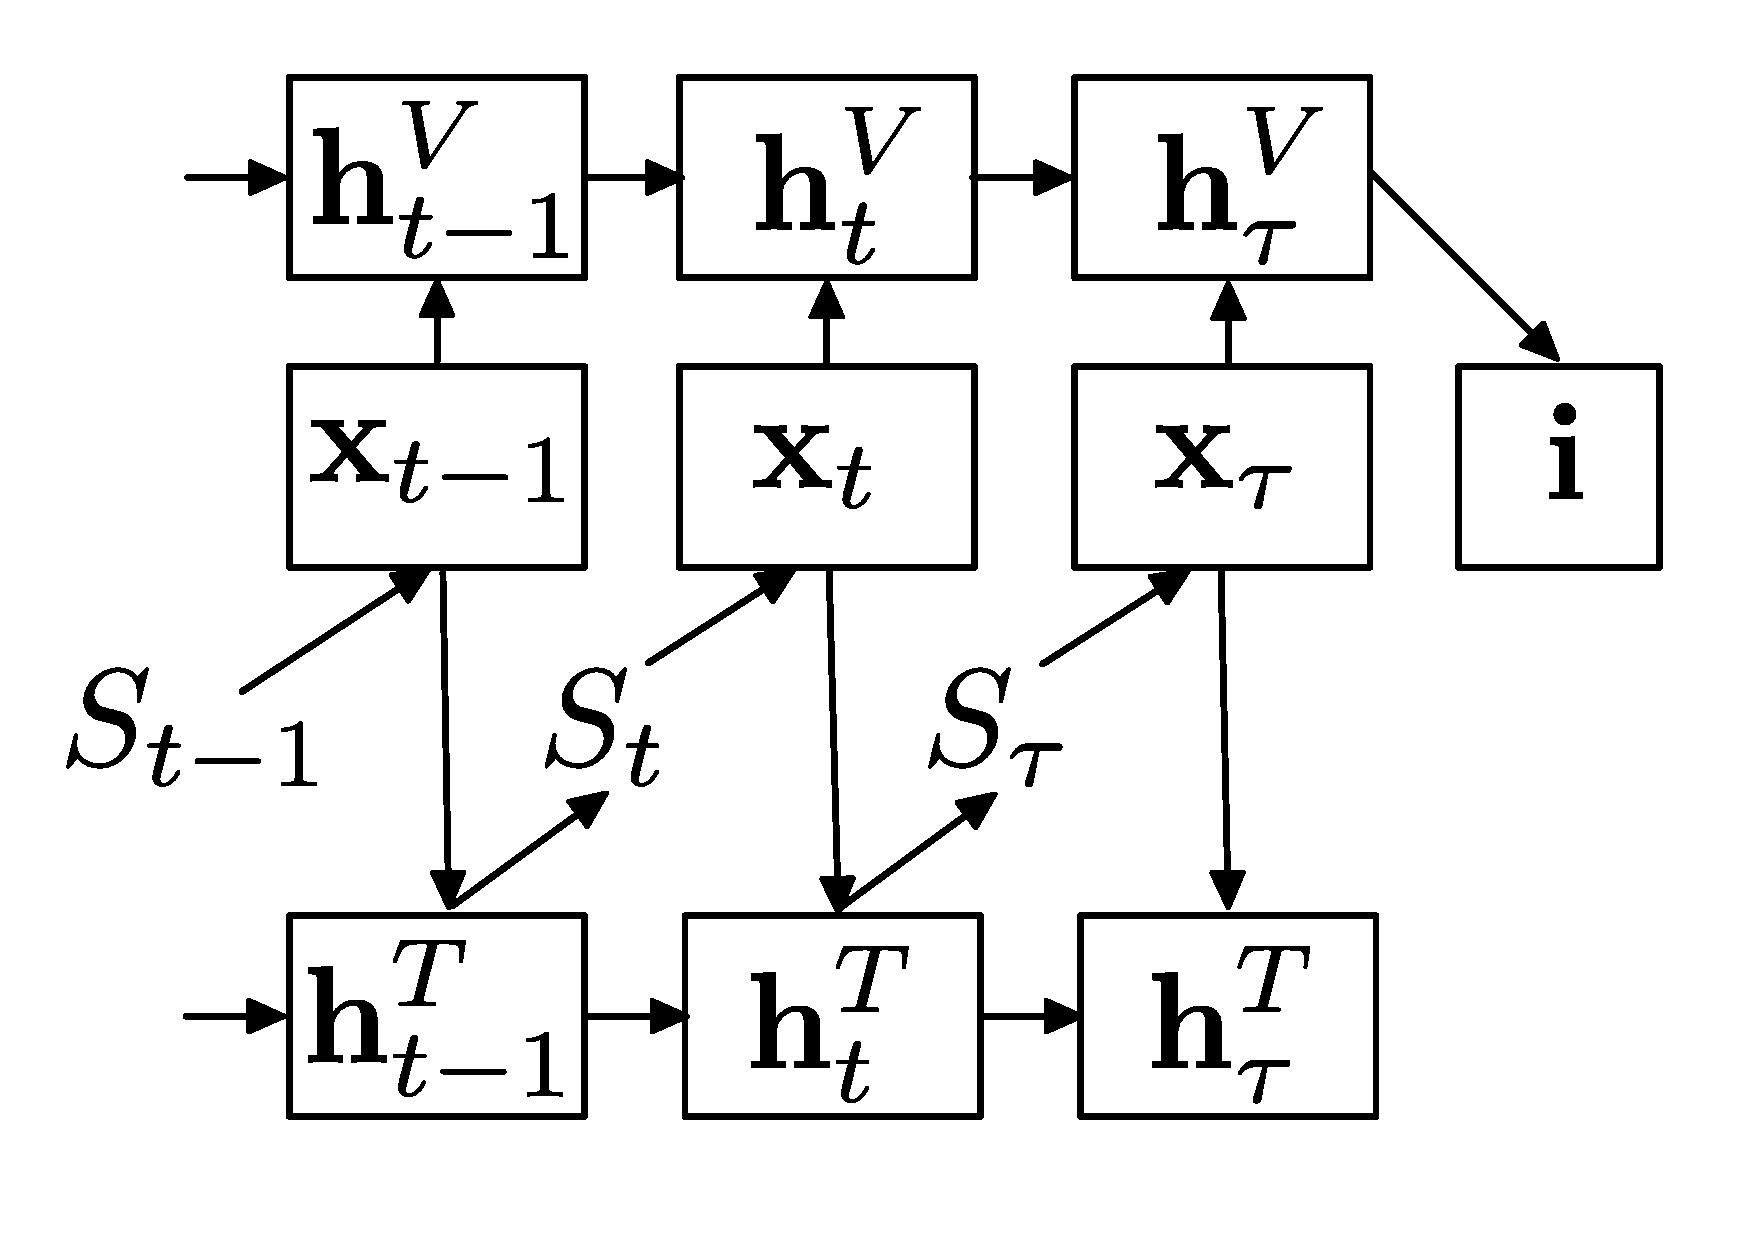
\includegraphics[scale=0.2]{imaginet.pdf} 
\caption{Structure of {\sc Imaginet}, adapted from \protect\cite{chrupala2015learning}.}
\label{fig:imaginet}
\end{center}
\end{figure}

Figure~\ref{fig:imaginet} shows the structure of {\sc Imaginet}. As can
be seen from the figure, the model consists of two GRU pathways, 
{\sc Textual} and {\sc Visual}, with a shared word-embedding matrix. 
The inputs to the model are pairs of image descriptions and their 
corresponding images. The {\sc Textual} pathway predicts the next 
word at each position in the sequence of words in each caption, whereas the 
{\sc Visual} pathway predicts a visual representation of the image that depicts the 
scene described by the caption after the final word is received.

Formally, each sentence is mapped to two sequences of hidden states, 
one by {\sc Visual} and the other by {\sc Textual}:
\vspace{-.2cm}
\begin{align}
  \mathbf{h}^{V}_t = \mathrm{GRU}^V(\mathbf{h}^{V}_{t-1},\mathbf{x}_t)\\
  \mathbf{h}^{T}_t = \mathrm{GRU}^T(\mathbf{h}^{T}_{t-1},\mathbf{x}_t)
\vspace{-.1cm}
\end{align}
%
At each time step {\sc Textual} predicts the next word in the sentence
$S$ from its current hidden state $\mathbf{h}^{T}_t$, while {\sc
  Visual} predicts the image-vector\footnote{Representing the full image, 
  extracted from the pre-trained Convolutional Neural Network of 
  \namecite{simonyan2014very}. \label{edit:dumdumeddy}}
$\hat{\mathbf{i}}$ from its last
hidden representation $\mathbf{h}^{V}_t$.
%
\vspace{-.2cm}
\begin{align}
   \hat{\mathbf{i}} &= \mathbf{V} \mathbf{h}^{V}_\tau \\
    p(S_{t+1}|S_{1:t}) &= \mathrm{softmax}(\mathbf{L}\mathbf{h}^T_t)
\vspace{-.1cm}
\end{align}
%
The loss function is a multi-task objective which penalizes error on
the visual and the textual targets simultaneously. The objective
combines cross-entropy loss $L^{T}$ for the word predictions
and cosine distance $L^V$ for the image
predictions\footnote{Note that the original formulation in
  \namecite{chrupala2015learning} uses mean squared error instead; as the performance of
{\sc Visual} is measured on image-retrieval which is based on cosine 
distances, we use cosine distance as the visual loss here.}, weighting them with the parameter $\alpha$ (set to $0.1$).
%
%\vspace{-.2cm}
\begin{align}
%\begin{equation}
%\label{eq:lossce}
&L^{T}(\theta) = {-} \frac{1}{\tau}\sum_{t=1}^\tau \log p(S_t|S_{1:t}) \\
%\end{equation}
%
%\vspace{-.2cm}
%\begin{equation}
%\label{eq:losscos}
&L^V(\theta) =  1 - \frac{\hat{\mathbf{i}} \cdot \mathbf{i}}{\| \hat{\mathbf{i}} \| \| \mathbf{i} \|} \\
%\end{equation}
%
%\vspace{-.2cm}
%\begin{equation}
%\label{eq:losscombo}
&L = \alpha L^T + (1-\alpha)L^{V}
\end{align}
%L^V(\theta) &= \frac{1}{K}\sum_{k=1}^K(\hat{i}_k-i_k)^2
%

\noindent
For more details about the {\sc Imaginet} model and its performance
see \namecite{chrupala2015learning}. Note that we introduce a small change in
the image representation: we observe that using standardized image
vectors, where each dimension is transformed by subtracting the mean
and dividing by standard deviation, improves performance.


%\todo{should we include somewhere where the image representations are coming from?}
% The model achieves near state-of-the-art results on MS-COCO image
% retrieval and good performance on other natural language
% understanding tasks. For the detailed results and more information
% please consult

% he model performance was evaluated on the test on image-retrieval
% and paraphrase retrieval - we consider captions belonging to the
% same image as paraphrases. Image retrieval is performed by the {\sc
% Visual} pathway by projecting the validation captions to the image
% space and ranking the images according to there cosine similarity to
% the projection. The model achieves a performance of Recall@1=0.06,
% Recall@5=0.20 and Recall@10=0.29. The paraphrase retrieval task is
% performed using the last hidden states of {\sc Textual} or {\sc
% Visual} to represent the captions in the validation set. As
% demonstrated by Table \ref{tab:retrieval} the representations
% computed by {\sc Textual} captures the paraphrase relationship
% better in the particular setting.



\subsection{Unimodal language model}
The model {\sc LM} is a language model analogous to the {\sc Textual}
pathway of {\sc Imaginet} with the difference that its word embeddings
are not shared, and its loss function is the cross-entropy on word
prediction. Using this model we remove the visual objective as a
factor, as the model does not use the images corresponding to captions
in any way.

\subsection{Sum of word embeddings}
The model {\sc Sum} is a stripped-down version of the {\sc Visual}
pathway, which does not share word embeddings, only uses the cosine
loss function, and replaces the GRU network with a summation over word
embeddings. This removes the effect of word order from
consideration. We use this model as a baseline in the sections which
focus on language structure. 

\section{Experiments}
\label{sec:experiments}


In the following section, we report a series of experiments in which
we explore the kinds of linguistic regularities the networks learn from
word-level input. Sections~\ref{sec:computeomission} to \ref{sec:beyondlexical} 
present the analyses of the final hidden activation 
vectors of the recurrent pathways from a linguistic point of view. 
Sections~\ref{sec:syntacticdim} and \ref{seq:describe} report exploratory experiments on
the linguistic features encoded by individual hidden dimensions. 
In all these experiments we report our findings based on the {\sc Imaginet}
model, whenever appropriate compare to our two other models {\sc LM} and {\sc Sum}, 
and discuss the generalizabilty of our methods to other architectures.
\label{edit:experimentsgeneral}
For all the experiments, we trained the models on the training portion of the
MSCOCO image-caption dataset \cite{lin2014microsoft}, and analyzed the
representations of the sentences in the validation set corresponding
to 5000 randomly chosen images. The target image representations were
extracted from the pre-softmax layer of the 16-layer CNN of
\namecite{simonyan2014very}.

% \iffalse

% {\bf Section~\ref{sec:macro}} includes experiments that provide linguistic analysis of the activation patterns on the activation vector level with results more quantitative in nature. Section~\ref{sec:salience} describes a method to estimate the salience of tokens as a function of their part-of-speech category and grammatical function (dependency relation) in sentences. 

%  Sections~\ref{sec:gramfunc} and \ref{subsec:information-struct} apply this method and provide evidence that the {\sc Visual} pathway of {\sc Imaginet} learns to interpret the same word fullfilling different grammatical functions differently, and is sensitive to the information structure of sentences.


% {\bf Section~\ref{sec:micro}} compliments the macro level analysis and reports a series of more qualitative experiments exploring the kinds of linguistic abstraction represented by individual hidden units. Section~\ref{sec:reprdim} proposes a simple method for representing
% the function of hidden units by identifying the top K contexts that yield the highest activation values, and Section~\ref{sec:topk} provides a general qualitative analysis of these contexts.

% For the experiments using the {\sc Imaginet} model we use the validation set of MS-COCO.
% Finally Section~\ref{sec:syntacticdim} goes more into detail and shows examples 
% of hidden units that are active for particular multi-word constructions with joint
% semantical and syntactic regularities.  
% \fi





%\begin{enumerate}
%\item How accurately does each model represent syntactic knowledge? WE DONT DO THIS
%\item What types of grammatical functions each model pays most attention to? WE DO THIS
%\item What is the level of separation between syntactic and semantic 
%representations learned by the models? NO CHANCE
%\item What functions are the individual units in each network specialized for? WE DO THIS 
%\item On each of the above dimensions, what are the systematic differences 
%between models that are optimized for different tasks?  WE ALSO DO THIS
%\end{enumerate}



%Section~\ref{sec:categories} looks at the salience of two sets of syntactic categories in 
%each model, by estimating how much input tokens from each category influence 
%the final performance in each task. In Section~\ref{sec:syntax}, we examine the 
%degree to which syntactic information is encoded in the internal representations 
%acquired by each model. Section~\ref{sec:dimension} focuses on analyzing the 
%reaction patterns of individual units in each model, and on finding out specialized 
%functions that these units perform. 

%Finally in Section~\ref{sec:visualize}, we look at 
%how the meaning representations of word sequences evolve over time for each 
%model. \todo{not sure how to relate this last one to our objectives.}
%In all our experiments, we compare the nature and degree of the acquired 
%syntactic knowledge among models that are trained for performing different tasks.


%\noindent{\bf Syntactic categories.} In all the following analyses, we use two different sets of syntactic categories: part-of-speech categories (POS) and dependency relations (DepRel). The tagging is performed jointly using the TurboParser dependency parser\footnote{This implementation is available at https://github.com/andre-martins/TurboParser.} \cite{martins2013turning}. For POS tags we use the Penn Treebank tagset and for the dependency relations the Stanford basic dependencies.



%\section{Representing syntactic information}
\label{sec:regression}

It is assumed that to perform a task that involves some level of language 
understanding, RNNs need to learn some level syntactic knowledge from the 
linguistic input. To uncover if the networks indeed represent syntactic 
information, we trained a number of Logistic Regression models on various 
combinations of n-gram tokens in the input as well as the hidden states of the 
networks to predict the syntactic categories of the tokens at each time-step $t$. 
From the sentences we extracted unigram and n-gram features up to a window 
size of 4; for example, to predict the label for {\it dog} in the sentence {\it the nice 
dog} we extract {\it the}$_2$, {\it nice}$_1$, {\it dog}$_0$, {\it the$_2$ nice$_1$}, 
{\it nice$_1$ dog$_0$}, and {\it the$_2$ nice$_1$ dog$_0$}, etc. 

We trained several models on a combination of the following features:
\begin{itemize}
  \item current word $w_t$
  \item current word-embedding of {\sc Imaginet} $e_t^I$ (same for {\sc Visual} 
and {\sc Textual})
  \item current word-embedding of {\sc Sentiment} $e_t^S$
  \item 4-gram features
  \item hidden state of {\sc Visual} $h_t^V$
  \item hidden state of {\sc Textual} $h_t^T$
  \item hidden state of {\sc Sentiment} $h_t^S$
%  \item hidden state of {\sc Visual} $h_t^V$ + 4-gram features
%  \item hidden state of {\sc Textual} $h_t^T$ + 4-gram features
\end{itemize}

The motivation behind this experiment is that if the networks generalize over 
syntactic categories, then using their activation vectors as features will lead to a 
more accurate model f$h_t$or syntactic category prediction than only using the tokens 
themselves. If the embeddings $e_t$ and hidden activations $h_t$ outperform 
the word form $w_t$ and 4-gram models respectively, then the linguistic 
representations of the model do generalize over syntactic categories.


\begin{table}[]
\centering
\caption{Results of predicting syntactic categories for each token in the input to 
SENTIMENT and IMAGINET models, by Logistic Regression classifiers trained 
on features in the first column. The second and third columns report the micro F-
scores on DepRel and POS categories respectively.}

\label{tab:logistic}
\begin{tabular}{lll}
\hline
 \multicolumn{3}{c}{\sc Sentiment}           \\
 \hline 
{\bf Features}      &  {\bf deprel} &  {\bf POS}     \\
\hline 
word $w_t$                   		  & .50  & .65   \\
4-gram                       		  & .62  & .71   \\
$e^S_{t}$          & .33  & .38   \\ 
$h_t^S$                      		  & .30  & .32    \\
\hline 
\hline
\multicolumn{3}{c}{\sc Imaginet}                          \\
 \hline 
{\bf Features}      &  {\bf deprel} &  {\bf POS}     \\
\hline 
$w_t$                   		  	      & .710   & .93  \\
4-gram                         		  & .807  & .93  \\
$e^I_{t}$          			  	      & .73   & .95  \\ 
$h_t^V$                      		  & .751  & .88  \\
$h_t^T$                      		  & .811  & .94  \\
$h_t^T$ + $h_t^V$            		  & .81   & .94  \\
$h_t^V$ + 4-gram             		  & .809   & .93  \\
$h_t^T$ + 4-gram             		  & .823   & .95
\end{tabular}
\end{table}

Table~\ref{tab:logistic} shows the results of predicting the syntactic categories of 
tokens in the input sentences using different (combinations of) features. 
\todo{Are we going to change this to test set?}

The results for {\sc Sentiment} show that the representations (both 
$e^S_{t}$ and $h_t^S$) are less predictive of the grammatical categories of the 
target words than using the unigram and 4-gram features.

%In fact there are only 8 categories out of 44 with non-zero f-scores for deprels: 
%amod (0.28), cc (.64), conj (.13), det (.56), nsubj (.29), pobj (.30), prep (.43) and 
%root (.26).
However, in case of {\sc Imaginet}, using the embeddings $e_t$ leads to higher F-score for both dependency category and part-of-speech tag prediction of the tokens $w_t$ than using $w_{t}$'s 
themselves. This result provides evidence that syntactic information is indeed encoded in the learned word embeddings. 
Similarly, the classifier trained on the hidden activations of {\sc Textual } $h_t^T$ 
performs better on both DepRel and POS prediction than using 4-grams features, but only by a 
narrow margin. 

The more interesting results, however, are the low F-scores when 
using $h_{t}^V$ as features. These results suggest that {\sc Visual} represents less 
syntactic information then {\sc Textual} about sequences of words. We also observe 
that the maximum F-score is achieved using the combinations of $h_{t}^T$ and the 4-
gram features, suggesting that perhaps some information about the word identities is 
lost in $h_{t}^T$.

%\section{Analysis of hidden activation vectors}
%\label{sec:macro}

% \begin{figure*}[t]
% \hspace*{-0.5in}
% \setlength{\tabcolsep}{0.01pt}
%     \begin{tabular}{cccc}
%     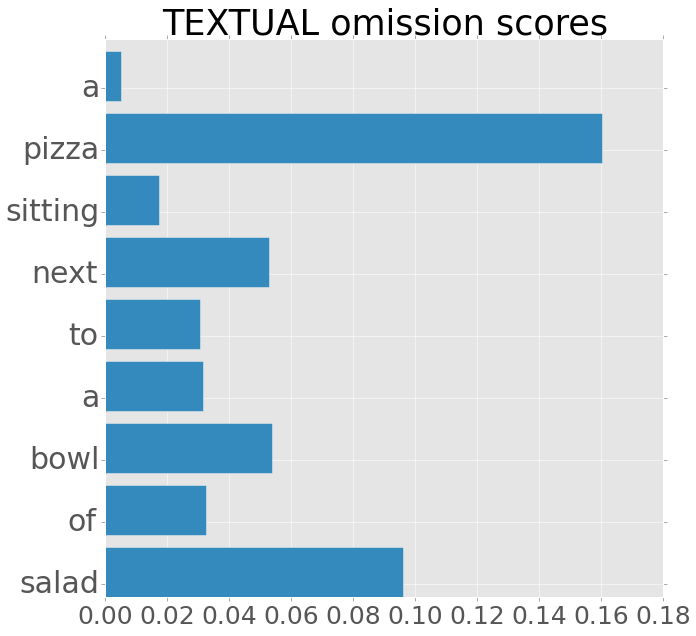
\includegraphics[scale=0.14]{new_omission_examples/textual1} &
%     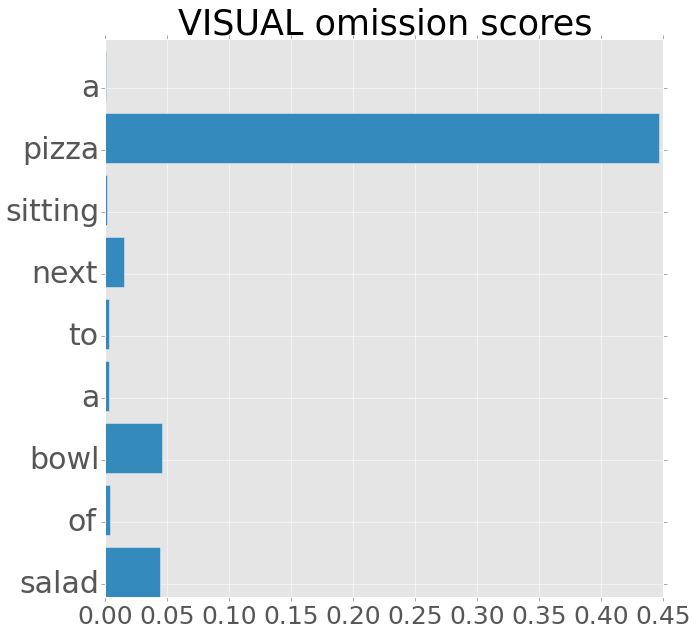
\includegraphics[scale=0.14]{new_omission_examples/visual1} &
%     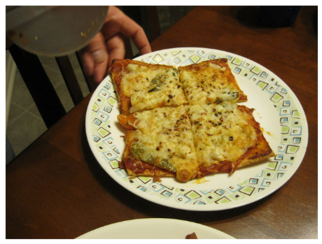
\includegraphics[scale=0.33]{new_omission_examples/img1} & 
%     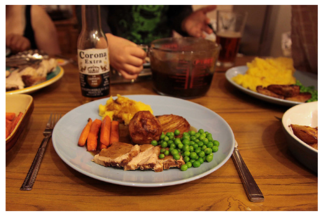
\includegraphics[scale=0.28]{new_omission_examples/img1_omit} \\
%     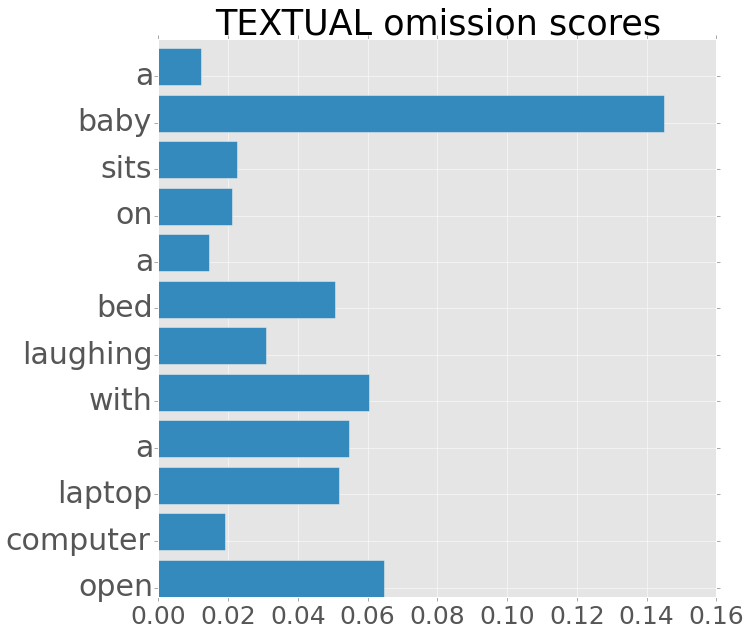
\includegraphics[scale=0.16]{new_omission_examples/textual2} &
%     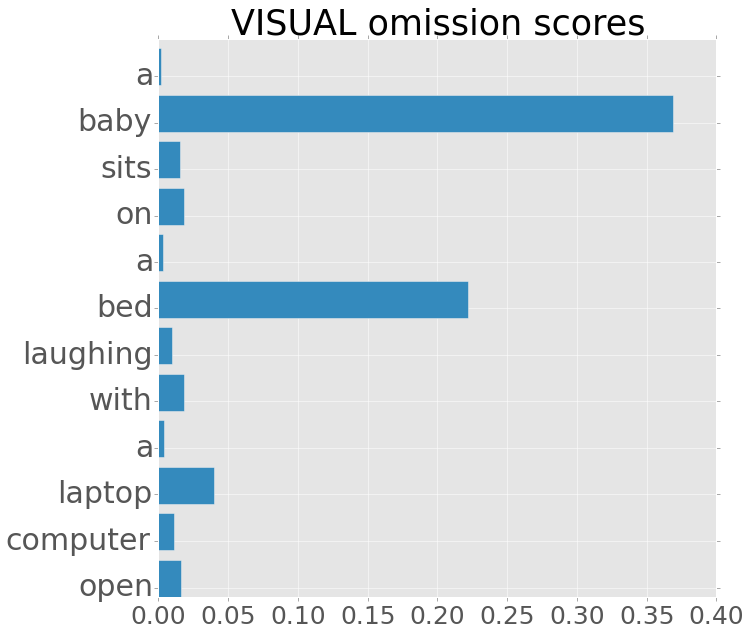
\includegraphics[scale=0.16]{new_omission_examples/visual2} &
%     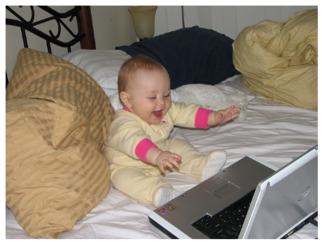
\includegraphics[scale=0.28]{new_omission_examples/img2} & 
%     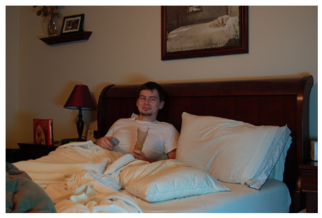
\includegraphics[scale=0.30]{new_omission_examples/img2_omit}
%     \end{tabular}
%     \caption{The omission scores of {\sc Visual} and {\sc Textual} for two example sentences, 
% and the best retrieved images for the original sentence (left) and the sentence with the most 
% important word removed (right). 
% %Top row example caption is {\it a bottle next to a windowsill with
% %  light coming through},  bottom row: {\it a train on a track next to
% %  many bushes}.
% }
%     \label{fig:omissionex}
% \end{figure*}


\begin{figure*}[t]
  \centering
  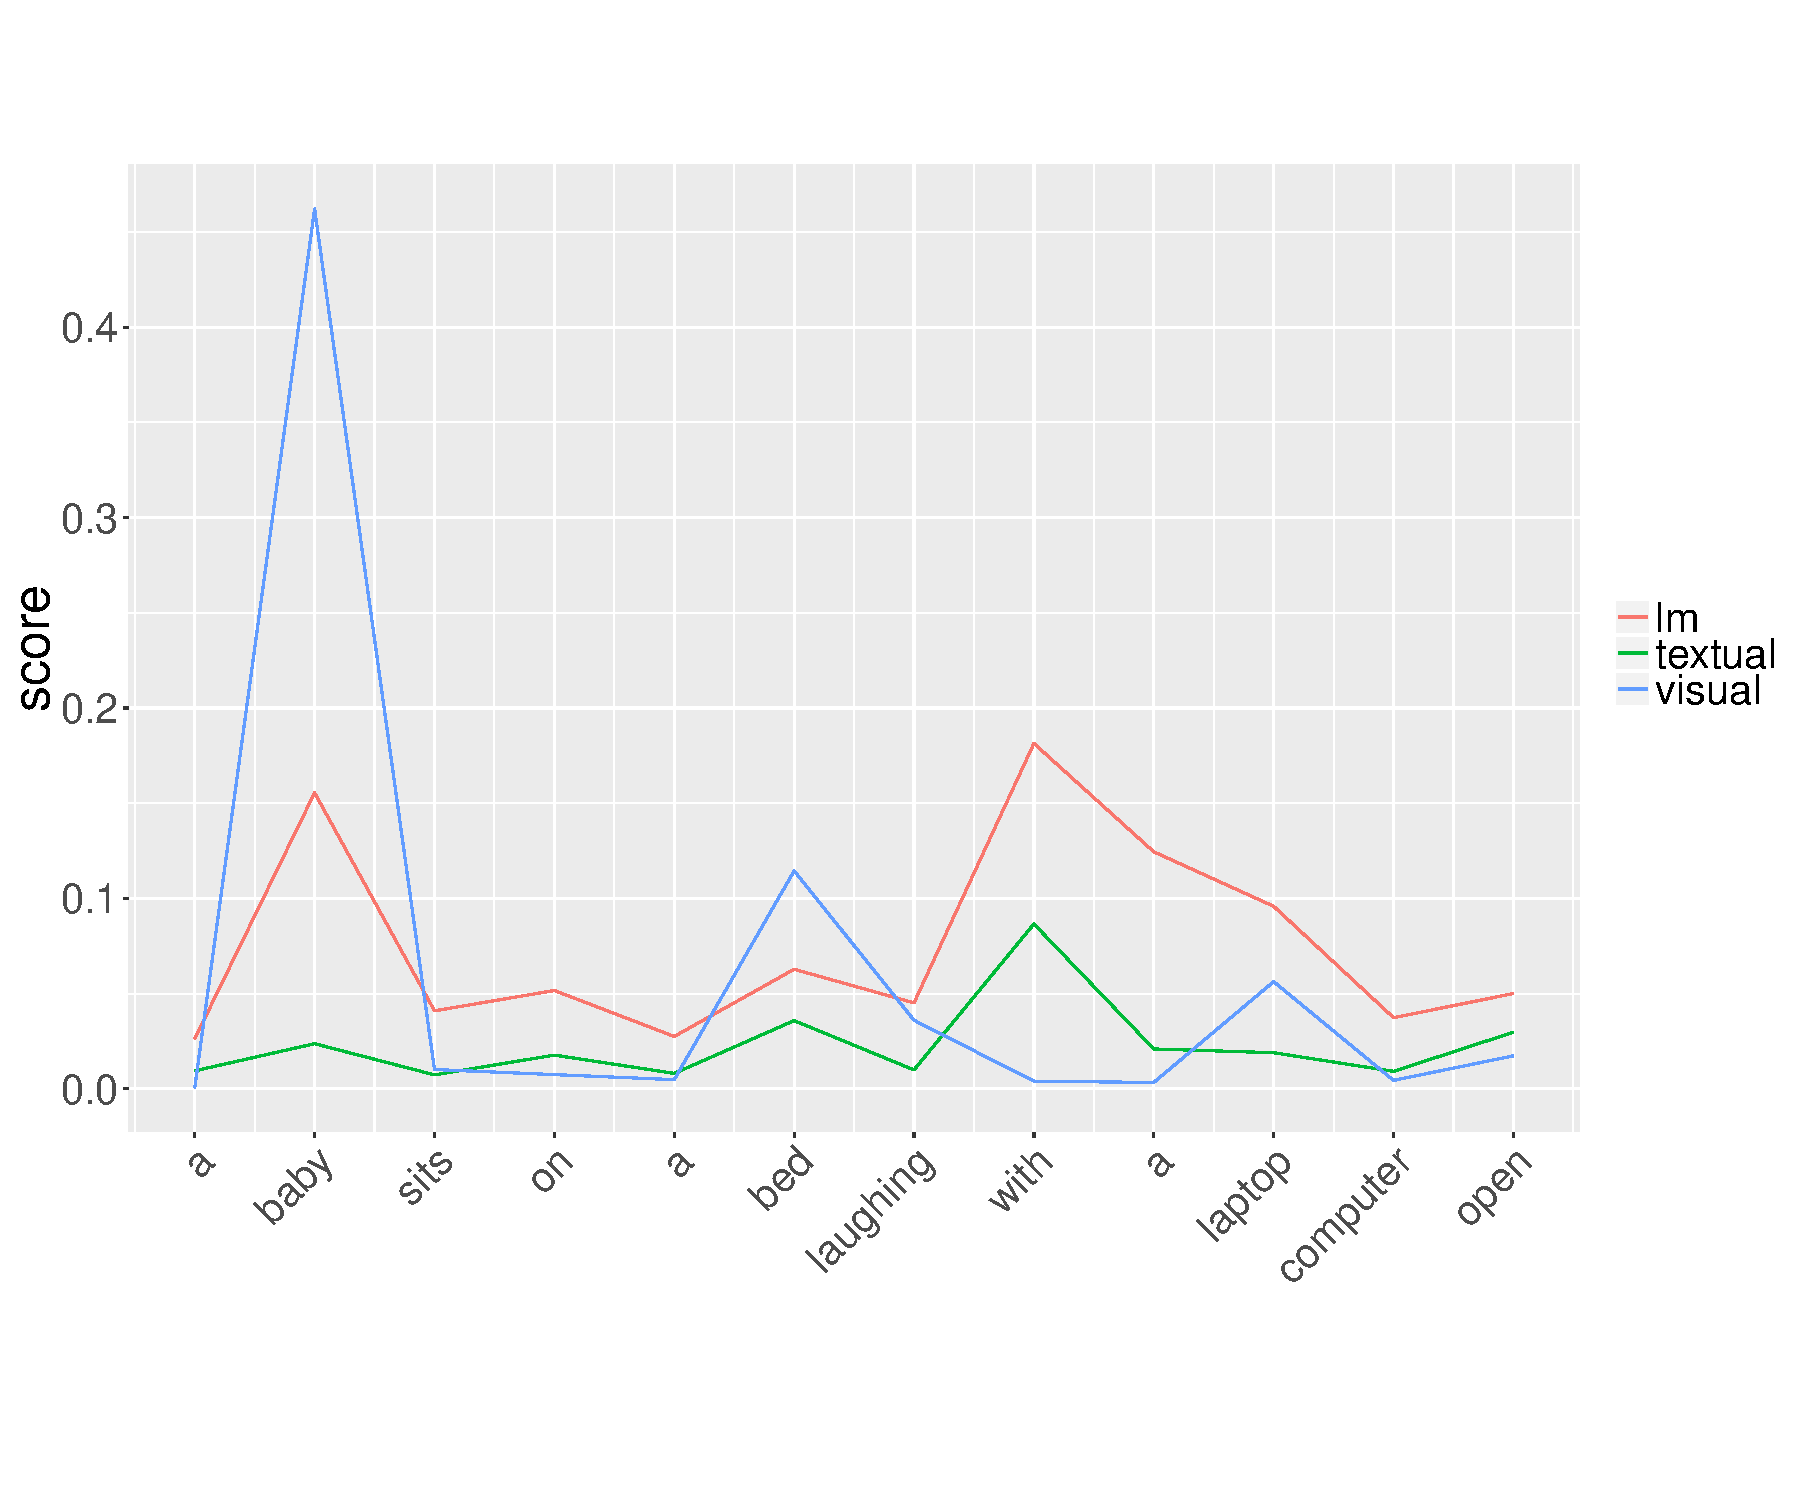
\includegraphics[scale=0.3]{omissionex.pdf}
  \caption{Omission scores for the example sentence {\it a baby sits
      on a bed laughing with a laptop computer open} for {\sc LM} and
    the two pathways, {\sc Textual} and {\sc Visual}, of {\sc
      Imaginet.}}
  \label{fig:omissionex}
\end{figure*}

\begin{figure*}[t]
  \centering
  
\includegraphics[scale=0.25]{85826.jpg}
  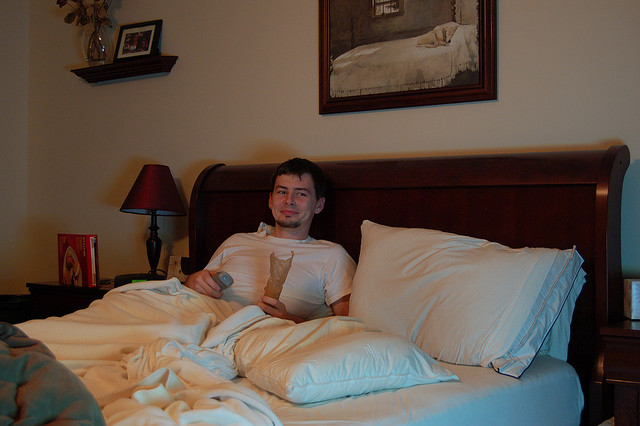
\includegraphics[scale=0.25]{60596.jpg}
  \caption{Images retrieved for the example sentence {\it a baby sits
      on a bed laughing with a laptop computer open} (left) and the
    same sentence with the second word omitted (right).}
  \label{fig:omissionexpic}
\end{figure*}





%Understanding the behavior of the learned models in terms of which features do they assign 
%the most attention to is straight forward with linear 
%models such as linear/logistic regression, 
%naive-bayes classifiers or with some of the non-parametric models as well such as decision 
%trees. This information allows researchers to not only train learning algorithms to perform 
%particular tasks, but also to uncover some underlying patterns in the training data. 
 
%\subsection{Salience of categories of words}
%\label{sec:salience}
%In this section we propose novel techniques for interpreting the
%activation patterns of neural networks trained on language tasks
%from a linguistic point of view and focus
%on the high level understanding of what parts of input sentence the networks
%pay most attention to. Furthermore, we investigate if the networks
%learn to assign differential amounts of importance to tokens depending
%on their position and grammatical function in the sentences.\label{edit:whyposdep}
%In Section~\ref{sec:computeomission} we introduce \emph{omission scores};
%a metric to measure the contribution of each token to the prediction
%of the networks and in Section~\ref{sec:omitimaginet} we analyze how
%these scores are distributed over dependency relations and
%part-of-speech categories. 
%In Section~\ref{sec:beyondlexical} we investigate the extent to which
%the importance of words for the different networks depend on the words themselves,
%their sequential position and their grammatical function in the sentences.
% MAYBE THIS WOULD BE TOO MUCH
%We apply the proposed methods to explore
%the representations of {\sc Imaginet}, but also discuss how to generalize
%them to other architectures.

\subsection{Computing Omission Scores}
\label{sec:computeomission}

We propose a novel technique for interpreting the
activation patterns of neural networks trained on language tasks
from a linguistic point of view, and focus
on the high-level understanding of what parts of input sentence the networks
pay most attention to. Furthermore, we investigate if the networks
learn to assign different amounts of importance to tokens depending
on their position and grammatical function in the sentences.\label{edit:whyposdep}

In all the models the full sentences are represented by the
activation vector at the end-of-sentence symbol
($\mathbf{h}_\text{end}$). We measure the salience of each word $S_i$
in an input sentence $S_{1:n}$ based on how much the representation of the
partial sentence $S_{\setminus i} = S_{1:i-1}S_{i+1:n}$, with
the omitted word $S_i$, deviates from that of the original sentence
representation. For example, the distance
between $\mathbf{h}_\text{end}(${\it the black dog is running}$)$
and $\mathbf{h}_\text{end}(${\it the dog is running}$)$ determines
the importance of {\it black} in the first sentence. We introduce the
measure $\mathrm{omission}(i,S)$ for estimating the salience of a word $S_i$:

\begin{equation}
\label{eg:omit}
\mathrm{omission}(i,S) = 1-\mathrm{cosine}(\mathbf{h}_\text{end}(S),
\mathbf{h}_\text{end}(S_{\setminus i}))
\end{equation}

\noindent Figure~\ref{fig:omissionex} demonstrates the omission
scores for the {\sc LM}, {\sc Visual} and {\sc Textual} models for an
example caption. The omission scores are
plotted for the
full sentence and for the sentence with the word with the highest
$\mathrm{omission}(i,S)$ removed. 
Figure~\ref{fig:omissionexpic} shows the images retrieved by {\sc
  Visual} for the full
caption and for the one with the word {\it baby} omitted. 
The images are retrieved from the validation set of MS-COCO by: 1)
computing the image representation of the given sentence with {\sc
  Visual}; 2) extracting the CNN features for the images from the set;
and 3) finding the image that minimizes the cosine distance to the
query.\label{edit:retrievalexplain} 
The omission scores for {\sc Visual} show that the model paid attention
mostly to {\it baby} and {\it bed} and slightly to {\it laptop} and
retrieved an image depicting a baby sitting on a bed with a laptop.
Removing the word {\it baby} leads to an image that depicts an adult
male laying on a bed. Figure~\ref{fig:omissionex} also shows that in
contrast to {\sc Visual}, {\sc Textual} distributes
its attention more evenly across time steps instead of focusing on the
types of words related to the corresponding visual scene. The peaks
for {\sc LM} are the same as for {\sc Textual}, but the variance of
the omission scores is higher, suggesting that the unimodal language
model is more sensitive overall to input perturbations than {\sc Textual}.


%For other RNN architectures such as LSTMs \label{edit:omitgeneral}
%and their bi-directional variants, measuring the contribution
%of tokens to their predictions (or the omission scores)
%can be straight-forwardly computed using their hidden state 
%at the last time step used for prediction. Furthermore, the technique 
%can be applied in general to other architectures which
%map variable length linguistic expressions to the same fixed dimensional
%space and perform predictions based on these embeddings. 
%This includes tree-structured Recursive Neural Network models such as the Tree-LSTM
%introduced in \namecite{kai2015treelstm} or the CNN architecture of \namecite{yoonneural2014} 
%for sentence classification. In both cases the pre-softmax activations can be extracted 
%from the models as the representations of the full and partial sentences.   


% Given a corpus segmented into sentences, each word in an input sentence is tagged with its 
%part-of-speech category (POS) and dependency-relation (DepRel). For dependency relations 
%only the label of the ark (and not the ark itself) is taken into account. For each input sentence 
%of 
%length $n$ the RNNs produce $n$ hidden activation vectors $h_{1}, \ldots , h_{n}$. Each word 
%in the input sentence is tagged with POS and DepRel categories and the contribution of the $<
%$word, POS, DepRel$>$ tuples to the meaning of the sentence is measured by computing the 
%following scores:
% 

%\paragraph{$omission$} Given a sentence "the black dog", we generate 3 sentence by 
%omitting one of the words each time: "the black", "the dog", "black dog". For each of these 
%sentence we compute a sentence representation $h_{full}$ and calculate the cosine 
%similarities 
%between the original and the omitted sentences. This measured is used to indicate the overall 
%importance of word categories. \todo{Example with a short sentence: ab, bc, cd, cosines}
%\\

%-----------------
\subsection{Omission score distributions}
\label{sec:omitimaginet}

%\begin{figure*}
 %   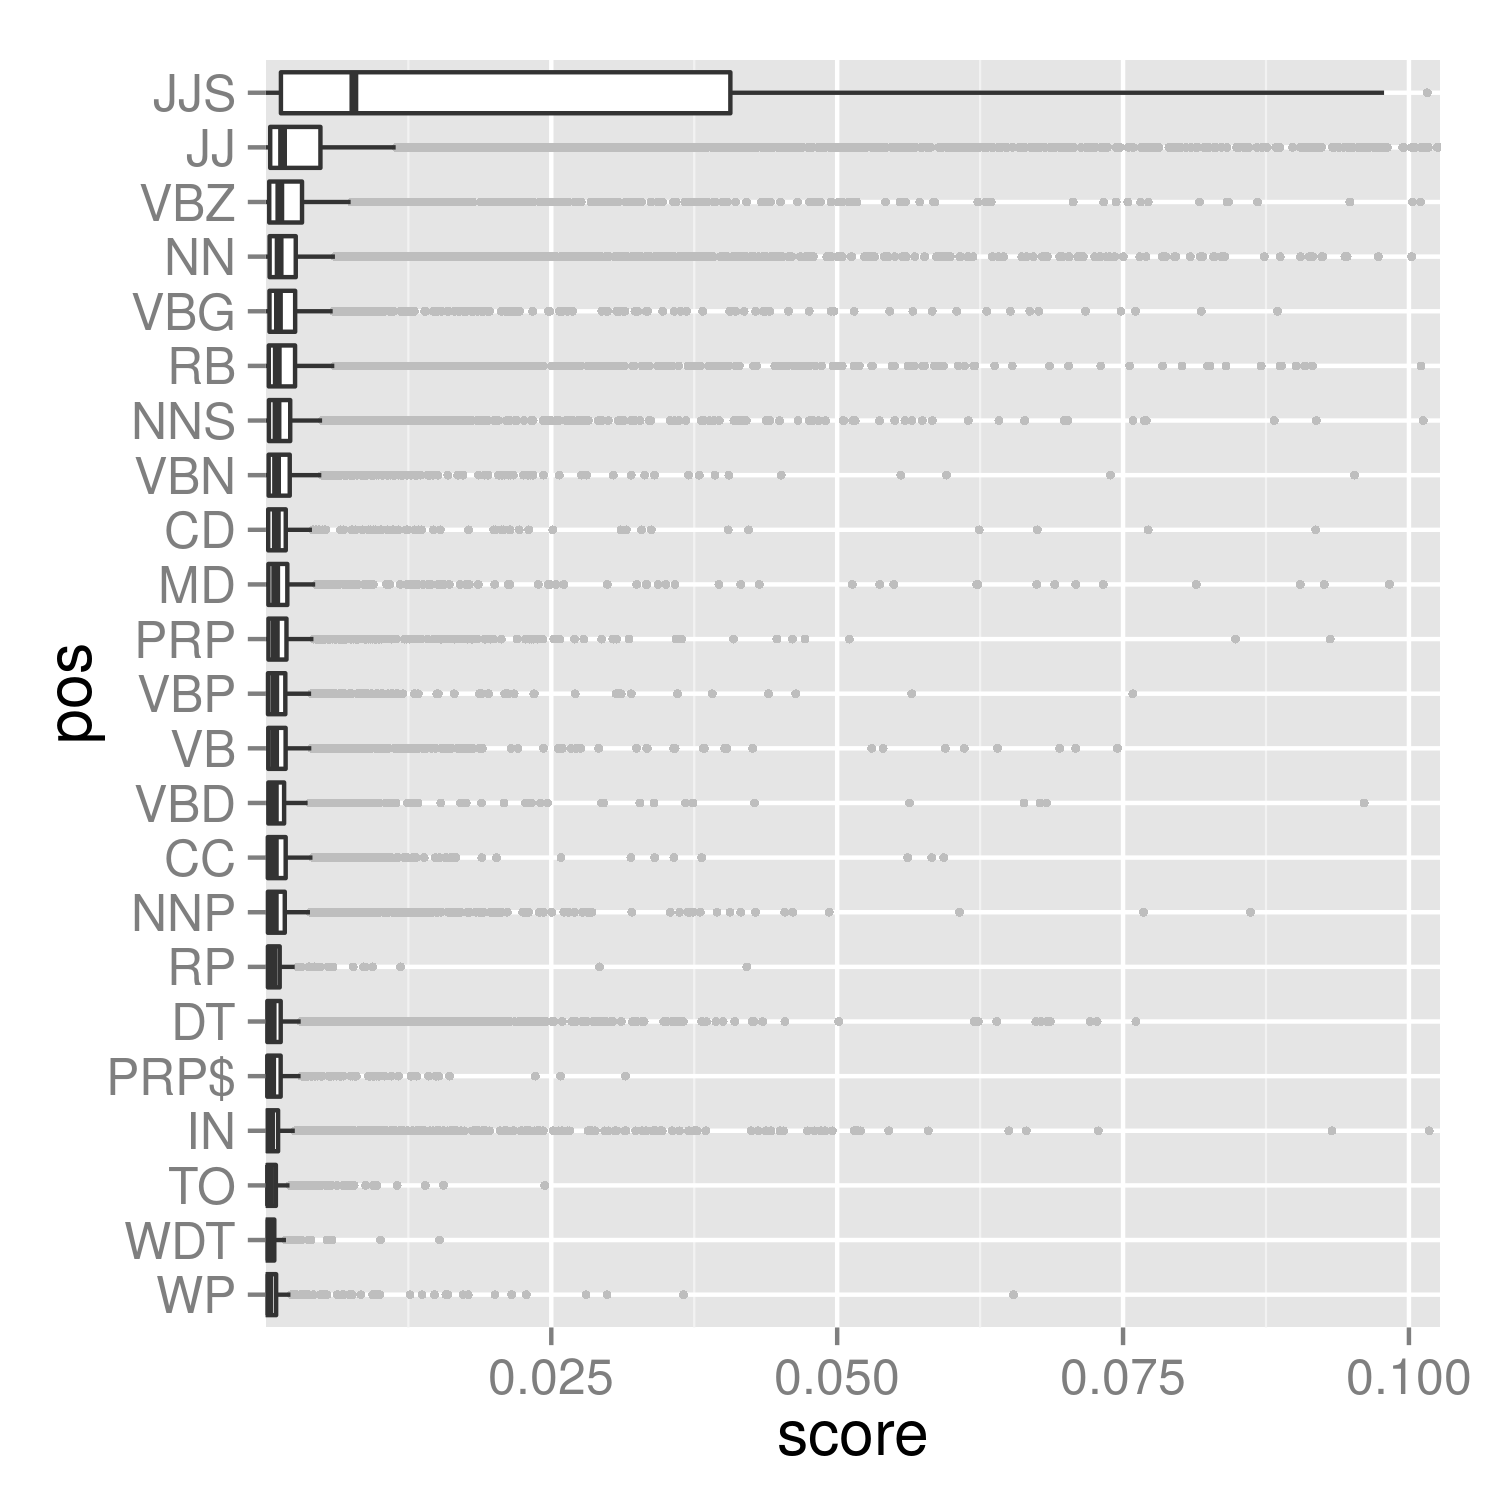
\includegraphics[scale=0.6]{omission-stat/sent-omission-pos-boxplot.png} 
 %   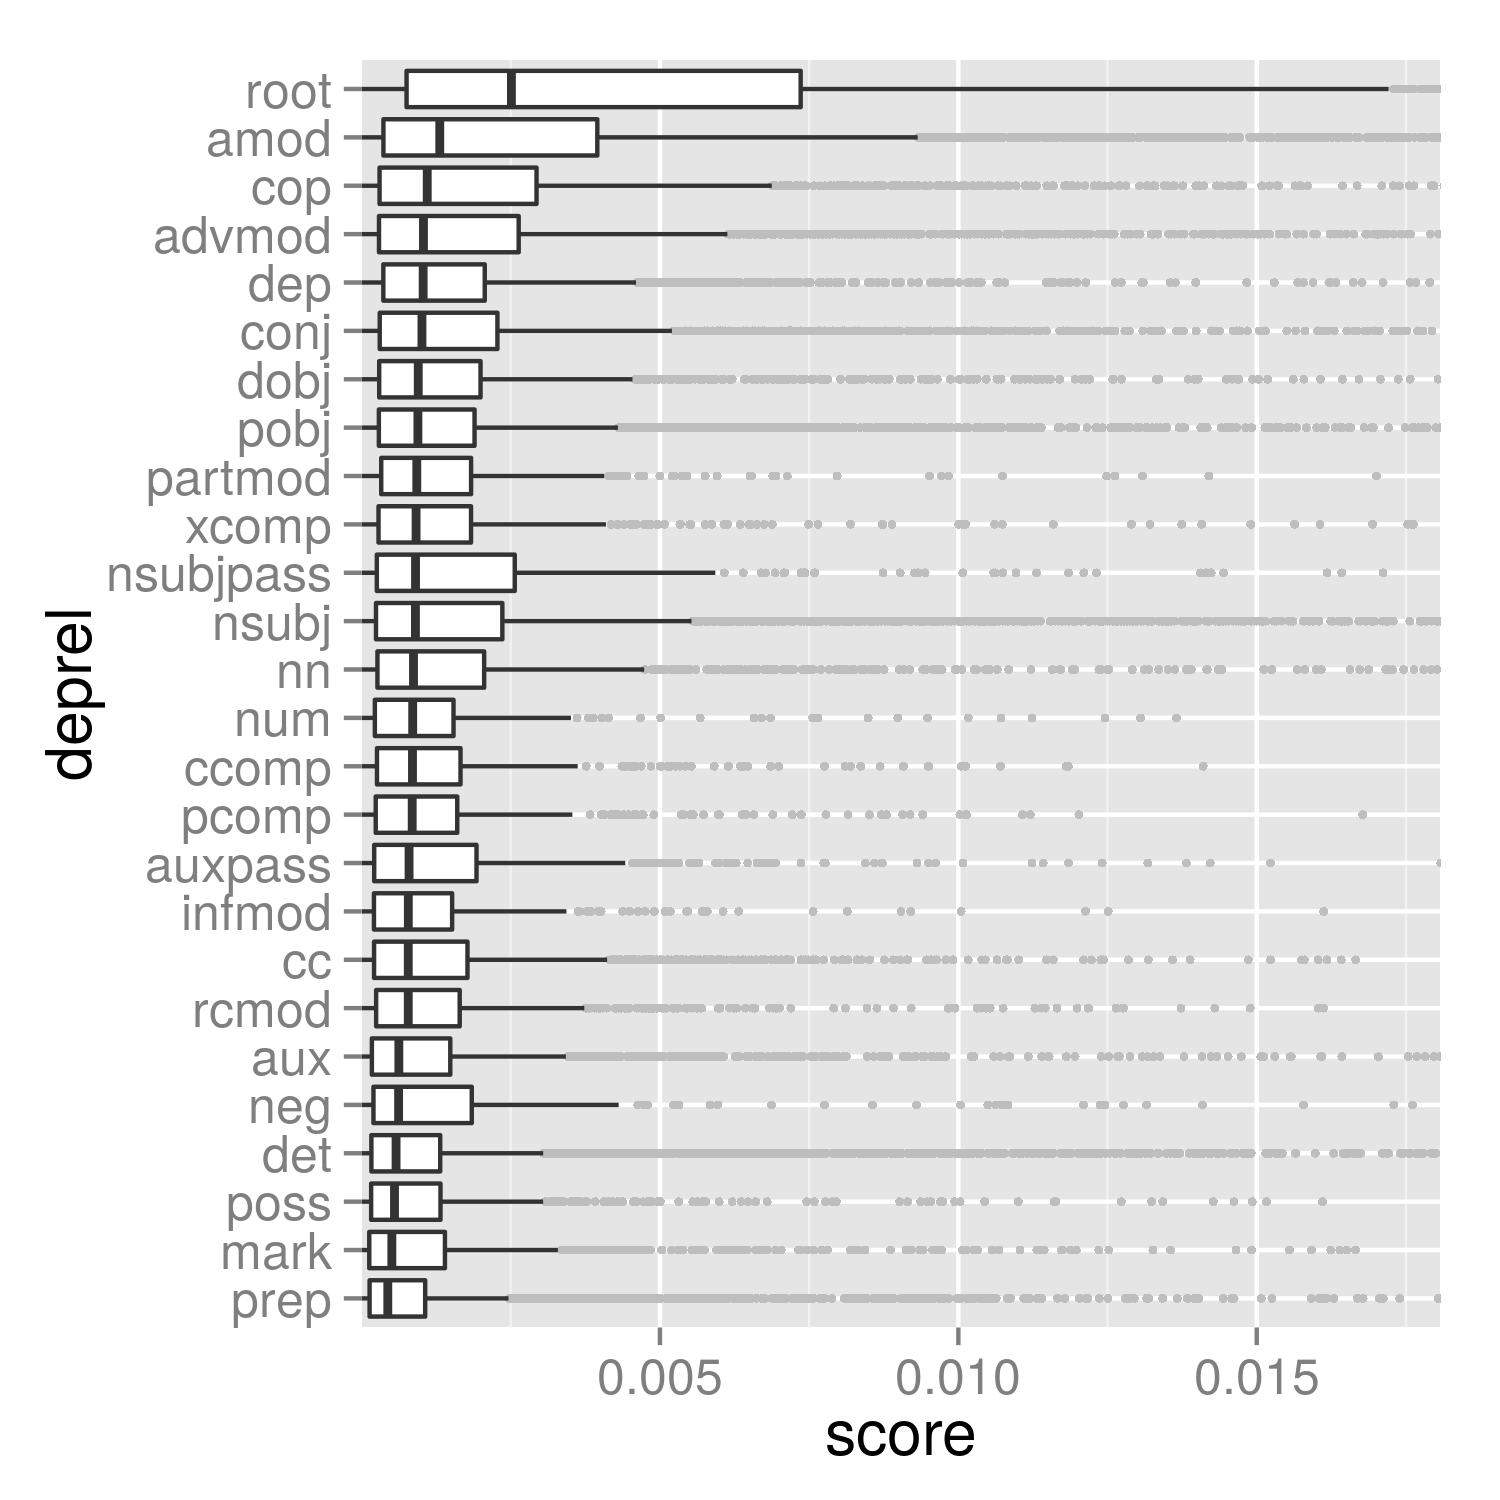
\includegraphics[scale=0.6]{omission-stat/sent-omission-deprel-boxplot.png} 
 %   \caption{Distributions of omission scores per POS category (left)
 %     and dependency relation (right) for {\sc Sentiment}. Only labels
 %   which occurred at least 300 times are included.}
%\label{fig:omission-sent}
%\end{figure*}

%\subsubsection{Omission results for {\sc Sentiment}}
%\label{sec:omitsentiment}
%Figure~\ref{fig:omission-sent} shows the distribution of the omission scores per category for the {\sc Sentiment} model. Superlative adjectives (JJS) such as {\it best, least, scaries} and {\it funniest} are by far the most influential POS category, followed by Adjectives (JJ), Verbs (VBZ, VBG), Nouns (NN, NNS) and Adverbs (RB). Similarly, tokens with function {\sc root} (various verbs, nouns or adjectives central to the meaning of the sentence) are recognized by the model as the most important category, followed by adjectival modifier {\sc amod}. These results support the validity of $\mathrm{omission}$ as a measure of saliency and provide evidence that {\sc Sentiment} learns representations that enable the model to successfully filter out irrelevant parts of the input. 

%-----------------
\label{subsec:omission-text-vis}
\begin{figure}[!htbp]
\centering
%\hspace*{-0.3in}
%\setlength{\tabcolsep}{0pt}
%  \begin{tabular}{cc}
  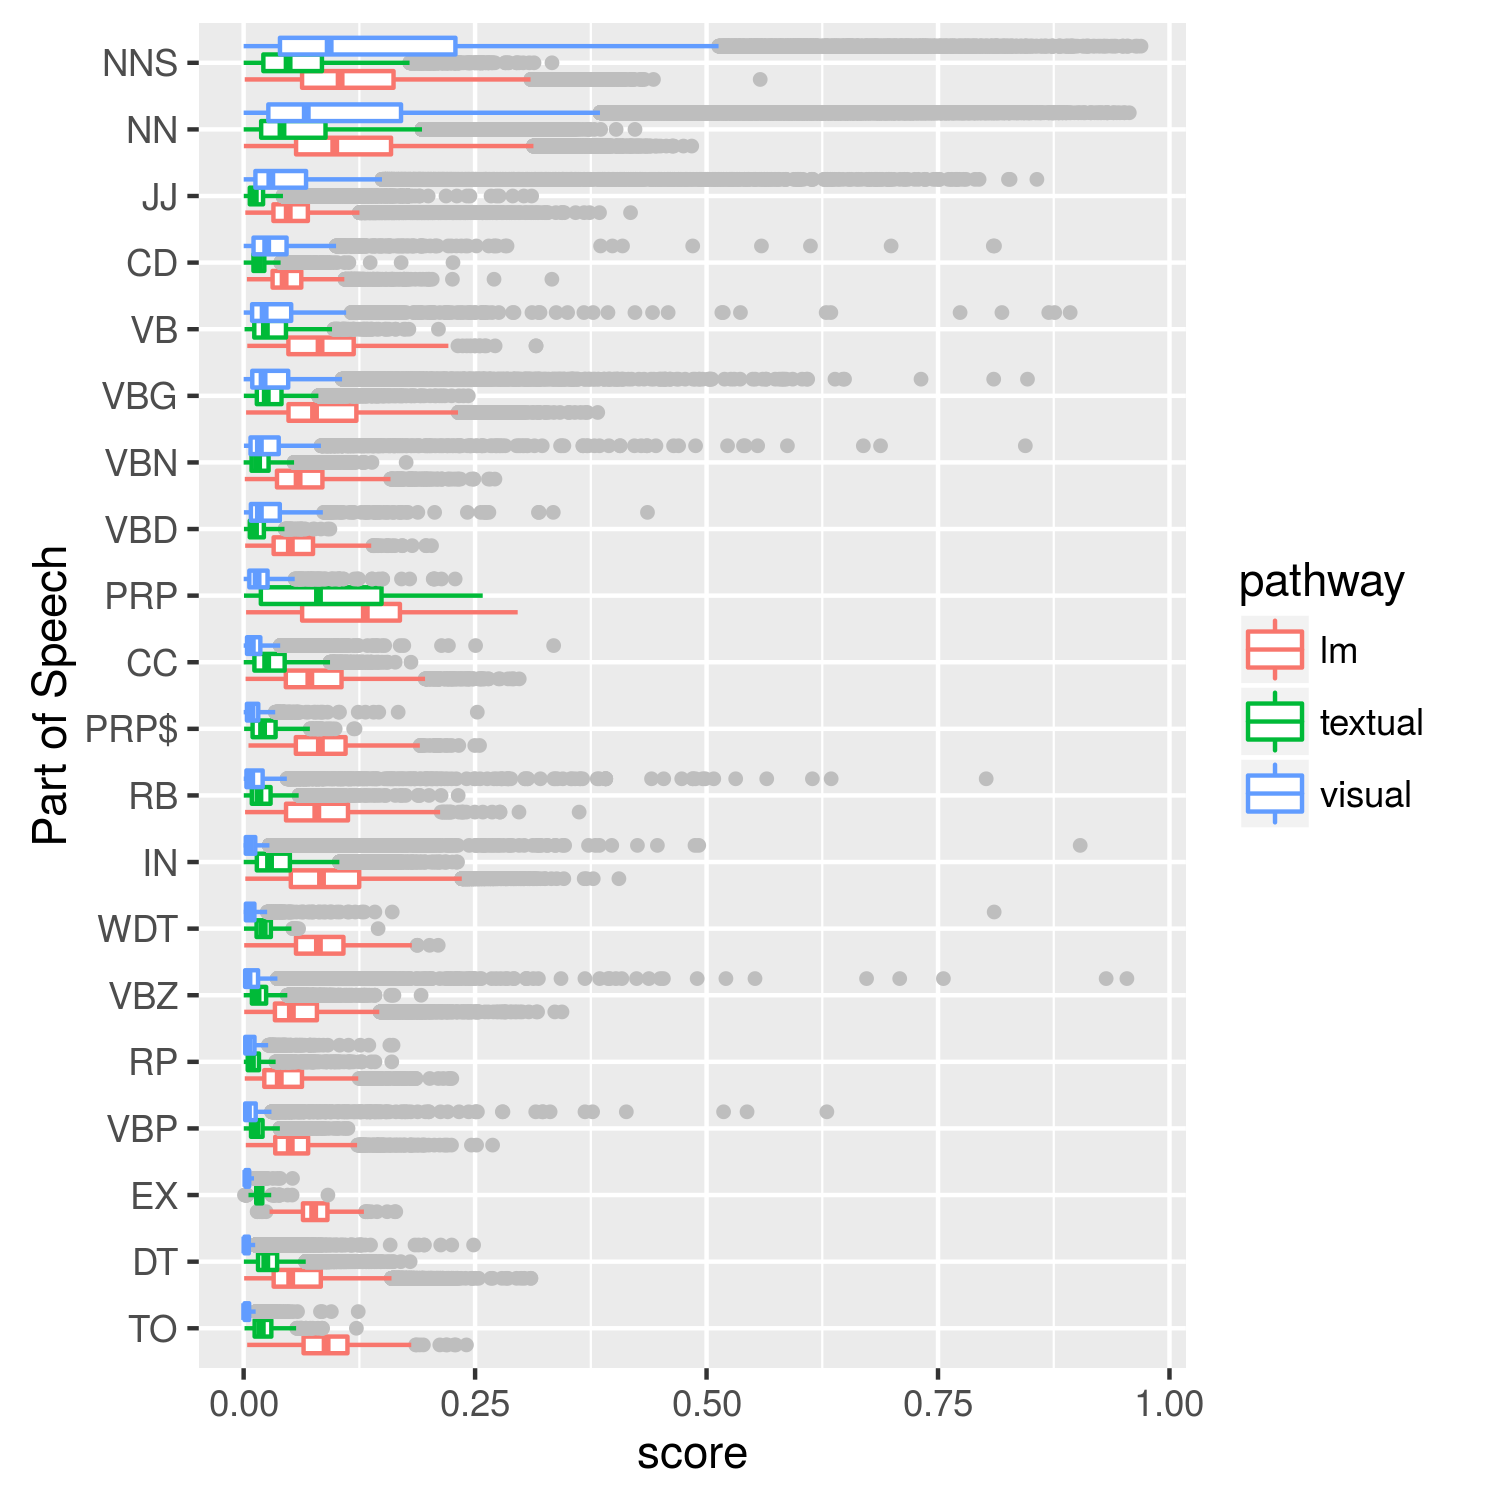
\includegraphics[scale=0.9]{imaginet-omission-pos-boxplot.png} 

  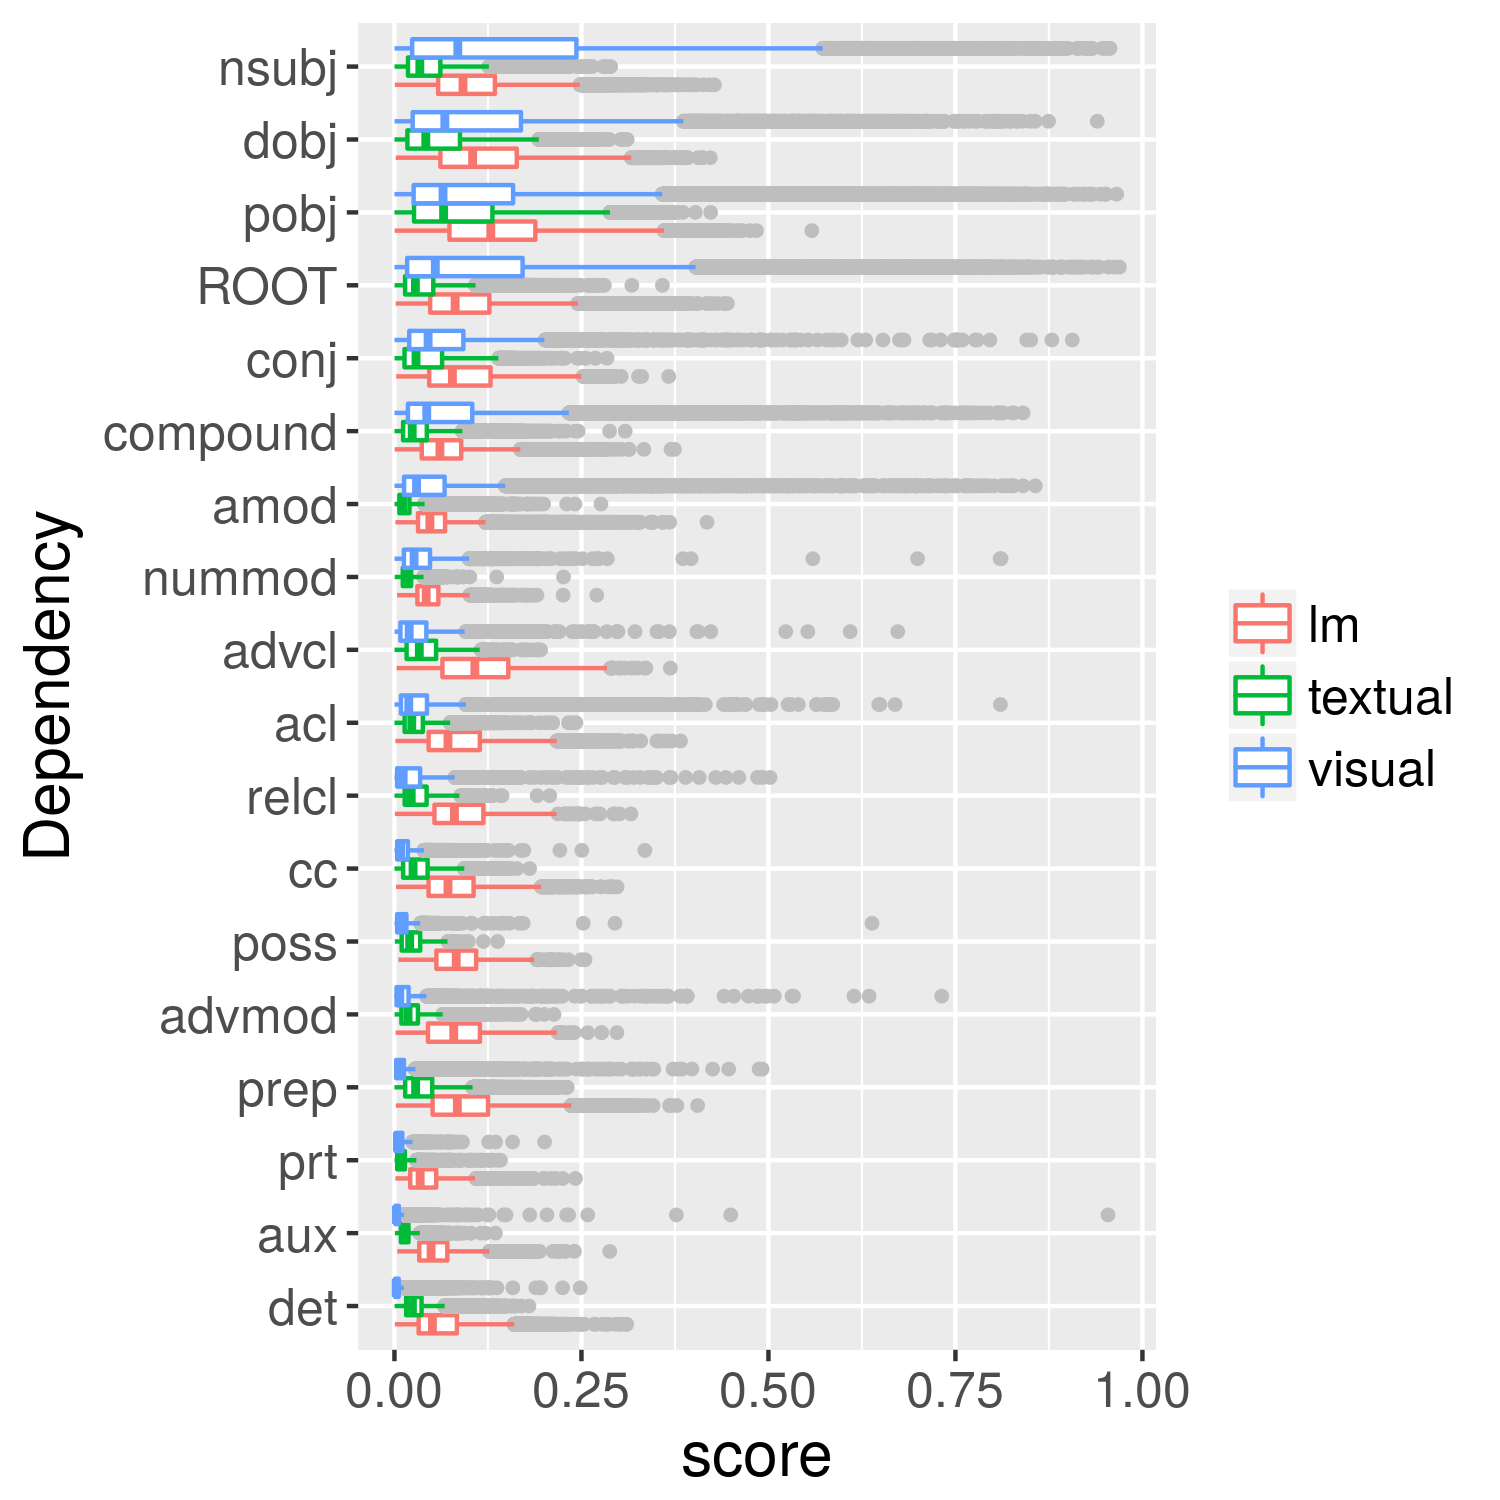
\includegraphics[scale=0.9]{imaginet-omission-dep-boxplot.png} 
%  \end{tabular}
  
\caption{Distribution of omission scores for POS (left) and dependency labels
  (right), for the {\sc Textual} and {\sc Visual} pathways and for
  {\sc LM}. Only labels which occur at least 1250 times are included.}
\label{fig:omission-imaginet}
\end{figure}

\begin{figure*}[t]
  \centering
  \hspace*{-0.2in}
  \setlength{\tabcolsep}{0pt}
  \begin{tabular}{cc}
  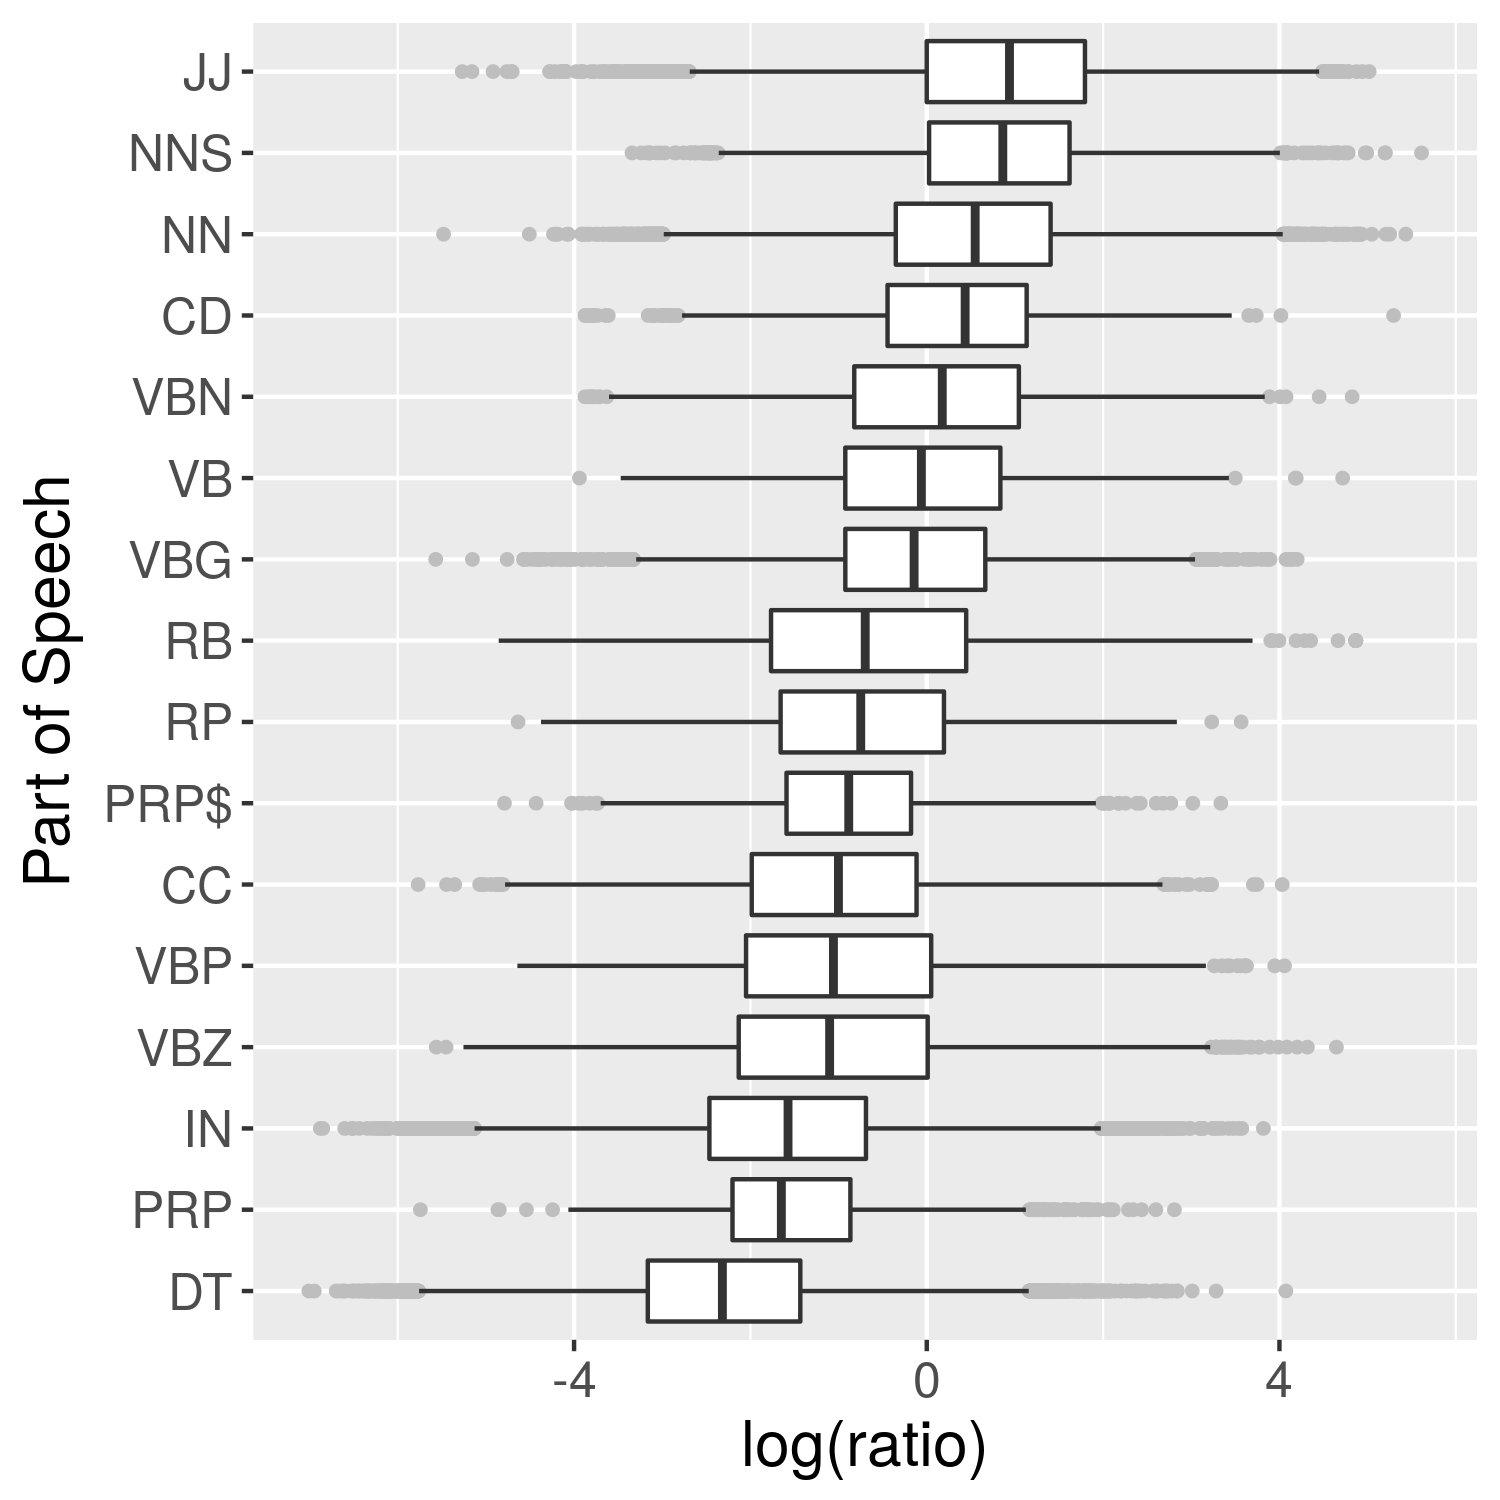
\includegraphics[scale=0.55]{imaginet-omission-ratio-pos-boxplot.png} &
  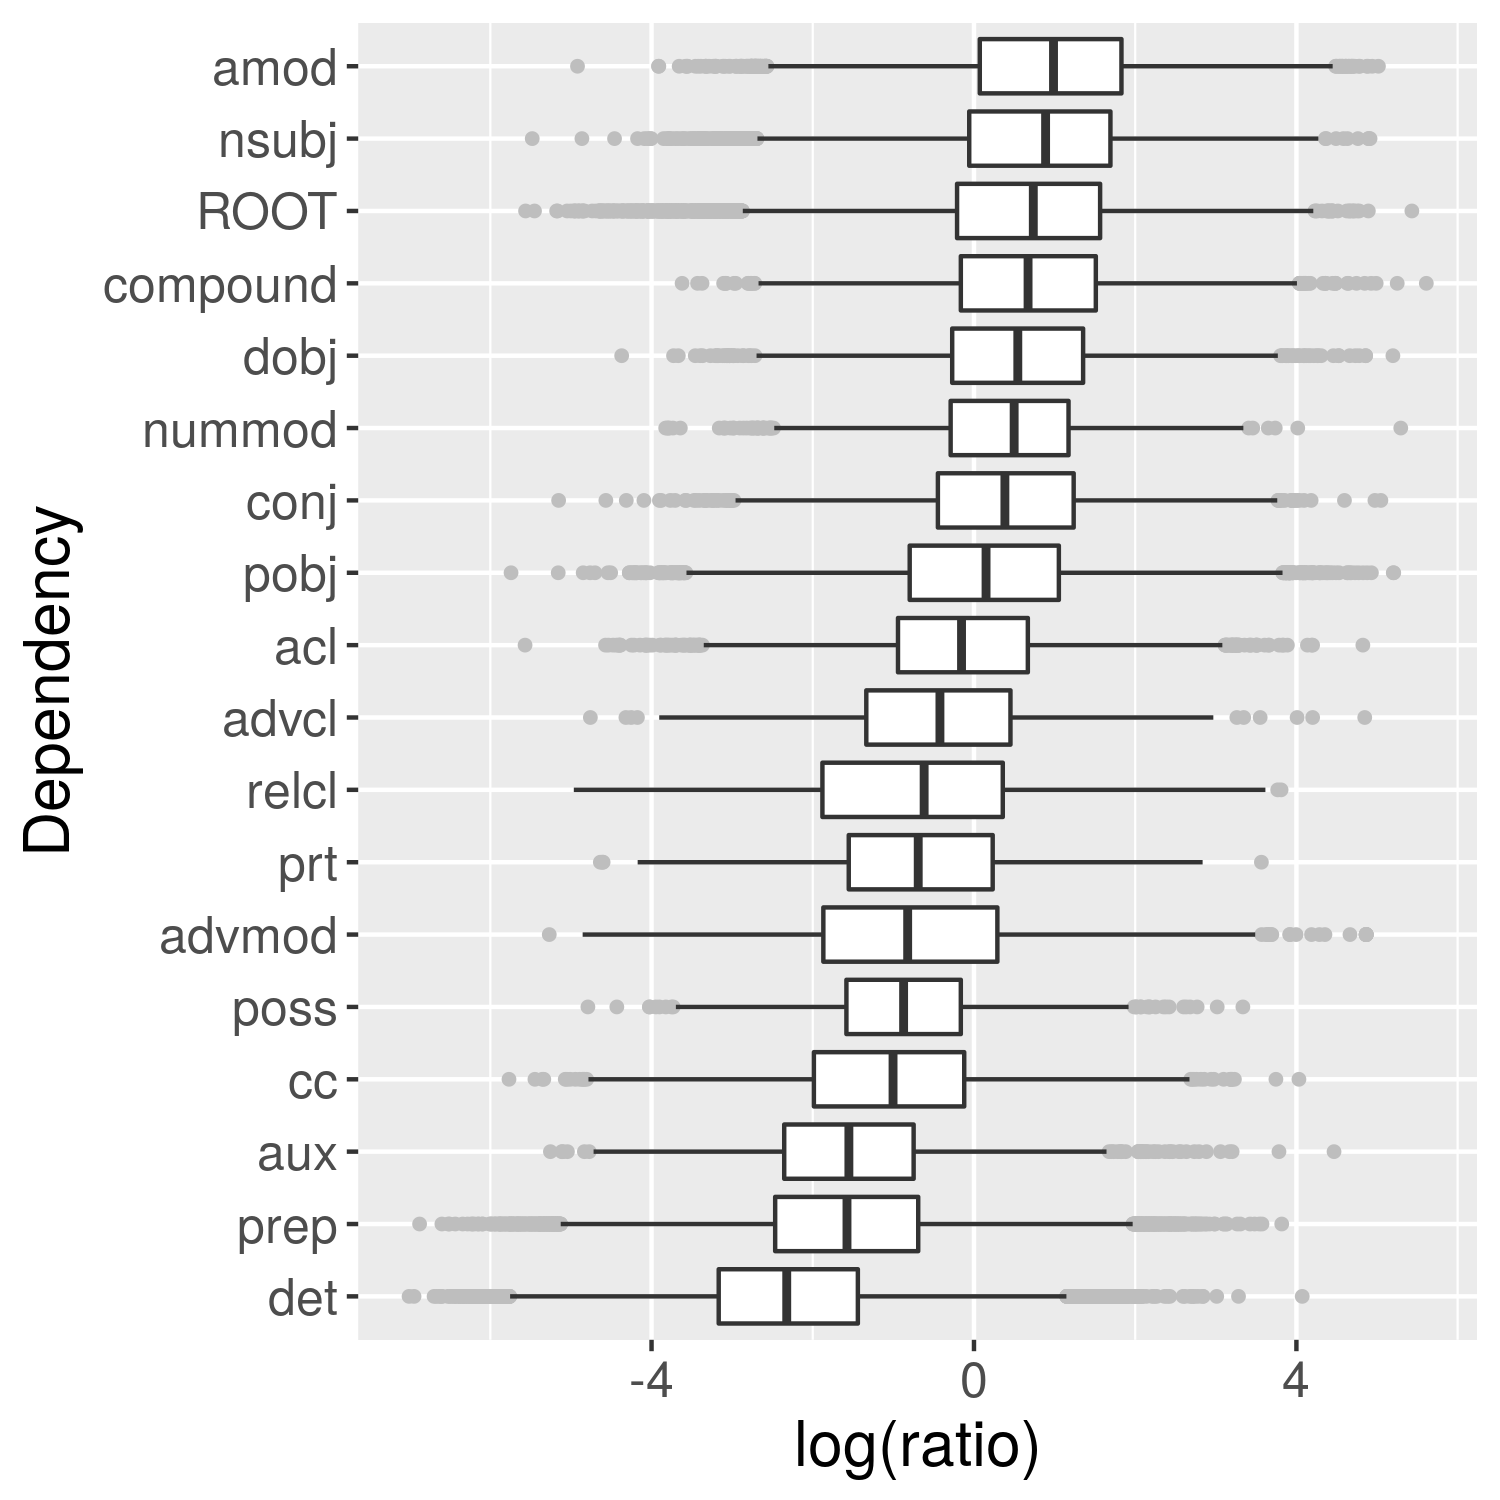
\includegraphics[scale=0.55]{imaginet-omission-ratio-dep-boxplot.png} \\  
  \end{tabular}
  \caption{Distributions of log ratios of omission scores of {\sc Textual} to {\sc Visual} per
    POS (left) and dependency labels (right). Only labels which occur at least 1250 times are included.}
\label{fig:omission-imaginet-ratio}
\end{figure*}



The omission scores can be used not only to
estimate the importance of individual words, but also of syntactic
categories. We estimate the salience of each syntactic category by
accumulating the omission scores for all words in that category. We
tag every word in a sentence with the part-of-speech (POS) category
and the dependency relation (deprel) label of its incoming arc. For
example, for the sentence \emph{the black dog}, we get ({\it
  the},~DT,~det), 
({\it black},~JJ,~amod), ({\it dog},~NN,~root). 
Both POS tagging and dependency parsing are performed 
using the  \verb+en_core_web_md+ dependency parser from the Spacy package.\footnote{Available at
  \url{https://spacy.io/}.} 
%The POS tags used are the Penn Treebank tags and the dependencies are 
%the Stanford basic dependencies.


Figure~\ref{fig:omission-imaginet} shows the distribution of omission
scores per POS and dependency label for the two pathways of {\sc
  Imaginet} and for {\sc LM}.\footnote{The boxplots in this and
  subsequent figures are Tukey boxplots and should be interpreted as follows: the box extends
from the 25th to the 75th percentile of the data; the line across the
box is the 50th percentile, while the whiskers extend past the lower
and upper quartile to $1.5\times$
the interquartile range (i.e.\ 75th percentile - 25th percentile); the
points are outliers.\label{ft:boxplots}}  The general trend is that for the {\sc
  Visual} pathway, the omission scores are high for a small subset of
labels - corresponding mostly to nouns, less so for adjectives and
even less for verbs - and low for the rest (mostly function words and
various types of verbs). For {\sc Textual} the differences
are \label{edit:textualomission} smaller, and the pathway seems to be
sensitive to the omission of most types of words.  For {\sc LM} the
distribution over categories is also relatively uniform, but the omission scores are higher
overall than for {\sc Textual}.

Figure~\ref{fig:omission-imaginet-ratio} compares the two pathways of
{\sc Imaginet} directly using the log of the ratio of the {\sc Visual}
to {\sc Textual} omission scores, and plots the distribution of this
ratio for different POS and dependency labels.  Log ratios above zero
indicate stronger association with the {\sc Visual} pathway and below
zero with the {\sc Textual} pathway. We see that in relative terms,
{\sc Visual} is more sensitive to adjectives (JJ), nouns (NNS, NN),
numerals (CD) and participles (VBN), and {\sc Textual} to determiners
(DT), pronouns (PRP), prepositions (IN) as well finite verbs
(VBZ, VBP).

This picture is complemented by the analysis of the
relative importance of dependency relations: {\sc Visual} pays most
attention to the relations {\sc amod, nsubj, root,
  compound, dobj, nummod}
whereas {\sc Textual} is more sensitive to {\sc det, prep, aux, cc, poss, advmod, prt, relcl}.
As expected, {\sc Visual} is more focused on grammatical
functions typically filled by semantically contentful words, while
{\sc Textual} distributes its attention more uniformly and 
attends relatively more to purely grammatical functions. 

It is worth noting, however, the relatively low omission scores for verbs in case \label{edit:generality}
of {\sc Visual}. One might expect that the task of image prediction from
descriptions requires general language understanding and so high omission
scores for all content words in general, however, the results
suggest that this setting is not optimal for learning useful representations of verbs,
which possibly leads to representations that are too task-specific 
and not transferable across tasks. 

\begin{figure*}[t]
  \centering
  \hspace*{-0.2in}
  \setlength{\tabcolsep}{0pt}
  \begin{tabular}{cc}
  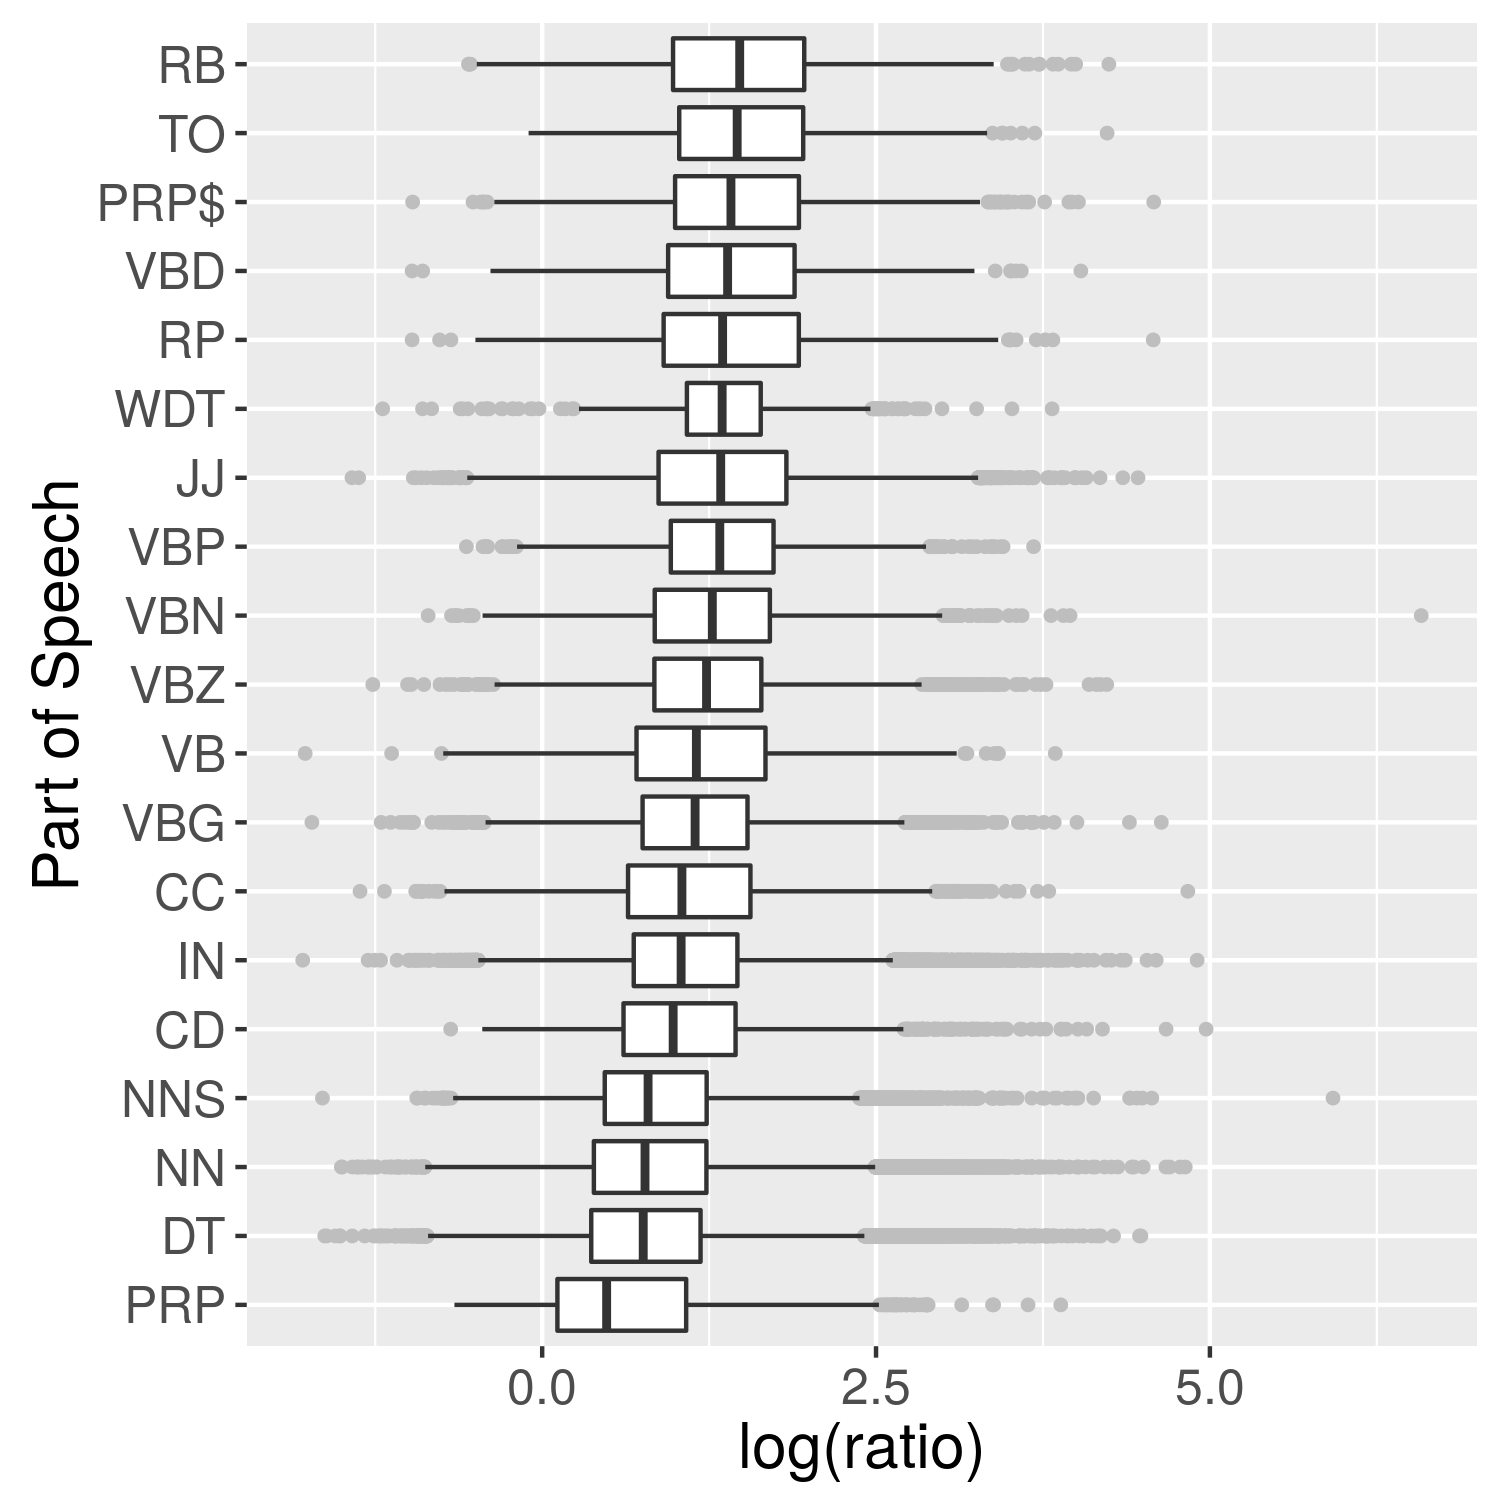
\includegraphics[scale=0.55]{imaginet-omission-quotient-pos-boxplot.png} &
  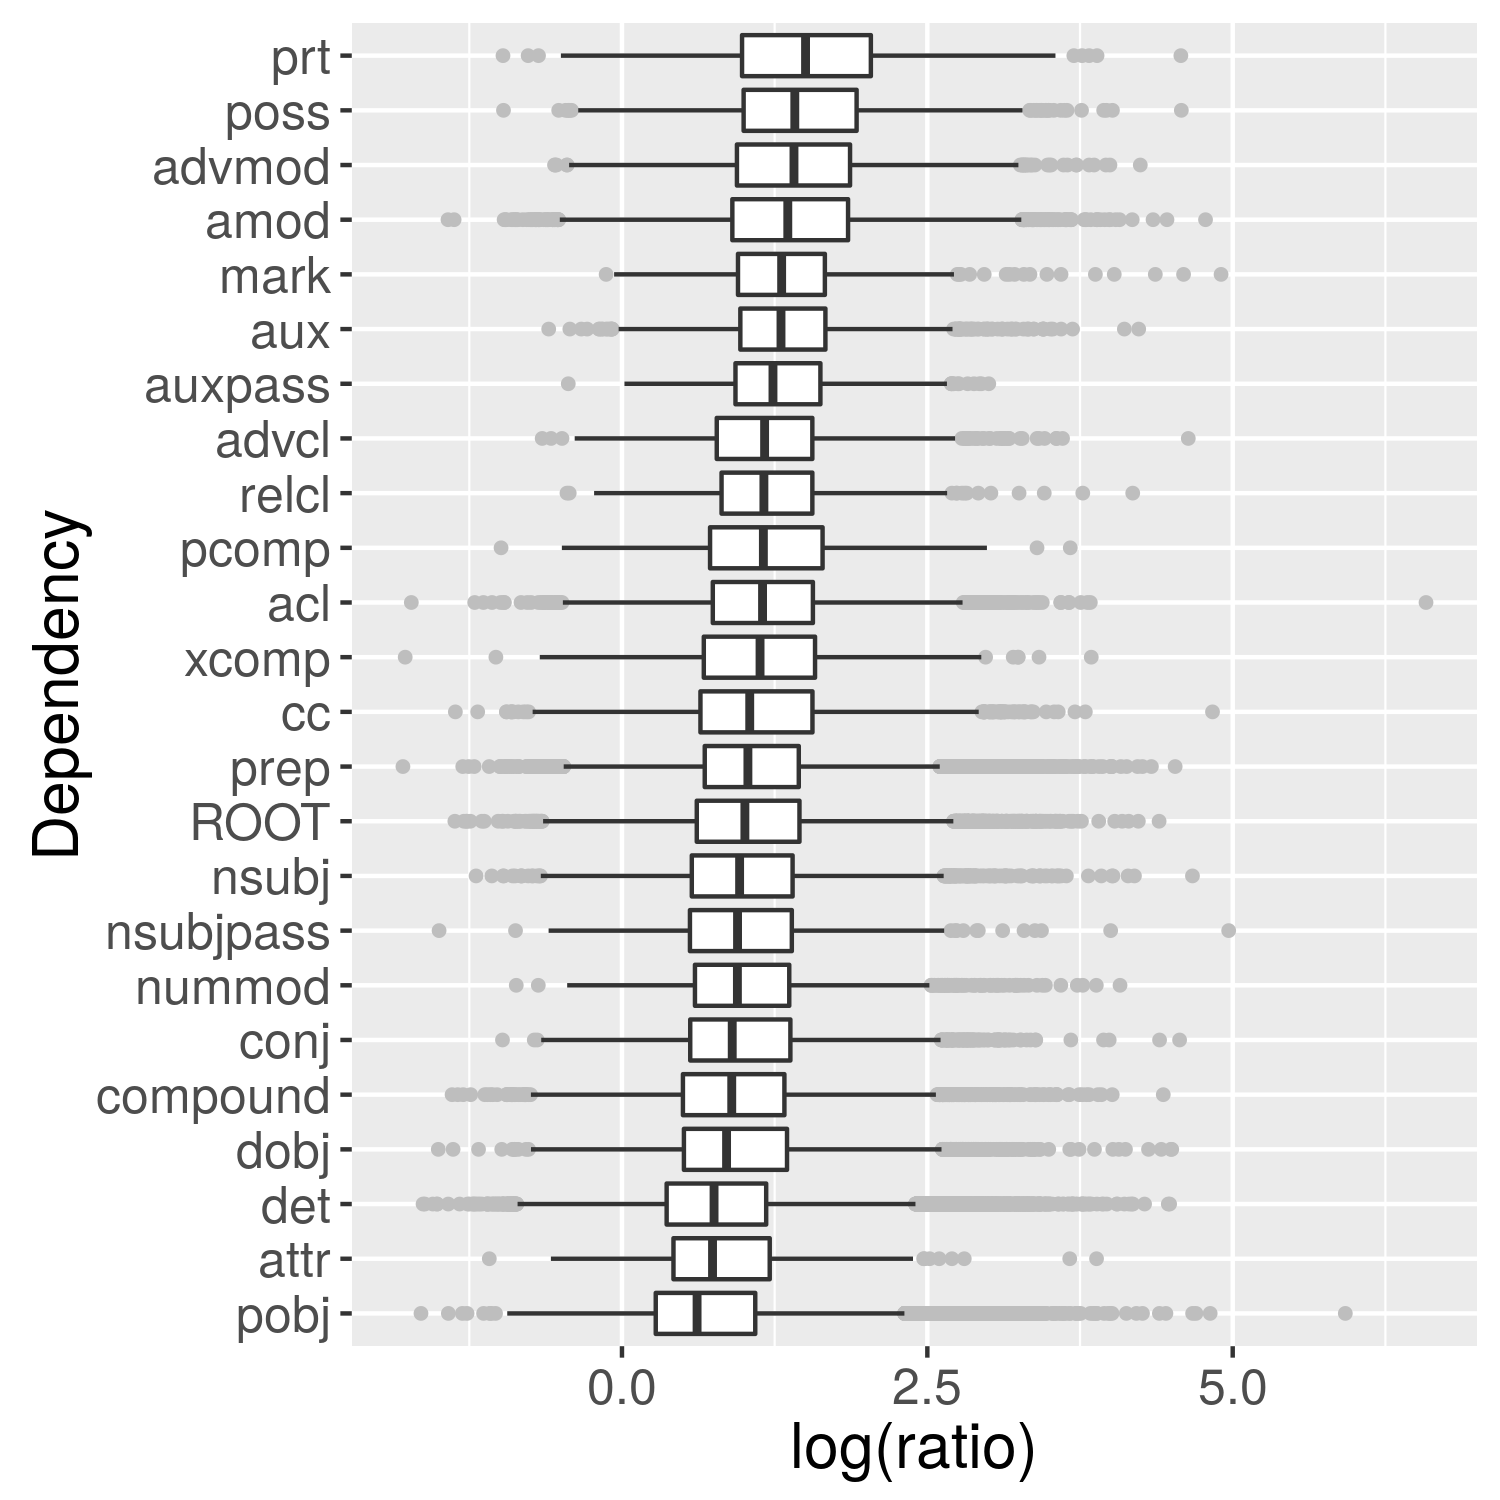
\includegraphics[scale=0.55]{imaginet-omission-quotient-dep-boxplot.png} \\  
  \end{tabular}
  \caption{Distributions of log ratios of omission scores of {\sc LM} to {\sc Textual} per
    POS (left) and dependency labels (right). Only labels which occur at least 1250times are included.}
\label{fig:omission-imaginet-quotient}
\end{figure*}


Figure~\ref{fig:omission-imaginet-quotient} shows a similar analysis
contrasting {\sc LM} with the {\sc Textual} pathway of {\sc
  Imaginet}. The first observation is that the range of values of the
log ratios is narrow, indicating that the differences between these
two networks regarding which grammatical categories they are sensitive
to is less pronounced than when comparing {\sc Visual} to {\sc
  Textual}. While the size of the effect is weak, there also seems to
be a tendency for the {\sc Textual} model to pay relatively more
attention to content and less to function words, compared to
{\sc LM}: it may be that the {\sc Visual} pathway pulls {\sc Textual}
in this direction by sharing word embeddings with it.


Most of our findings up to this point conform reasonably well to prior
expectations about effects that  particular learning objectives should
have. This fact serves to validate our methods. In the next section we
go on to investigate less straightforward patterns.

%The results on syntactic categories for {\sc Visual} are somewhat similar to 
%{\sc Sentiment} in that both models seem to learn to focus on one
%particular category (Nouns for {\sc Visual}, Adjectives for {\sc Sentiment}). 
%{\sc Visual} still incorporates adjectives, personal
%pronouns and verbs to the representations, but tends to ignore
%words of other categories. 


\subsection{Beyond Lexical Cues}
\label{sec:beyondlexical}

Models that utilize the sequential structure of language 
have the capacity to interpret the same word-type differently depending on
the context. The omission score distributions in Section \ref{sec:omitimaginet} 
show that in the case of {\sc Imaginet} the 
pathways are differentially sensitive to content vs.\ function
words. In principle, this may be either just due to purely lexical features or the model 
may actually learn to pay more attention to the same word type in appropriate
contexts. This section investigates to what extent our models
discriminate between occurrences of a given word in different positions and 
grammatical functions. 


%The analysis we described here takes
%the omission scores as input data, therefore it can be potentially applied 
%to any architecture for which the omission scores can be computed. However,
%the presented analysis and results regarding word positions can only be meaningful
%for Recurrent Neural Networks as they compute their representations sequentially and are not
%limited by fixed window sizes.\footnote{CNNs with multi-word filters
%and tree-structured recursive neural networks do not incrementally build representations
%of sentences in a left-to-right or right-to-left fashion. 
%Bi-directional RNNs, on the other hand, are sensitive by word-order and can potentially
%learn to handle the same word in different positions differently. \label{edit:foot}}

We fit four L2-penalized linear regression models which predict the omission 
scores per token with the following predictor variables: 
\begin{enumerate}
	\item {\sc LR word}: word type
	\item {\sc LR +dep}: word type, dependency label and their interaction 
	\item {\sc LR +pos}: word type, position (binned as {\sc first, second, third, middle,
	antepenult, penult, last}) and their interaction
	\item {\sc LR full}: word type, dependency label, position, word:dependency interaction, 
	word:position interaction
\end{enumerate}

\noindent We use the 5000-image portion of MSCOCO validation data for 
training and test. The captions contain about 260,000 words in total, of 
which we use 100,000 to fit the regression models. We then use the rest 
of the words to compute the proportion of variance explained by the models. 
For comparison we also use the {\sc Sum} model which composes word
embeddings via summation, and uses the same loss function as {\sc
  Visual}. This model is unable to encode information about word
order, and thus is a good baseline here as we investigate the
sensitivity of the networks to positional and structural cues.

\begin{table}
  \centering
  \caption{Proportion of variance in omission scores explained by
    linear regression.}
    \begin{tabular}{l|rrrr}
               & word   & +pos  & +dep  & full \\\hline
     {\sc Sum}       & 0.654  & 0.661 & 0.670 & 0.670 \\
     {\sc LM}        & 0.358  & 0.586 & 0.415 & 0.601 \\
     {\sc Textual}   & 0.364  & 0.703 & 0.451 & 0.715 \\
     {\sc Visual}    & 0.490  & 0.506 & 0.515 & 0.523 \\
    \end{tabular}
    \label{tab:lr-r2}
\end{table}


Table~\ref{tab:lr-r2} shows the proportion of variance $R^2$ in omission
scores explained by the linear regression with the different predictors.
The raw $R^2$ scores show that for the language models {\sc LM} and 
{\sc Textual}, the word-type predicts the omission-score to much smaller 
degree compared to {\sc Visual}. Moreover, adding information about 
either the position or the dependency labels increases the explained variance for all models. 
However, for the {\sc Textual} and {\sc LM} models the position of the word adds 
considerable amount of information. This is not surprising considering that the omission
scores are measured with respect to the final activation state, and
given the fact that in a language model the recent history is most
important for accurate prediction.

Figure~\ref{fig:rsquared} offers a different view of the data to, showing
the increase or decrease in $R^2$ for the models relative to {\sc LR~+pos} 
to emphasise the importance of syntactic structure beyond the position in the sentence.
Interestingly, for the {\sc Visual} model, dependency labels are 
more informative than linear position, hinting at the importance of syntactic 
structure beyond linear order. There is a sizeable increase in $R^2$ between 
{\sc LR~+pos} and {\sc LR~full} in the case of {\sc Visual}, suggesting that 
the omission scores for {\sc Visual} depend on the words'
grammatical function in sentences, {\it even after controlling for word
identity and linear position.}  In contrast, adding additional information on
top of lexical features in the case of {\sc Sum} increases the
explained variance only slightly, which is most likely due to the unseen words
in the held out set.   

Overall, when regressing on word identities, word position and
dependency labels, the {\sc Visual} model's omission scores are the
hardest to predict of the four models suggesting that the model may be
encoding additional structural features not captured by these predictors. 
We will look more deeply into such potential features in the following sections.

\begin{figure}
\centering
  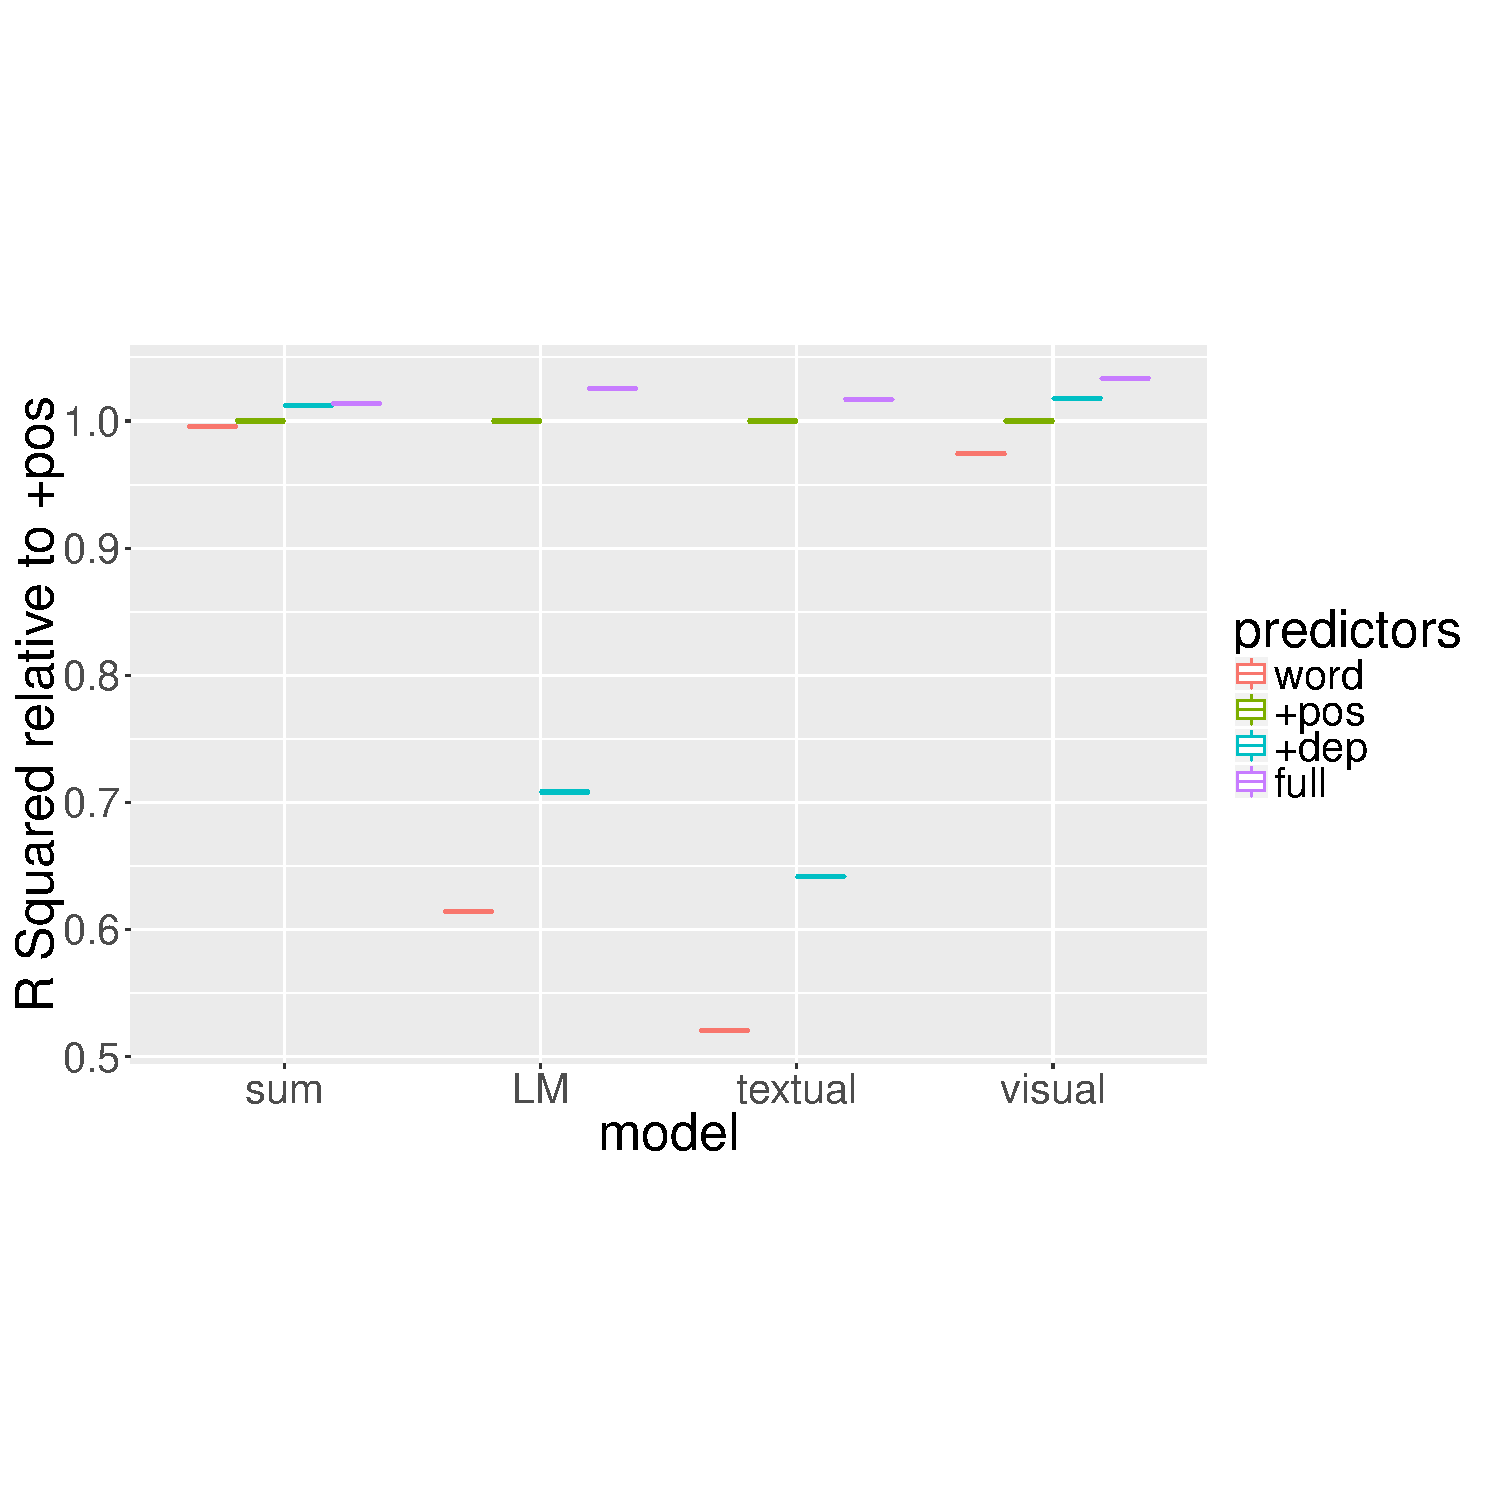
\includegraphics[scale=0.35]{position-new.pdf}
\caption{Proportion of variance in omission scores explained by the
  linear regression models
 for {\sc Sum}, {\sc LM}, {\sc Visual} and {\sc Textual}, relative to
 regressing on word identity and position only. }
\label{fig:rsquared}
\end{figure}


\subsubsection{Sensitivity to grammatical function}
\label{sec:gramfunc}

%\begin{figure}[t]
%  \centering
%  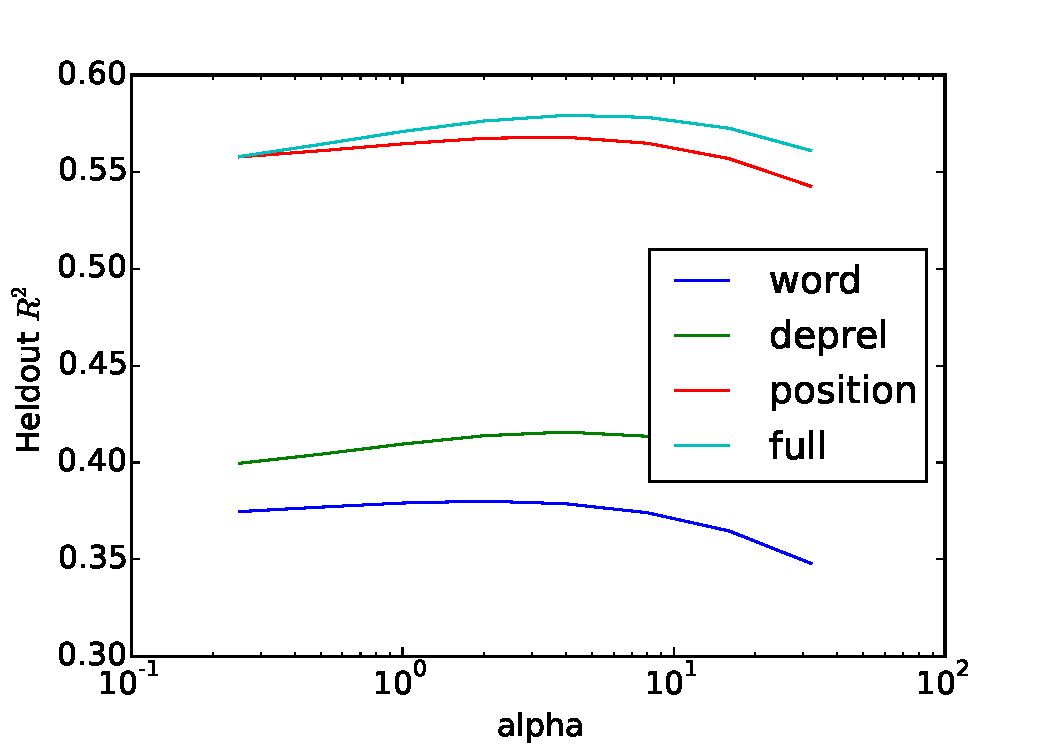
\includegraphics[scale=0.4]{omission-stat/scores-vs-alpha.pdf}
%  \caption{Proportion of variance in omission scores explained by {\sc Model 1} vs {\sc Model 2} as a function of regularization parameter $\alpha$.}
%  \label{fig:scores-vs-alpha}
%\end{figure}

\begin{figure}[t]
  \centering
  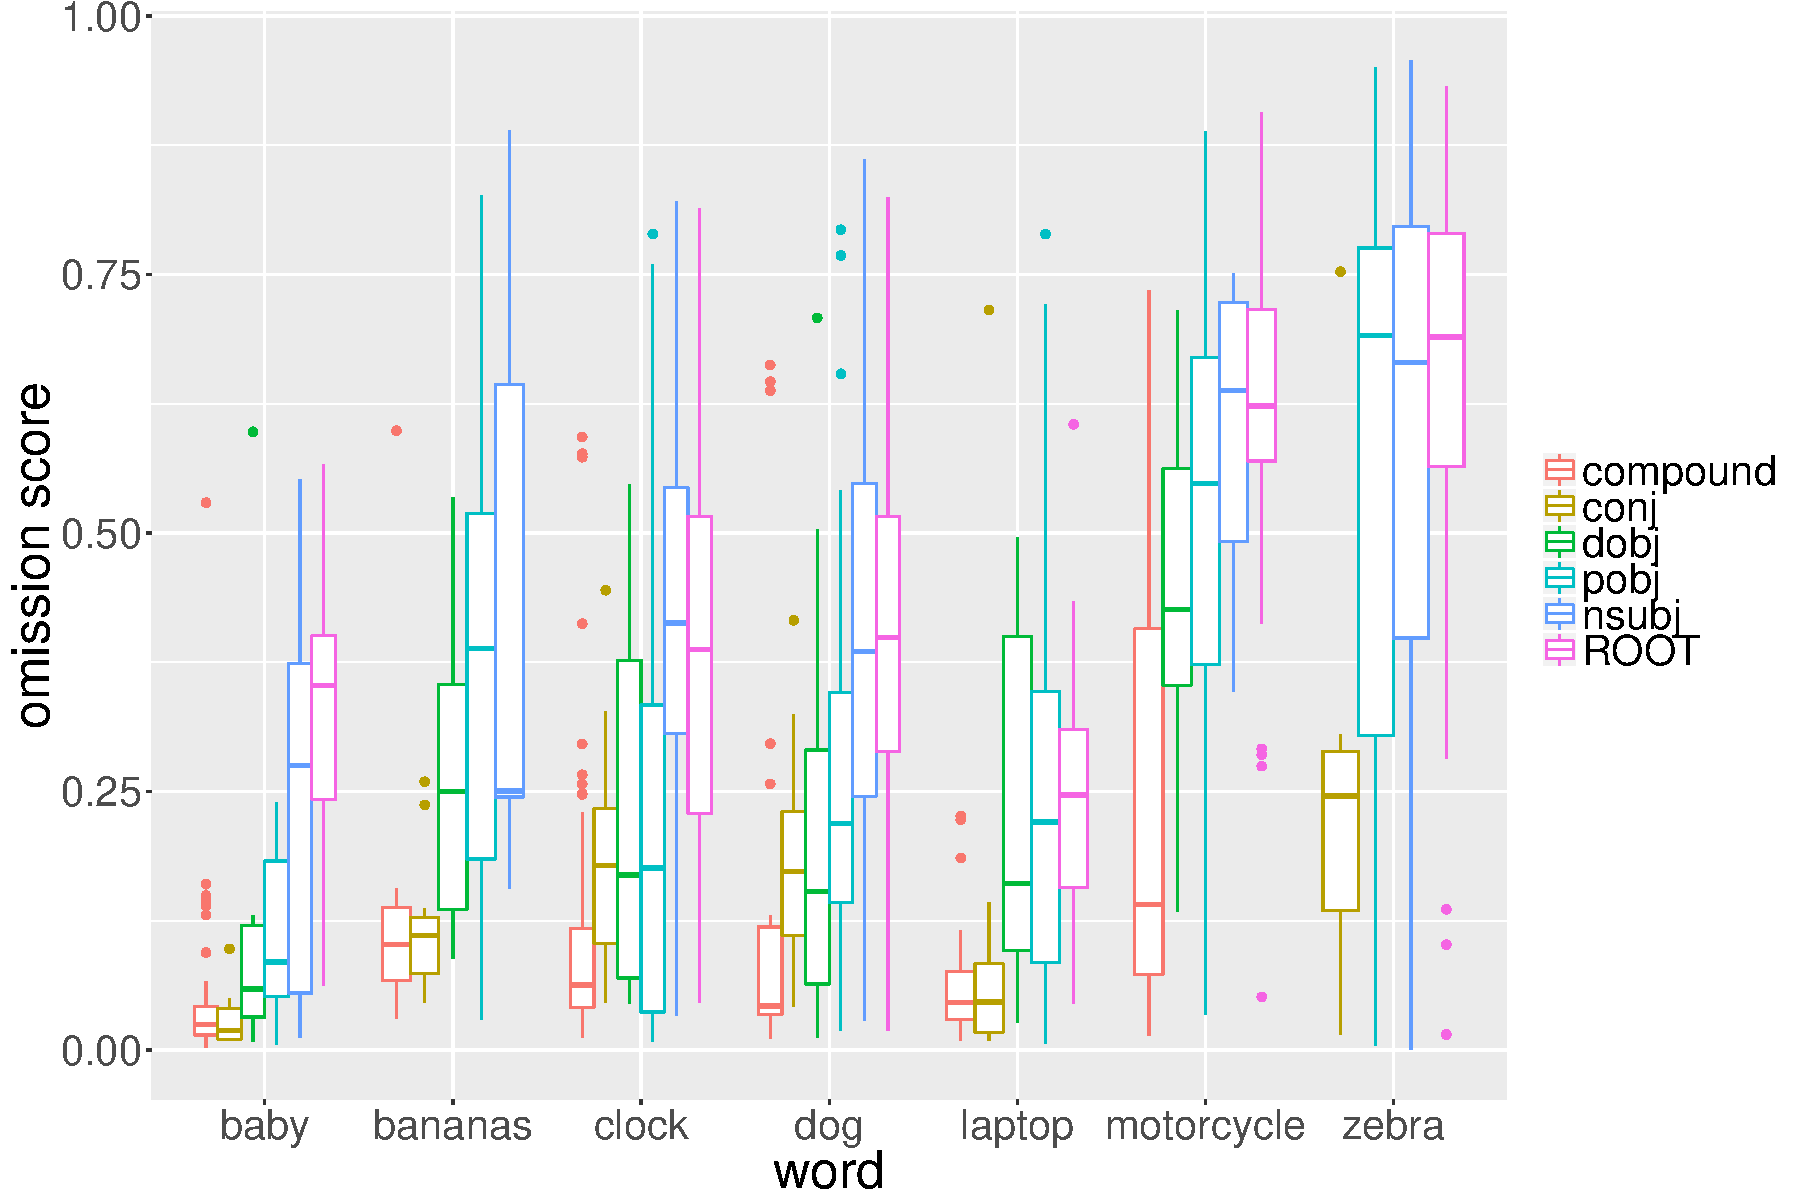
\includegraphics[scale=0.35]{top_words.pdf}
  \caption{Distribution of omission scores per deprel label for the selected word types.}
  \label{fig:top_words}
\end{figure}
%\todo{At some point redo this with words ranked by ratio between the errors not the difference}

In order to find out some of the specific syntactic configurations leading to
an increase in $R^2$ between the {\sc LR~word} and {\sc LR~+dep} predictors
in the case of {\sc Visual}, we next considered all word types with
occurrence counts of at least 100 and ranked them according to how much
better, on average, {\sc LR~+dep} predicted their omission scores 
compared to {\sc LM~word}. 

Figure~\ref{fig:top_words} shows the per-dependency 
omission score distributions for seven top-ranked words.
There are clear and large differences in how these words
impact the network's representation depending on what grammatical
function they fulfill. They all have large omission scores when they
occur as {\sc nsubj} (nominal subject) or {\sc root}, likely due to the fact that these
grammatical functions typically have a large contribution to the
complete meaning of a sentence.  Conversely, all have small omission 
scores when appearing as {\sc conj} (conjunct): this is probably because in this position
they share their contribution with the first, often more important,
member of the conjunction, for example in {\it A cow and its baby eating
  grass}. 
% The pattern for {\sc nn} (nominal modifier) is a bit more complicated: for
% four of the words shown (as well as for most other words not shown in
% the figure), the score is very low in this grammatical function--presumably 
% because most words contribute less to the sentence meaning when used  
% as modifiers than as heads (e.g.\ {\it a clock tower}). However,
% for the words {\it zebra} and {\it water}, omission scores are high
% when they act as a nominal modifier {\sc nn}. This appears due to two reasons:
% \begin{enumerate}
% \item For {\it zebra}, there are frequent erroneous parses such as {\it
%     zebra/{\sc nn} browsing/{\sc root}} instead of {\it zebra/{\sc nsubj} browsing/{\sc
%     root}}. The network does not make this mistake, and treats these
%     occurrences of {\it zebra} according to its importance as {\sc nsubj}.
% \item {\it Water} as a modifier often changes the meaning of its head in
%  a visually salient way: e.g.\ {\it water fall, water balloon, water scene, water skiing}, and
%   thus the network learns that this particular word is important in the modifier position.
% \end{enumerate}

\subsubsection{Sensitivity to linear structure}
\label{subsec:information-struct}

\begin{figure}
\centering
 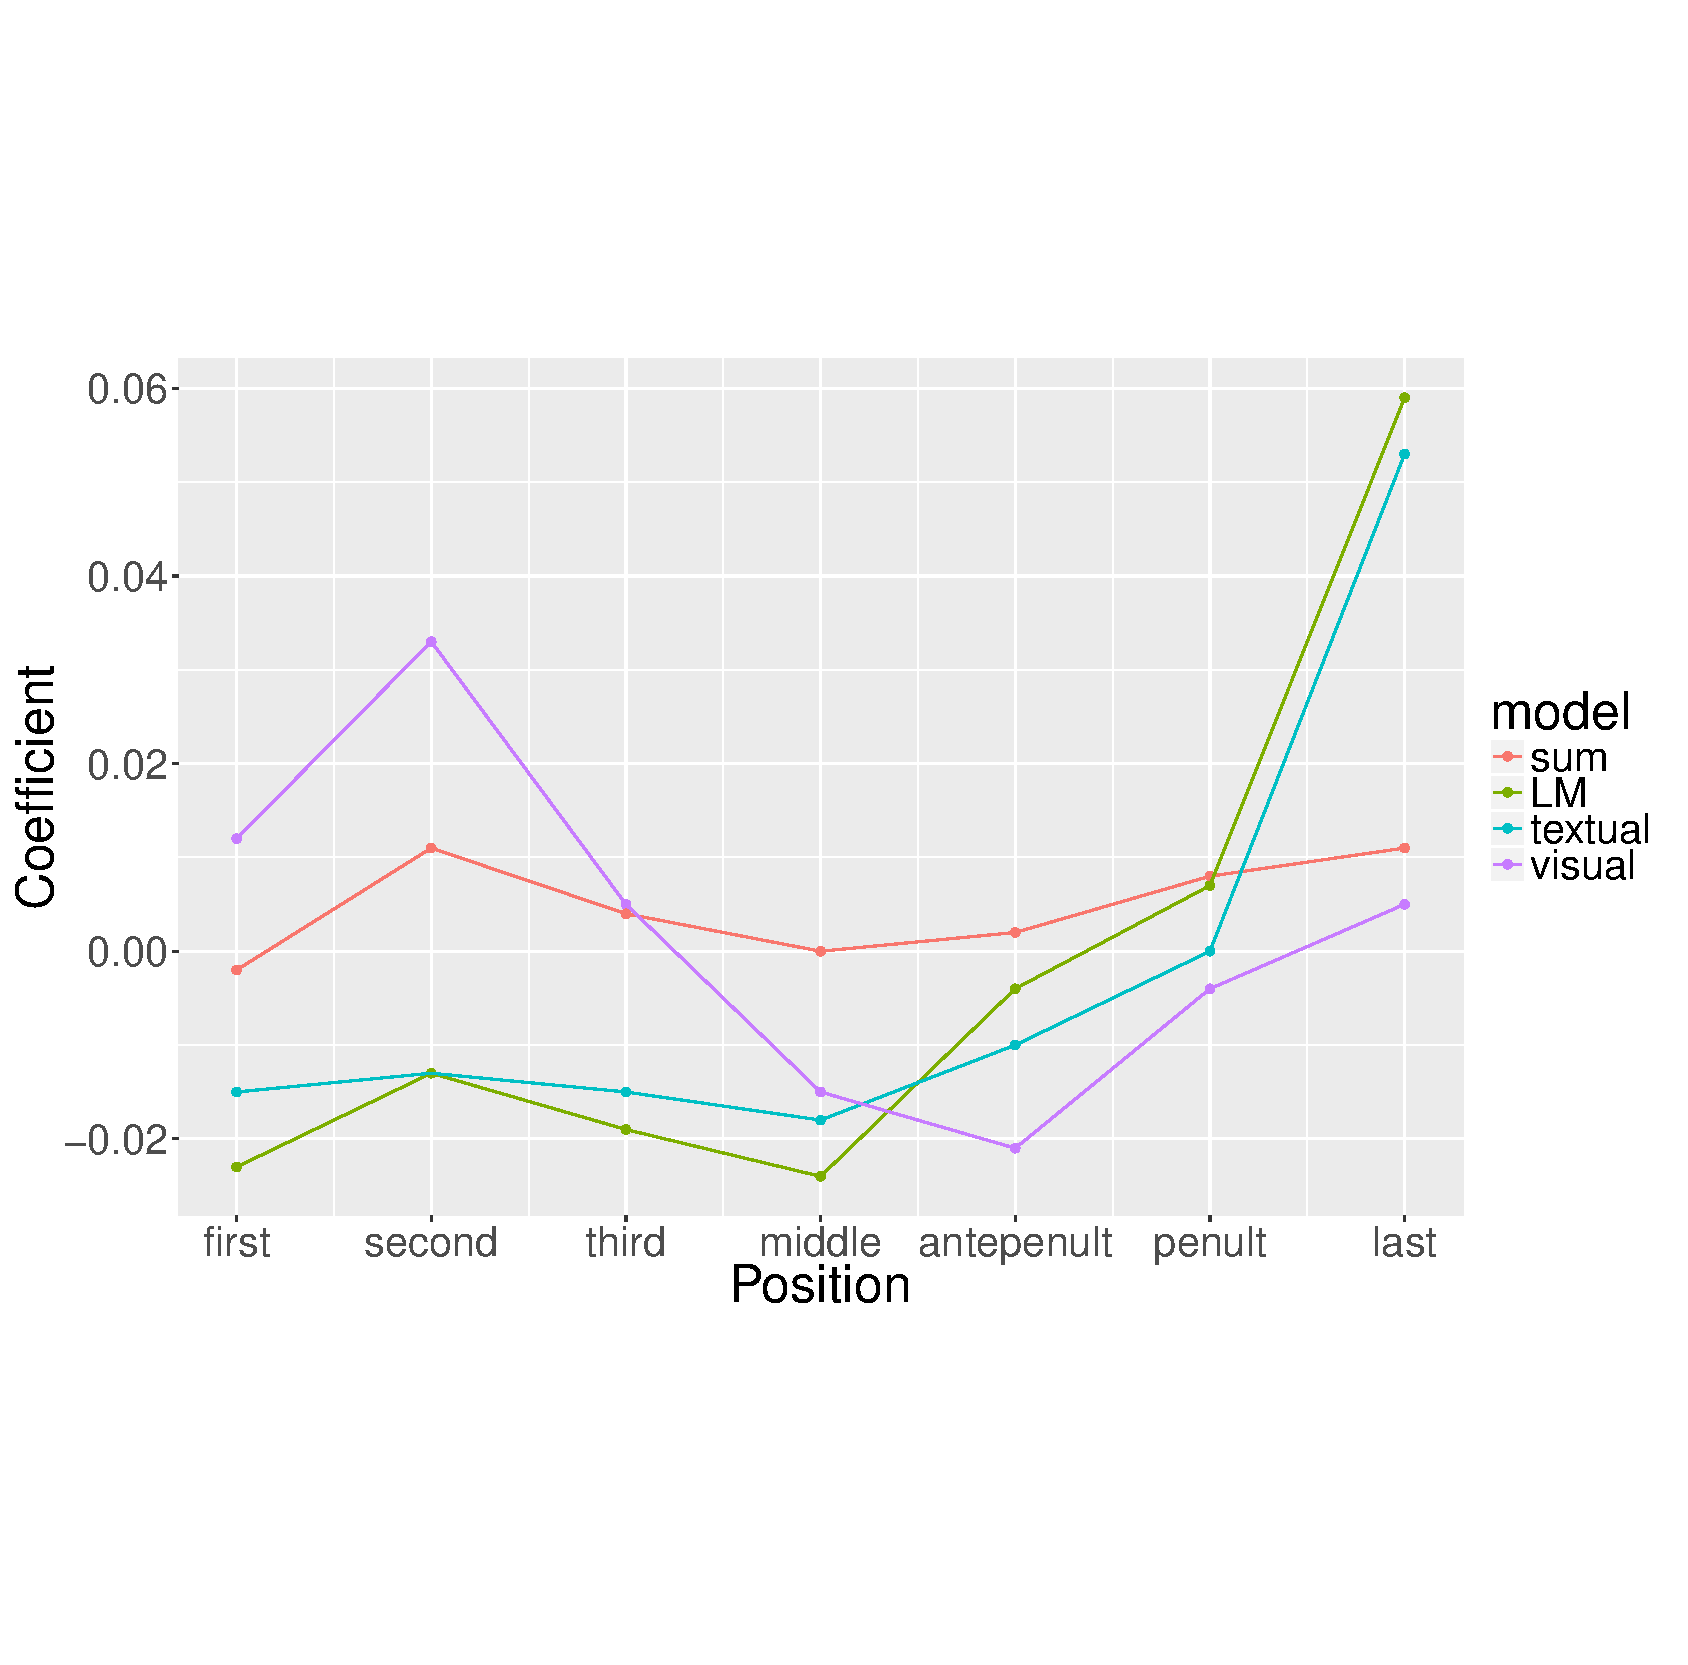
\includegraphics[scale=0.4]{position-coef.pdf}
 \caption{Coefficients on the y-axis of {\sc LR full} corresponding to the
position variables on the x-axis.}
 \label{fig:posrqs}
\end{figure}
 
As observed in Section \ref{sec:beyondlexical}, 
adding extra information about the position of words 
explains more of the variance in the case of {\sc Visual} and especially
{\sc Textual} and {\sc LM}.
Figure \ref{fig:posrqs} shows the coefficients corresponding to the
position variables in {\sc LR~full}. Since the omission scores 
are measured at the end-of-sentence token, the expectation is that 
for {\sc Textual} and {\sc LM}, as language models,  
the words appearing closer to the end of the sentence would have a
stronger effect on the omission scores. This seems to be confirmed by
the plot as the coefficients for these two networks up until the
\emph{antepenult} are all negative. 


For the {\sc Visual} model it is less clear what to
expect: on the one hand due to their chain structure,  
RNNs are better at keeping track of
short-distance rather than long-distance dependencies and thus we can expect 
tokens in positions closer to the end of the sentence to be more important. 
On the other hand in English the information structure of a single
sentence is expressed via linear ordering: the {\sc topic} of a 
sentence appears sentence-initially, and the {\sc comment} follows. 
In the context of other text types such as dialog or multi-sentence \label{edit:topiccomment}
narrative structure, we would expect {\sc comment} to often be more
important than {\sc topic} as {\sc comment} will often 
contain new information in these cases. In our setting of image captions 
however, sentences are not part of larger discourse, it is sentence
initial material that typically contains the most important 
objects depicted in the image, e.g. {\it {\underline{two zebras}} are grazing in tall grass on a savannah.}
Thus, for the task of predicting features of the visual scene, it would 
be advantageous to detect the topic of the sentence and up-weight its
importance in the final meaning representation. Figure \ref{fig:posrqs}
appears to support this hypothesis and the network does 
learn to pay more attention to  words appearing
sentence-initially. This effect seems to be to some extent mixed with the recency
bias of RNNs as perhaps indicated by the relatively high coefficient of the {\it last}
position for {\sc Visual}. 


% The basic idea is to focus on
% words which occur in several grammatical functions, and see whether
% the network treats the different occurrences differently based on the
% dependency label. 

% The omission score results for {\sc Visual}
% suggest that the model pays relatively more attention to 
% categories {\sc nsubj, pobj, root} than to {\sc nn}. 
% Since the same word types can potentially
% assume these categories in different contexts which leads to the
% hypothesis that {\sc Visual} learned to recognize small syntactic 
% constructions. In the following experiment we consider word types 
% that appear with all four of the following dependency labels: 
% {\sc nsubj, pobj, root, nn}. Table \ref{tab:nnexample} demonstrates
% examples of the systematic pattern that in when tokens with deprel {\sc nn}
% have the lowest 

% A systematic pattern that provides evidence to support
% the hypothesis is that when nouns assume the role of noun complement
% {\sc nn}, their omission score is the lowest. This result is illustrated
% in 

% \iffalse
% \subsection{Distribution of omission scores}

% Determining feature importances from RNN hidden states for NLP tasks
% allows to uncover what kinds linguistic features models focus on.  We
% showed that omission scores allow for interesting qualitative
% comparison between RNN based models, but also provides insight into
% the nature of the combinations of data sets and tasks. The omission
% score results shows that to estimate the polarity of the sentence a
% model should primarily focus on adjectives. More interestingly the
% relative higher omission scores for Nouns for {\sc Visual} suggests
% that combination of the MS-COCO data set and the pre-trained VGG-CNN
% image-representation prediction as objective does not seem to promote
% the model to learn to pay attention to verbs. This analysis suggests
% that this particular setting does not allow the model to learn general
% representations for phrases/sentences as it promotes filtering out the
% information content of verbs.  Relative to {\sc Visual} the
% omission-score distribution of the {\sc Skip-gram} is much flatter
% providing an indication that the model does not throw away as much
% important linguistic information.  \todo{show some plot of the
%   distributions VISUAL vs. skip-gram} \fi

%\section{Analysis of the function of individual hidden units}
%\label{sec:micro}
%
%\subsection{Top $K$ contexts}
%\label{sec:topk}
%
%\begin{table}[t]
%\small
%\caption{Contexts from the top 20 trigrams for example hidden units in each pathway.}
%\label{tab:contexts}
%\vspace{.2cm}
%\centering
%    \begin{tabular}{ | p{6cm} | p{6cm}|}
%    \hline
%    {\sc Visual} & {\sc Textual} \\
%    \hline
%   examples & examples  \\
%   \hline
%   \end{tabular}
%\end{table}
%
%
%The aim of this section is to develop methods that allow
%for the qualitative analysis of the kinds of linguistic features
%that individual hidden dimensions of RNNs encode. 
%We develop a simple method we dub {\it top $K$ contexts} 
%after the {\it top $K$ images} of \namecite{zhou2014object}.
%In this technique, we forward each sentence
%token by token through an RNN, and register the activation 
%of each unit in the last hidden layer of the network $\mathbf{h}_{t}$
%at each time step $t$. This results in a vector $M_i$ 
%for each hidden unit $i$, which contains  the activation of that unit 
%as a response to every token in the corpus.
%
%For each unit $i$, the entries with the highest absolute values in 
%$M_i$ represent the triggers that unit $i$ is most sensitive to. The 
%triggers could be a single token, or an n-gram including the token 
%received at the time of activation. We call such n-grams {\it top 
%contexts} of unit $i$. In this section, we analyze the top $k$ contexts
%of the hidden units to see whether they share any syntactic and/or 
%semantic patterns, indicating the function each unit is trained to perform.
%We also provide a comparison of the kinds of features the {\sc Visual} and 
%{\sc Textual} pathways of {\sc Imaginet} encode based on analysis on the 
%top $K$ contexts from the validation portion of the MS-COCO data set. 
%
%This method can be straight-forwardly applied to various 
%RNN architectures such as Elman networks or LSTMs 
%as it only requires storing the activation values for hidden units and 
%their corresponding context. For architectures with $n$ hidden layers
%one could extract multiple activation vectors $M_i^{1}, \ldots, M_i^{n}$
%for each unit, and perform analysis on each of them separately.
%A limitation of the generalizability of our analysis is that in the case of 
%bi-directional architectures the interpretation of the features
%extracted by the RNNs that process the input tokens in the reversed order
%might be hard from a linguistic point of view. 



%This involves forwarding each sentence from a corpus token-by-token through 
%an RNN, and storing the hidden activation of the network $\mathbf{h}_{t}$ 
%for each time step $t$. This results in an activation 
%matrix $M\in R^{d\times n}$, where
%$d$ is the number of hidden dimensions and $n$ is the 
%total number of time steps (or tokens) in the whole corpus. 
%Each cell $M_{it}$ in the resulting matrix represents 
%the activation value of the $i^{\text{th}}$ unit for some token at 
%time step $t$ in the corpus. 
%%Co-indexing time steps $t$ with the original sentences 
%%from the corpora allows to map the activation values of a 
%%certain neuron to a certain token in a particular context. 
%Making the assumption that high activation values indicate 
%importance, we sort the rows of the activation matrix $M$ by the 
%magnitude of the activations, leading to the top $K$ contexts for each unit.
%This method can be straight-forwardly applied to various 
%RNN architectures such as Elman networks or LSTMs 
%as it only requires storing
%the activation values for hidden units and their corresponding context.
%For architectures with $n$ hidden layers
%one could extract multiple activation matrices $M^{1}, \ldots, M^{n}$
%and perform analysis on each of them separately.
%
%In the following sections \ref{sec:topk}, \ref{sec:syntacticdim} and
%\ref{sec:carryover} we provide a qualitative exploration of the kinds of
%features the {\sc Visual} and {\sc Textual} pathways of {\sc Imaginet}
%encode based on analysis on the {\it top $K$ contexts} from the validation portion of
%the MS-COCO data set. All techniques introduced in these section can be applied
%in the same setting where {\it top $K$ contexts} can be applied.
%A limitation of the generalizability of our 
%analysis is that in the case of 
%bi-directional architectures the interpretation of the features
%extracted by the RNNs that process the input tokens in the reversed order
%might be hard from a linguistic point of view. 
%
%\subsection{Specialized hidden units}
%\label{sec:topk}
%
%Table~\ref{tab:contexts} shows the top 5 trigram contexts with the
%highest activations for five example hidden units for {\sc Visual}
%and {\sc Textual}. 
%\todo[inline]{can we explain how we chose these units, e.g. the ones with the highest maximum activation?}
%It shows the general pattern that the individual
%dimensions become highly sensitive towards contexts with syntactically
%and/or topically related patterns. 
%\todo[inline]{update the examples in Table 1 and their description below.}
%For example the top 20 trigram
%contexts for the first hidden unit of {\sc Visual} in
%Table~\ref{tab:contexts} all contain tokens topically  
%related to home electronics, such as phones, remotes and camera parts. Top-20 
%5-gram contexts for this unit include: {\it cell phone calculator and gum, 
%all hanging on wires like, such as beads and cords}. 
%
%More interestingly, the first hidden unit  for {\sc Textual} in  Table~\ref{tab:contexts}
%seems to be highly active for a combined syntactic and semantic template:
%contexts including a token corresponding to a vehicle followed by a transportation verb.
%Exploring a larger context of 5-grams reveals other interesting units 
%with high activations for such semantic/syntactic constructions in {\sc Textual}, e.g.\
%{\it a dog pokes his head, white cat sticking his head, a dog sticking its head, a dog 
%sticking his head, with a long tail perched.} 
%Further qualitative analysis on the top 50 contexts of some of the neurons {\sc Visual} shows that the model allocates certain dimensions to perform semantically informative compositions. One of the examples in Table~\ref{tab:contexts} shows that {\sc Visual} seems to learn to compose the tokens "teddy" and "bear". Another example for {\sc Visual} is a dimension, where the top context almost exclusively includes phrases with the sequence "black and white". 

%\subsection{Hidden dimensions specialized for capturing structural information}
%\label{sec:syntacticdim}
%
%Previous work \cite{} has shown during training for a specific task, that individual units (or 
%dimensions) in the hidden layers of RNNs can be specialized to capture relevant aspects of 
%information in the input. We hypothesize that some of the dimensions in the hidden layers of 
%both {\it Textual} and {\it Visual} models encode specialized structural information about the 
%utterances. 

%The aim of this section is to develop methods that allow
%for the qualitative analysis of the kinds of linguistic features
%that individual hidden dimensions of RNNs encode. 
%As discussed in the previous section, some of the analyzed units are sensitive to 
%lexical features, whereas others seem to respond to structural properties of the 
%input contexts. 

%To systematically explore the syntactic functions encoded by 
%specialized dimensions, we train two logistic regression models (one for {\sc Visual} 
%and one for {\sc Textual}) to predict the dependency label of a token at time
%step $t$. The models use two sets of predictors:
%\begin{itemize}
%  \item hidden activation vectors $\mathbf{h}_t^V$ or $\mathbf{h}_t^T$
%  \item n-gram features up to a window size of 4; for example, to predict the label 
%  for {\it dog} in the sentence {\it the nice dog}, we extract the n-gram features \{ {\it the}$_2$, {\it nice}$_1$, 
%  {\it dog}$_0$, {\it the$_2$ nice$_1$}, {\it nice$_1$ dog$_0$}, {\it the$_2$ nice$_1$ 
%  dog$_0$}\}.
%\end{itemize}
%Since the models include n-gram predictors, the logistic regression model will only
%have coefficients with high absolute values for hidden units that are predictive of 
%dependency relations over and above the n-gram features, and thus most 
%likely represent some type of functional information. Therefore, for each model 
%we pinpoint the hidden dimensions that are most predictive of each dependency label by 
%searching for the ones whose corresponding logistic regression coefficients 
%have the highest absolute value. 
%
%\begin{table}
%\small
%\caption{Examples from the top contexts for the most predictive units per dependency label in {\sc Textual} and {\sc Visual}.}
%\label{tab:syntax}
%\begin{center}
%    \begin{tabular}{|p{6cm}| p{6cm}|}
%    \hline
%   {\sc Textual} & {\sc Visual} \\
%    \hline
%    {\bf poss}:  dog sticking his, is brushing her, child brushing their, is brushing his &
%    {\bf aux}: tennis player is, racquet that is, colored ties are, but they are\\
%    \hline
%    
%    {\bf num}: several other hot, woman holding two, playing with two, group of three &
%    {\bf cc}: a waterway and, for construction or, some rocks and, with trees and\\
%    \hline
%
%    {\bf advmod}:  up a very, in a very, on a very, others watch very &
%    {\bf num}: pole in two, light with two, steeple and two, set between two\\
%    \hline
%
%   {\bf pobj}: a table covered, at a baseball, in a baseball, at a professional &
%   {\bf prep}: area surrounded by, a field with, and mountains in, the background among\\   
%       \hline
%
%   {\bf advcl}: serious while playing, standing and playing, couch while playing, as 
%he plays &
%   {\bf poss}: court holding her, player holds his, to come his, ball with her \\
%   
%   \hline
%    \end{tabular}
%\end{center}
%\end{table}
%
%
%\todo[inline]{update examples in Table 2 and their description below.}
%Table~\ref{tab:syntax} shows the top four context representations for the hidden units 
%corresponding to one of the highest coefficients for a number of the deprels for both 
%{\sc Visual} and {\sc Textual}. Some of the units in Table~\ref{tab:syntax} seem to offer 
%solely lexical cues to the deprel prediction model, while others encode more general 
%syntactic information. A number of units have high activations for target words typically 
%fulfilling the same grammatical function:
%\begin{itemize}
%    \item The example unit for the category {\sc poss} in case of {\sc Textual} has top contexts with target words {\it his, her} and {\it their}. This is also true for {\sc Visual}.
%    \item The example unit for {\sc num} for {\sc Textual} has high activations for both {\it two} and {\it three}.
%    \item The example units for {\sc cc} given for {\sc Visual} has high activations in the presence of target tokens {\it and} and {\it or}.
%    \item The contexts for the dimension of {\sc Visual} with the highest coefficient for {\sc aux} have both {\it is} and {\it are} as target tokens.
%\end{itemize}
%
%\noindent These examples, similar to the results in Section~\ref{sec:macro}, 
%highlight some of the differences between the type of linguistic 
%knowledge acquired by {\sc Textual} and {\sc Visual}. We have
%seen that {\sc Visual} learns to pay relatively more attention to contentful words
%and {\sc Textual} to words with purely grammatical function. Moreover,
%while for {\sc Textual} tokens appearing near the end of the sentence
%are more salient in general, {\sc Visual} learns to pay attention to
%sentence-initial nouns as they are likely the {\sc topic} of the sentence. 

%\subsection{Units carrying over information}
%\label{sec:carryover}
%
%Further examination of some of the highly activated units reveals dimensions
%that are predictive of deprels that require information about the
%identities or grammatical functions of previous tokens. For example,
%predictive units for {\sc pobj} in the {\sc Textual} pathway in Table~\ref{tab:syntax}
%generalize over the prepositions {\it at} and {\it in}, and contexts in the top 20 include 
%additional prepositions such as {\it around a dirt} and {\it on a grass}. But interestingly, 
%rather than being active for the prepositions themselves, all top 20 contexts belong to the 
%construction {\sc prep det pobj} where the object has to do with outdoors. 
%
%For {\sc Visual}, one of the top units for the category {\sc conj} has top contexts 
%{\it with greenery and, the table and, colored circles and, wooden furniture and, furniture 
%and a.} Given that the value of this dimension predicts the presence of a conjunct at the 
%current time step, this particular dimension seems to carry over its high activation value
%to the next time step, since all the 5 example trigrams require a
%conjunct in the next step.  This is also the case for the most predictive units of {\sc Visual} for {\sc pobj}:
%the top contexts for this unit are {\it several bunches of, with lots of, the end of, has trays 
%of} and {\it in front of}, suggesting that the information content of
%the token {\it of} must be carried over the next time step.
%
%To visually explore the phenomenon of units carrying over information through time steps, 
%we searched for interesting hidden units in {\sc Visual} using their top-20 5-gram 
%representations, and plotted their activation values through time for some example 
%captions. We only used example sentences where the activation of the hidden unit 
%was in the highest decile. Figure~\ref{fig:dimheat} shows the results.
%The first two rows are examples of \emph{lexicalized units} recognizing topically
%related words and keeping them in memory until the end of the sequence. 
%The next two rows demonstrate a hidden unit active for the multi-word expressions
%\emph{next to a} and \emph{next to an}.  The following three rows show a unit
%active for noun phrase constructions which contain a numeral followed
%by a reference to a person. 
%The last three examples show a dimension that has a modest activation for tokens of 
%category {\sc food}, but has a high activation for a following food item accompanying it in 
%the visual scene. In the very last example, the unit has a modest activation for the token 
%\emph{broccoli}, then its activation decreases for \emph{on a}. With the arrival of the token 
%\emph{plate} the activation increases again, has even higher activation for \emph{with} and 
%finally the highest for \emph{potatoes}. The top 20 5-grams for this hidden unit all contain 
%multiple food items, such as vegetables and meat with chopsticks.
%%, and compartments 
%%having fruits and vegetables such as oranges and raspberries.
%
%%Furthermore, in Section \label{sec:omitstruct} we observed 
%%that the model {\sc Visual} systematically has lower omission-scores 
%%for nouns when they have function "nn" versus when they occupy 
%%the function {\sc nsubj, pobj, dobj} or {\sc root}. 
%%The present experiment provides further evidence that {\sc Visual} 
%%recognizes "nn" as a marked grammatical function in certain contexts: some of the highest context for the top 5 coefficients for "nn" prediction involve contexts are "water fountain", "baseball player", "school bus", "wedding cake" and "traffic light". 
%
%
%
%%Another dimension in the top 5 for pobj has contexts  "attached to a, front of a, photograph of a, photo of a", where the representation of the preposition seems to be carried over two time steps.
%
%
%\begin{figure}
%\setlength{\tabcolsep}{0pt}
%\centering
%\begin{tabular}{l|r}
%
%\multirow{1}{*}{\begin{sideways}\sf tree\end{sideways}} & 
%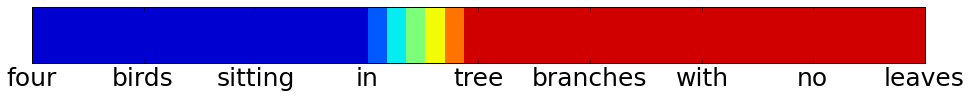
\includegraphics[scale=0.25]{dimensions/tree} \\
%\hline
%\multirow{1}{*}{\begin{sideways}\sf wii\end{sideways}} & 
% 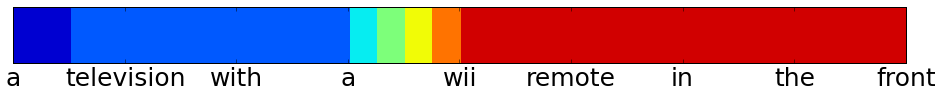
\includegraphics[scale=0.25]{dimensions/wii}  \\
%\hline
%\multirow{2}{*}{\begin{sideways}\sf next\end{sideways}} & 
%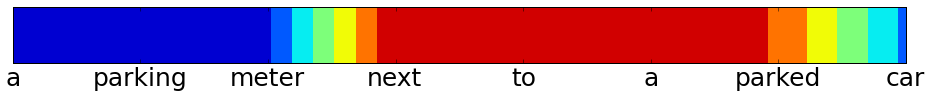
\includegraphics[scale=0.25]{dimensions/nextoacarvis} \\
%& 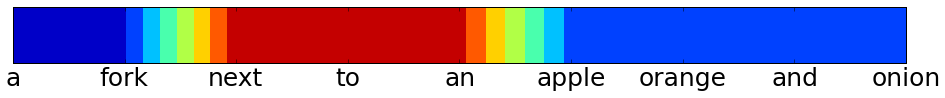
\includegraphics[scale=0.25]{dimensions/nexttoanvis}  \\
%\hline
%\hline
%\multirow{3}{*}{\begin{sideways}\sf Number\end{sideways}} & 
%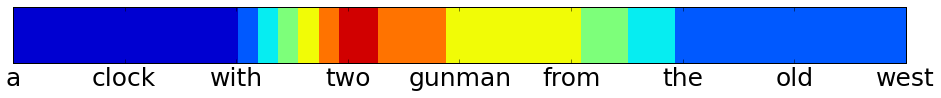
\includegraphics[scale=0.25]{dimensions/twogunmanvis}  \\
%& 
\includegraphics[scale=0.25]{dimensions/threemeneatingvis} \\
%& 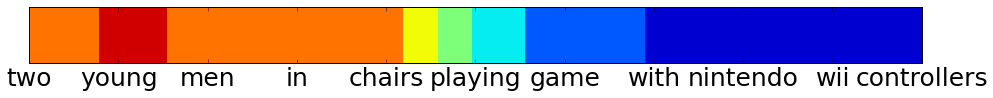
\includegraphics[scale=0.25]{dimensions/twoyoungmenvis} \\
%\hline
%\multirow{5}{*}{\begin{sideways}\sf and\end{sideways}} & 
%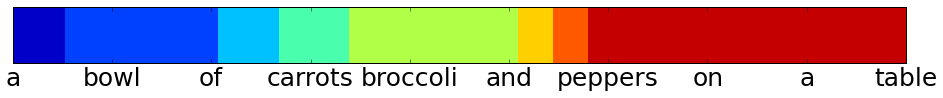
\includegraphics[scale=0.25]{dimensions/broccoliandpeppers}    \\
%& 
\includegraphics[scale=0.25]{dimensions/andgreensvis}  \\
%& 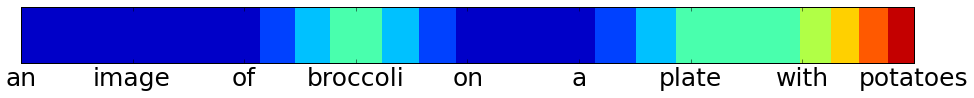
\includegraphics[scale=0.25]{dimensions/broccolipotatoes}      \\
%
%
%\end{tabular}
%
%\caption{Hidden units of {\sc Visual} active for meaningful constructions.
%The red end of the spectrum corresponds to higher activation values of the hidden unit.}
%\label{fig:dimheat}
%\end{figure}
%
\subsection{Lexical versus abstract contexts}
\label{sec:contexts}

We would like to further analyze the kinds of linguistic features that the
hidden dimensions of RNNs encode. Previous work  
\cite{karpathy2015visualizing,li2015convergent} has shown that in response 
to the task the networks are trained for, individual dimensions in the hidden layers of 
RNNs can become {\it specialised} in responding to certain types of triggers, including 
the tokens or token types at each time step, as well as the preceding context of
each token in the input sentence.
%that individual hidden dimensions of RNNs encode. 
%As discussed in the previous section, some of the analyzed units are sensitive to 
%lexical features, whereas others seem to respond to structural properties of the 
%input contexts. 

Here we perform a further comparison between the models based on the hypothesis 
that due to their different objectives, the activations of the dimensions of the last 
hidden layer of {\sc Visual} are more characterized by semantic relations within 
contexts, whereas the hidden dimensions in {\sc Textual} and {\sc LM} are 
more focused on extracting syntactic patterns. In order to quantitatively test this 
hypothesis, we measure the strength of association between activations of hidden 
dimensions and either lexical (token n-grams) or structural (dependency label n-grams) types 
of context. 

For each pathway, we define $A_i$ as a discrete random variable corresponding 
to a binned activation over time steps at hidden dimension $i$, and $C$ 
as a discrete random variable indicating the context 
(where $C$ can be of type `word trigram' or `dependency label bigram', for example). 
The strength of association between $A_i$ and $C$ can be measured 
by their mutual information:
\[
\mathrm{I}(A_i;C) = \sum_{a\in{A_i}}\sum_{c\in{C}} p(a,c)\log\left(\frac{p(a,c)}{p(a)p(c)}\right) 
\]
Similarly to \namecite{li2015convergent}, the activation value
distributions are discretized into percentile bins per dimension, such
that each bin contains 5\% of the marginal density. For context types,
we used unigrams, bigrams and trigrams of both dependency labels and
words. Figure~\ref{fig:raw_mutual} shows the distributions of the
mutual information scores for the three networks and the six context
types. Note that the scores are not easily comparable between context
types, due the different support of the distributions; they are,
however, comparable across the networks. The figure shows {\sc LM} and
{\sc Textual} as being very similar, while {\sc Visual} exhibits a
different distribution. We next compare the models' scores pairwise to
pinpoint the nature of the differences.
\begin{figure}
  \centering
  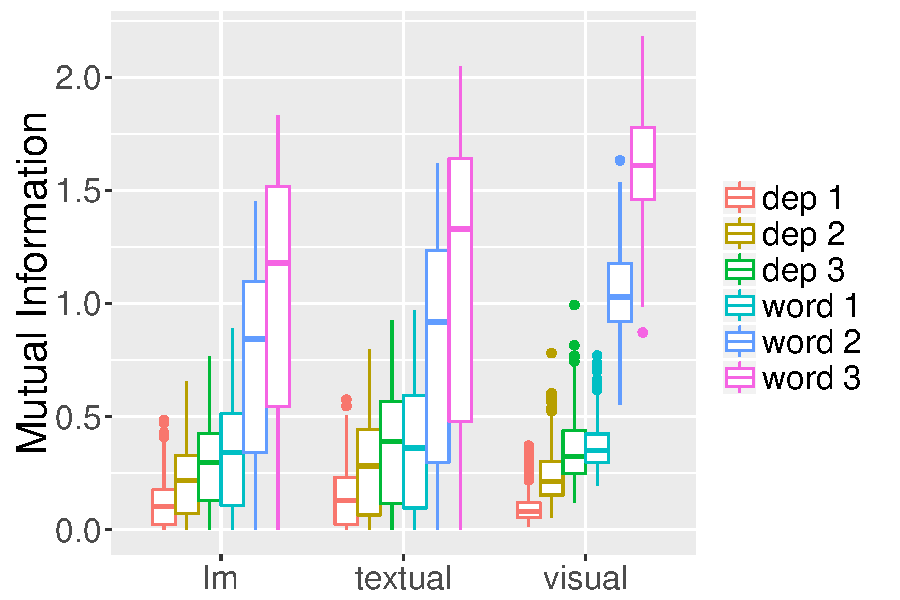
\includegraphics[scale=0.6]{raw_mutual.pdf}
  \caption{Distributions of the mutual information scores for the three networks and the six context types.}
  \label{fig:raw_mutual}
\end{figure}

We use the notation $\mathrm{MI}^\mathit{LM}_C$,  $\mathrm{MI}^T_C$ and  $\mathrm{MI}^V_C$ 
to denote the median mutual information score over all dimensions of {\sc LM}, {\sc Textual} and {\sc Visual} 
respectively, when considering context $C$. 
% We first calculate $\mathrm{MI}^{T}_{C}$ and $\mathrm{MI}^{V}_{C}$ 
% for all six context types, and observe that the median mutual information between
% activation values of the hidden units of {\sc Textual} is higher than for {\sc Visual}.
% To statistically test the observation, we used the Wilcoxon rank-sum test and performed 
% 6 pairwise comparisons between the two models. After applying Bonferroni 
% correction we found that there is a significant difference between the models in all 
% conditions ($p< 0.008$). This suggests that in general, there is a stronger 
% relationship between the activation values of the hidden units of {\sc Textual} and the 
% n-grams they co-occur with.
We then compute log ratios $\log(\mathrm{MI}^{T}_{C}/\mathrm{MI}^{V}_{C})$ and $\log(\mathrm{MI}^\mathit{LM}_{C}/\mathrm{MI}^{T}_{C})$
for all six context types $C$. In order to quantify variability we bootstrap this statistic with
5000 replicates. Figure~\ref{fig:mi-boot} shows the resulting bootstrap distributions 
for uni-, bi-, and trigram contexts, in the word and dependency conditions. 


The clear pattern is that for {\sc Textual} versus {\sc Visual}, the
log ratios are much higher in the case of the dependency contexts,
with no overlap between the bootstrap distributions. Thus, in general,
the size of the relative difference between {\sc Textual} and {\sc
  Visual} median mutual information score is much more pronounced for
dependency context types.  This suggests that features that are
encoded by the hidden dimensions of the models are indeed different, and
that the features encoded by {\sc Textual} are more associated with
syntactic constructions than in the case of {\sc Visual}. In contrast,
when comparing {\sc LM} with {\sc Textual}, the difference between
context types is much less pronounced, with distributions
overlapping. Though the difference is small, it goes in the direction
of the dimensions of the {\sc Textual} model showing higher
sensitivity towards dependency contexts.

\begin{figure}
  \centering
  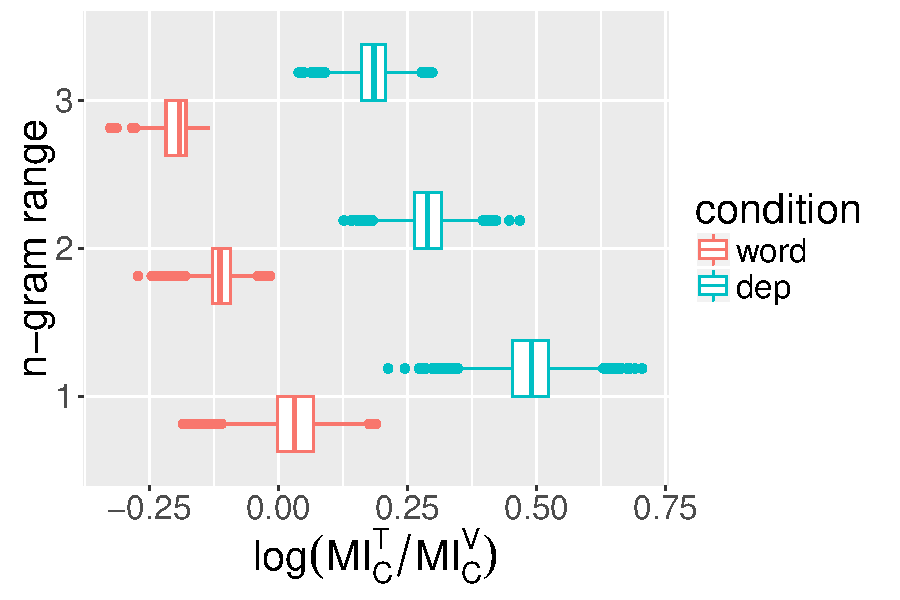
\includegraphics[scale=0.4]{bootstrappedMI.pdf}
  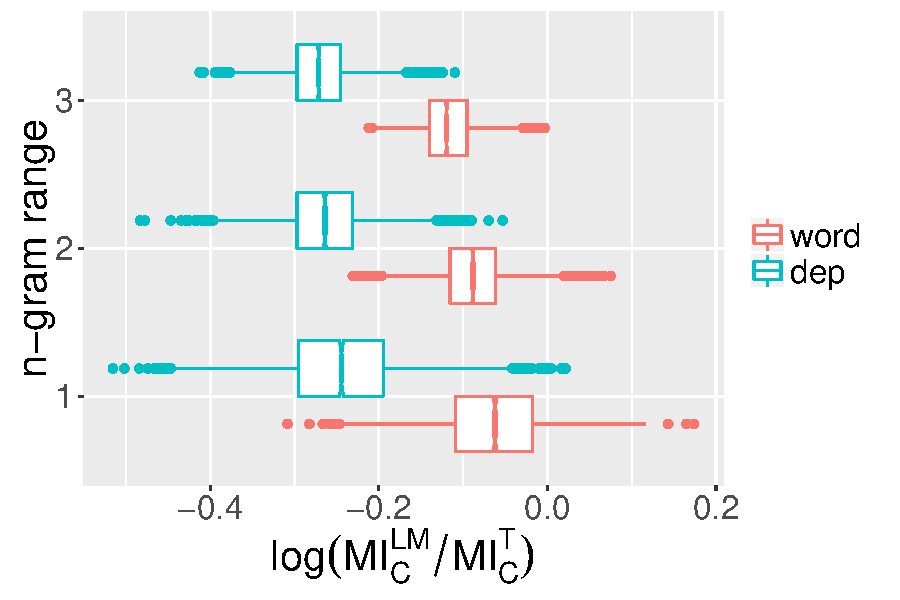
\includegraphics[scale=0.4]{bootstrappedMI2.pdf}
  \caption{Bootstrap distributions of log ratios of median mutual
    information scores for word and dependency contexts. Left: {\sc Textual}
      vs {\sc Visual}; right: {\sc LM} vs {\sc Textual}}
  \label{fig:mi-boot}
  \vspace{-.2cm}
\end{figure}


%\todo[inline]{Add and discuss sample contexts for each model here.}

The mutual information scores can be used to pinpoint specific
dimensions of the hidden activation vectors which are strongly
associated with a particular type of
context. Table~\ref{tab:mi-examples} lists for each network the
dimension with the highest mutual information score with respect to
the {\it dependency trigram} context type, together with the top
five contexts where these dimensions carry the highest value. In spite
of the quantitative difference between the networks discussed above,
the dimensions which come up top seem to be capturing something quite
similar for the three networks: (a part of) a construction with an
animate root or subject modified by a participle or a prepositional
phrase, though this is somewhat less clean-cut for the {\sc Visual}
pathway where only two out of five top context clearly conform to this
pattern.  Other interesting templates can be found by visual
inspection of the contexts where high-scoring dimensions are active;
for example, dimension 324 of {\sc LM} is high for {\it word bigram} 
contexts including
{\it people preparing, gets ready, man preparing, woman preparing,
  teenager preparing}.

\begin{table}
  \centering
  \caption{Dimensions most strongly associated with the dependency trigram context type, and the top five contexts in which these dimensions have high values.} 
\label{tab:mi-examples}
\begin{tabular}{lll}
  Network            & Dimension & Examples         \\\hline
  {\sc LM}           & 511       & cookie/pobj attached/acl to/prep \\
                     &           & people/pobj sitting/acl in/prep \\
                     &           & purses/pobj sitting/pcomp on/prep\\
                     &           & and/cc talks/conj on/prep \\
                     &           & desserts/pobj sitting/acl next/advmod \\\hline
  {\sc Textual}      & 735       & male/root on/prep a/det        \\
                     &           & person/nsubj rides/root a/det   \\
                     &           & man/root carrying/acl a/det \\
                     &           & man/root on/prep a/det         \\
                     &           & person/root on/prep a/det       \\\hline
% {\sc Textual}      & dep 3 & 1008      & bears/pobj posing/acl near/prep \\
%                    &       &           & of/prep people/pobj in/prep      \\
%                    &       &           & his/poss head/dobj on/prep       \\
%                    &       &           & food/compound dish/root with/prep    \\
%                    &       &           & living/compound room/root with/prep  \\\hline
  {\sc Visual}       &  875      & man/root riding/acl a/det \\
                     &           & man/root wearing/acl a/det \\
                     &           & is/aux wearing/conj a/det \\
                     &           & a/det post/pobj next/advmod \\
                     &           & one/nummod person/nsubj is/aux \\

% {\sc LM}           & word 3 & 38        & a professional baseball \\
%                    &        &           & rustic looking living \\
%                    &        &           & a white teddy         \\
%                    &        &           & a clean living        \\
%                    &        &           & a white beige         \\\hline
%                    % & word 3 & 117       & soccer on top \\
%                    % &        &           & ball on top \\
%                    % &        &           & frisbee on top \\
%                    % &        &           & racket playing on \\
%                    % &        &           & grazing on lush \\
% {\sc Textual}      & word 3 &  764      & down a rocky \\
%                    &        &           & on a busy \\
%                    &        &           & very busy street \\
%                    &        &           & on a busy \\
%                    &        &           & is playing tennis \\\hline
% {\sc Visual}       & word 3 & 215       & electric tooth brush \\
%                    &        &           & and a girl \\
%                    &        &           & man leans down \\
%                    &        &           & little kitty laying \\
%                    &        &           & her left hand \\

\end{tabular}
\end{table}
%Figure~\ref{fig:entropybox} shows two sets of box plots representing the mutual 
%information distributions for token and deprel n-gram contexts ($n\in{1,2,3}$). 
%Results show that in fact the medians for {\sc Textual} are higher than for {\sc Visual}, 
%especially when $C$ represents deprel n-grams. This means that {\sc Textual}
%dimensions are in fact more specialized towards reacting to syntactic contexts. 




%Motivated by the intuitively interpretable context-lists describing the function of 
%hidden dimensions using the magnitude of activations values, we turn to gain more 
%insight into the difference between TEXTUAL and VISUAL. The results in Section 
%LOGISTIC suggest that the hidden representations of TEXTUAL contain more 
%information about the syntactic structure of the input sentences than VISUAL. 
%Based on this insight we conjecture that while the activity of hidden dimensions of 
%VISUAL are characterized by semantic relationships between contexts the 
%neurons of TEXTUAL are more focused on extracting syntactic patterns. To 
%validate this assumption we consider the frequency distributions of the top 10,000 
%highest activating token and dependency relation uni-, bi- and tri-gram contexts for 
%both models. Here we make two simplifying assumptions: a) as before the 
%magnitude of the activations value suggests "importance", b) we do not take into 
%consideration the rank of the contexts. We compute the entropy of these frequency 
%distributions to measure how specialized each dimensions is to specific contexts. 
%Figure \ref{fig:entropybox} compares the distribution of entropy scores of the 
%individual hidden dimensions between TEXTUAL and VISUAL. The boxplots 
%comparing the models on dependency relations - bottom row - and tokens - top row 
%- shows that in all conditions - uni-, bi-, tri-gram - the median entropy scores for the 
%hidden dimensions VISUAL are higher than for TEXTUAL. This result suggests 
%that the features extracted from the sentences by TEXTUAL resemble syntactic 
%constructions more than in case of VISUAL. To statistically test the hypothesis we 
%use the Wilcoxon rank-sum test with and perform 6 pairwise comparisons between 
%the two models on both dependency relation and token contexts. After applying 
%Bonferroni correction we find that there is a significant difference between the 
%models in all conditions except for token bi-grams - $p< 0.05/6 = 0.008$.	

%\begin{figure*}[t]

%\begin{tabular}{ccc}
%\includegraphics[scale=0.2]{unique/MItoken1} & \includegraphics[scale=0.2]
%{unique/MItoken2} & \includegraphics[scale=0.2]{unique/MItoken3} \\
%\includegraphics[scale=0.2]{unique/MIdeprel1} & \includegraphics[scale=0.2]
%{unique/MIdeprel2} & \includegraphics[scale=0.2]{unique/MIdeprel3}
%\end{tabular}

%\caption{The distribution of the Mutual Information scores for each hidden dimension of 
%{\sc Visual} and {\sc Textual}. Plots on the top row show scores for token n-grams, and on 
%the bottom row for dependency relation n-grams.}
%\label{fig:entropybox}
%\end{figure*}




%\input{visualization}
\section{Discussion}
\label{sec:conclusion}

The goal of our paper is to propose novel methods for the 
analysis of the encoding of linguistic knowledge in RNNs trained on language tasks.
We focused on developing quantitative methods to measure the importance
of different kinds of words for the performance of such models. Furthermore, we
proposed techniques to explore what kinds of linguistic features the models
learn to exploit beyond lexical cues.

Using the {\sc Imaginet} model as our case study,
our analyses of the hidden activation patterns show that the {\sc Visual} model
learns an abstract representation of the information structure of a single
sentence in the language, and pays selective attention to lexical categories and
grammatical functions that carry semantic information. In contrast,
the language model {\sc Textual} is sensitive to features of a more
syntactic nature. We have also shown that each network contains
specialized units which are tuned to both lexical and structural
patterns that are useful for the task at hand.  


\subsection{Generalizing to other architectures}

%{\bf From 4.1 (computing omission scores):}

For other RNN architectures such as LSTMs \label{edit:omitgeneral}
and their bi-directional variants, measuring the contribution
of tokens to their predictions (or the omission scores)
can be straight-forwardly computed using their hidden state 
at the last time step used for prediction. Furthermore, the technique 
can be applied in general to other architectures which
map variable-length linguistic expressions to the same fixed dimensional
space and perform predictions based on these embeddings. 
This includes tree-structured Recursive Neural Network models such as the Tree-LSTM
introduced in \namecite{kai2015treelstm}, or the CNN architecture of \namecite{yoonneural2014} 
for sentence classification. 
%In both cases the pre-softmax activations can be extracted 
%from the models as the representations of the full and partial sentences.   
%{\bf From 4.3 (beyond lexical cues):}
However,
the presented analysis and results regarding word positions can only be meaningful
for Recurrent Neural Networks as they compute their representations sequentially and are not
limited by fixed window sizes.
% \footnote{CNNs with multi-word filters
% and tree-structured recursive neural networks do not incrementally build representations
% of sentences in a left-to-right or right-to-left fashion. 
% Bi-directional RNNs, on the other hand, are sensitive by word-order and can potentially
% learn to handle the same word in different positions differently. \label{edit:foot}}

%{\bf From old 6 (top-k-context), not sure if it's applicable to the mutual information measure:}
% This method can be straight-forwardly applied to various 
% RNN architectures such as Elman networks or LSTMs 
% as it only requires storing the activation values for hidden units and 
% their corresponding context. For architectures with $n$ hidden layers
% one could extract multiple activation vectors $M_i^{1}, \ldots, M_i^{n}$
% for each unit, and perform analysis on each of them separately.
% A limitation of the generalizability of our analysis is that in the case of 
% bi-directional architectures the interpretation of the features
% extracted by the RNNs that process the input tokens in the reversed order
% might be hard from a linguistic point of view. 

A limitation of the generalizability of our 
analysis is that in the case of 
bi-directional architectures, the interpretation of the features
extracted by the RNNs that process the input tokens in the reversed order
might be hard from a linguistic point of view. 

\subsection{Future directions}

In future we would like to apply the techniques introduced in this paper 
to analyze the encoding of linguistic form and function of 
recurrent neural models trained on different objectives, 
such as neural machine translation systems
\cite{sutskever2014sequence} or the purely distributional
sentence embedding system of \namecite{kiros2015skip}. A number of
recurrent neural models rely on a so-called attention mechanism, first
introduced by \namecite{bahdanau2014neural} under the name of soft
alignment. In these networks attention is explicitly represented, and it
would be interesting to see how our method of discovering implicit
attention, the omission score, compares. For future work we also propose to
collect data where humans assess the importance of each word in a sentence
and explore the relationship between omission scores for various models
and human annotations.\label{edit:humanjudgement} Finally, one of the benefits
of understanding how linguistic form and function is represented in RNNs is that
it can provide insight into how to improve systems. We plan to draw on
lessons learned from our analyses in order to develop models with better 
general-purpose sentence representations.




% \iffalse
% We developed \emph{macro} and \emph{micro} level methods to analyze the 
% activation patterns of Recurrent Neural Networks
% from a linguistic point of view. On the \emph{macro} level
% we introduced the $\mathrm{omission}$ score
% to measure the salience of tokens in sentences and
% showed how aggregating these scores in terms of part-of-speech categories and
% grammatical functions allows for a more in-depth understanding of the kinds of
% linguistic structure RNNs learn from linguistic data. In particular we have shown
% that {\sc Visual} learns to pay attention to tokens depending of their grammatical
% function. In these experiments we focused on how the model interprets
% the same \emph{nouns} fulfilling different grammatical functions, but in future work 
% this method can be straight-forwardly applied to other classes of content-words 
% such as \emph{verbs} or \emph{adjectives}. In addition we provided evidence 
% that {\sc Visual} pays more attention to nouns that are closer to 
% the beginning of the sentence, which is motivated by the information structure of English.
% In our \emph{micro} level analyses we developed a simple and general purpose method
% dubbed \emph{top K contexts}, which describes the function of a particular hidden unit 
% by ranking the contexts that produce the highest activation values for that unit.
% We performed exploratory analysis on these contexts, especially focusing on 
% hidden units whose activations are predictive of the grammatical function of tokens.
% We observed that in numerous cases units are highly activated for contexts that represent
% combined syntactic semantic templates. Furthermore, we explored dimensions that
% carry over their activations to represent longer term dependencies and demonstrated 
% a visualization technique to explore these patterns. Lastly, we performed a comparison
% between {\sc Textual} and {\sc Visual} using the mutual information between the activation
% values of their hidden units and the contexts. Our analysis showed a high level difference
% between the kinds of features the two pathways extract, in that the
% linguistic regularities encoded by hidden units of {\sc Textual} 
% seem to be more characterized by syntactic templates than in case of {\sc Visual}.
% In addition to the insights provided by the methods implemented in this paper
% we believe them to be general enough to allow  cognitive linguistics research 
% to further explore the linguistic knowledge in the activation patterns
% of RNNs trained on large scale data sets and on challenging tasks.

% \fi



\bibliographystyle{fullname}
\bibliography{refs}

\newpage
\pagenumbering{roman}

\noindent
Dear Dr.~Merlo,
\newline

Thank you for the very helpful suggestions and insightful questions
posed in this review.  We apologize for the delay getting this
revision back to you and very much appreciate the extension you 
gave us to resubmit the manuscript.

We have substantially revised the article in response to your and the reviewers' 
comments. Specifically with regard to the two main issues you raised, we have 
introduced a uni-modal language model (referred to as the {\sc LM} model in the text) 
and reported the results of all the experiments on this model as well. Also following 
your recommendation, we have removed the exploratory parts of (the old) Section 6, 
and reorganized the paper by merging previous Sections 4, 5 and the remaining of 
Section 6 into a single section containing all the experiments (that is Section 4 in the 
revised manuscript). We have kept and expanded the quantitative analysis of the nature of 
n-gram contexts that trigger individual dimensions in the hidden layers; this experiment is 
now reported in Section~\ref{sec:contexts}.

Furthermore, we have made clarifications about the details of the techniques all 
through the manuscript, expanded Introduction (Section~\ref{sec:intro}) to 
emphasise our contributions, updated Related Work (Section~\ref{sec:related}) 
to include relevant papers that came out while this manuscript was under review, and expanded Discussion (Section~\ref{sec:conclusion}) to discuss in more detail the relevance and generalizability of our techniques. 

We believe that the revisions to the paper address your collective
concerns, and we thank you all again for the comments that have helped
us to improve the paper.
\newline

\noindent
Sincerely,
\newline

\noindent
Ákos Kádár, Grzegorz Chrupała and Afra Alishahi
\newline


\begin{verbatim}
Dear Ákos Kádár:

We have reached a decision regarding your submission to Computational
Linguistics, "Representation of linguistic form and function in
recurrent neural networks". I include here the reviews for your
perusal.

The reviewers and I like the area of work in which this paper is
situated: model analysis. While the reviews correctly point out that
several shortcomings remain, a discussion has identified the
modifications that we think are really required, to make the paper
stronger. Other ideas are suggestions that we leave to you for future
work.

The requested changes concern an added comparisons to unimodal models
(or at least to unimodal versions of Imaginet). On the other hand, all
the reviewers thought that Section 6 is less convincing than the rest
of the paper, at least in the current writeup. So we think that this
Section could be reduced in favor of adding the unimodal experiments .

I would be grateful if you could provide an appropriately revised
version of your paper by 10th February 2017. Please email the
editorial assistant (editorialoffice@cljournal.org) within one week,
to confirm whether you will be able to meet this target date, or to
negotiate a new target date.

You will find details of the resubmission process at
http://cljournal.org/ojs-help.html.  When you submit your revised
paper, please enclose a letter that responds specifically to each of
the points made by the reviewers, outlining the changes you have made,
and those you have not addressed, together with an electronic copy of
the revised manuscript as a PDF file.

Thank you for submitting to Computational Linguistics.


Paola Merlo
University of Geneva
Paola.Merlo@unige.ch
------------------------------------------------------
Reviewer A:


2 What is this paper about? [Help] :
The paper presents methodologies for analyzing what is learned by
recurrent neural networks. It does this by suggesting two
methodologies, and then applying them to two similar tasks -- one that
that is based on language modeling, and another which is based on
visual recognition. The analysis highlights some of the things that
are encoded and not encoded in each of the representations.


3 Strengths and Weaknesses [Help]

Strengths:

The topic of understanding what is learned by neural network models,
in particular recurrent ones, is of great importance and interest, and
papers of this kind are very much needed. While most work tries to use
"deep learning" and RNNs to "improve" on various language tasks,
understanding their capabilities and inner working, and making them
more transparent, is much more challenging, and there are not enough
works in this area. The current work attempts to do precisely that,
and it also delivers on its promise with an interesting methodology
and insights. In particular, the first part (section 5) is
particularly well done. Section 6 is somewhat less convincing, but
still is on-par or better than any other work that attempts to deliver
analysis and insights.


Weaknesses:
 
Some parts of the papers were not clear, and could be improved. I also
have someissues with some of the experiments in section 6, which can
either be presented better or even removed altogether, in my view.

- In terms of clarity, I would appreciate a better description of the
  IMAGINET model, which is being analyzed. The model is described in
  terms of its equations, but I would like to see a better
  presentation of what is the intent behind it -

- what is being modeled and what is being learned? this is available
  in the original IMAGINET paper, but I think the description should
  be imported to this paper also, in order to make it self contained
  and stronger.
  
\end{verbatim}  
\begin{quote}
\textsc{Author Response:}
We have expanded Section~\ref{sec:imaginet} with a conceptual
description of {\sc Imaginet} and its learning goals, and added a graphical
representation of the structure of the model for more clarity (Figure~\ref{fig:imaginet}).
\end{quote}
\begin{verbatim}

- Also in terms of clarity, the graphs are not described in enough
  detail in my view. Whiel the box plots (figure 2 and others) are
  somewhat standard, they are not mainstream in the NLP commuity, and
  I would appreciate seeing a more detailed description in the main
  text or the caption of what each component means, both generally and
  in the context of the specific graph.
\end{verbatim}  
\begin{quote}
\textsc{Author Response:}  \todo[inline]{explain the updated graph}
\end{quote}
\begin{verbatim}
- Figure 7 is confusing -- what are the different colors between,
  e.g., the words "in" and "tree" in the first line, and between "a"
  and "wii" in the second? I assume this is some "gradient" between
  two colors, but it looks like there are several data points and is
  very confusing. Please fix this.
\end{verbatim}  
\begin{quote}
\textsc{Author Response:}  Following the recommendation of the reviewers,
we shortened the original Section 6 and removed this figure.
\end{quote}
\begin{verbatim}

In terms of content:

- In section 6.1, why is the sorting by magnitude and not by absolute
  value? are negative activations not important?
\end{verbatim}  
\begin{quote}
\textsc{Author Response:}  It was in fact the absolute value of the activations 
that was taken into account. In the revised manuscript, we have removed this 
and other exploratory experiments and expanded the quantitative analyses.
\end{quote}
\begin{verbatim}

- When choosing the "top k context of each unit" (section 6.1), it is
  not clear what a "unit" is and how it is chosen.
\end{verbatim}  
\begin{quote}
\textsc{Author Response:}  A unit is one individual dimension in the final hidden layer 
of the network. We have made this clear in the revised text.
\end{quote}
\begin{verbatim}

- I did not understand the last sentence in section 6.1, and would
  appreciate an elaboration on this point (or a removal).
\end{verbatim}  
\begin{quote}
\textsc{Author Response:}  We removed this part and added an expanded discussion of the generalizability of our techniques to Discussion (Section~\ref{sec:conclusion}).
\end{quote}
\begin{verbatim}

- In section 6.2, it is not clear how trigrams with high activations
  are chosen. How is a trigram with high activation defined? this is
  not clear from the description of the method.
\end{verbatim}  
\begin{quote}
\textsc{Author Response:} We have removed this section in the revised manuscript. We 
address the nature of contexts which trigger individual dimensions and a systematic
procedure for selecting the dimensions themselves in more detail now in 
Section~\ref{sec:contexts}.
\end{quote}
\begin{verbatim}

- I am not convinced by the experiments in section 6.3 and their
  importance -- either they are not described properly and I missed
  something, or they are somewhat meaningless: when training a
  logistic regression model to predict grammatical function, it is not
  surprising that ones finds units that are predictive of grammatical
  function.
\end{verbatim}  
\begin{quote}
\textsc{Author Response:}  As mentioned before, we have reorganised 
the experiments and remove the exploratory parts, including the old Section 6.3. 
We address the issue of encoding grammatical functions in the revised manuscript in 
Sections ~\ref{sec:beyondlexical} (specifically in \ref{sec:gramfunc}).
\end{quote}
\begin{verbatim}


~ Where is section 6.4?

\end{verbatim}  
\begin{quote}
\textsc{Author Response:} It was there, believe us! But we have removed this 
experiment from the revised version for the sake of clarity and coherence of our analyses.
\end{quote}
\begin{verbatim}

~ a related (unpublished, but available on arxiv) work is
https://arxiv.org/abs/1608.04207

\end{verbatim}  
\begin{quote}
\textsc{Author Response:}  We have expanded the discussion of related work 
(Section~\ref{sec:related}) and included this work in addition to a few others which 
came out while our submission was under review.
\end{quote}
\begin{verbatim}

4 Substantive Revisions Required [Help]

Complete this section if either 'Revise and Resubmit' or 'Reject' has
been recommended.

Revisions to be Required:
: 



Revisions to be Encouraged:
: 



5 Minor Revisions Required [Help]
:

See the points marked with (-) in the weaknesses above. Points marked
with (~) are less important. For section 6.3, my recommendation is
that it is either substantially revised, or removed altogether -- I
believe the paper has enough merit without it.

\end{verbatim}  
\begin{quote}
\textsc{Author Response:}  We hope we have addressed all your comments and concerns. We have removed the experiments in (the old) Section 6.3 from the revised manuscript.
\end{quote}
\begin{verbatim}

6 Typographic Errors [Help]
:

- "by as" in the first sentence of the intro.

- There are some cases of using parenthesis in citation where they
  shouldn't be, for example the first two citations in section 2 ("of
  (Elman 1990)" should be "of Elman (1990)").

\end{verbatim}  
\begin{quote}
\textsc{Author Response:} The typo and the citation inconsistencies are fixed.
\end{quote}
\begin{verbatim}

------------------------------------------------------

------------------------------------------------------
Reviewer E:


2 What is this paper about? [Help]
: 

The paper presents a set of methods for analyzing the activations of
recurrent neural networks from a linguistic perspective using:

a) omission scores (to examine the contribution of a single token to
the prediction of the network); and

b) top k contexts (keeping the activations for the entire sequence and
examining individual dimensions)

The model used in this paper is a multimodal (text and visual)
multi-task RNN (Imaginet). At each time step the next word is
predicted from its current state, and an image vector is predicted
from the model's final state. The model consists of two parallel GRUs
with shared word embeddings.

By pairing omission scores with POS and dependency relations, the
authors show that the Visual pathway mostly focuses on noun and noun
relations, while the textual pathway focuses more on function
words. The textual pathway has in general a more uniform omission
score distribution, the visual model peaks on content words (albeit
not particularly on verbs, as the authors discuss).


3 Strengths and Weaknesses [Help]

Strengths:
: 
* neat idea and novel contribution (pairing activations with POS and
dependency relations to gain further insights into RNNs)

* extensive analysis; especially going beyond lexical cues (Section
5.3), where the authors train a regression model to predict omission
scores on a token level, showing that the network not just learns to
rely on word types, but it also learns position information
(particularly important for the textual pathway)


Weaknesses:
: 
* the description of the top K contexts is not clear, how are top k
contexts calculated? do you find the most active token (highest
absolute value of hidden activation in the sequence?) and then use
the words around it to find the trigrams? (what is meant by 'each
unit' in Section6.1? Is the matrix actually R^nxd?); maybe you sort
by column, not row? 

\end{verbatim}  
\begin{quote}
\textsc{Author Response:}  You are absolutely right about the description of 
top k contexts being confusing. We have removed this part and reorganized 
the experiments section (Section~\ref{sec:experiments}) to make it more understandable
and coherent. 
\end{quote}
\begin{verbatim}

* Section 6.5 shows that the visual pathway focuses more on dependency
relations, supporting the finding in the omission score part;
however, the section is again very dense and Figure 7 only shows
activations for Visual; I'd suggest to drop this part from the paper

\end{verbatim}  
\begin{quote}
\textsc{Author Response:}  Following your and others' suggestion, we have removed this section from the revised manuscript.
\end{quote}
\begin{verbatim}

4 Substantive Revisions Required [Help]

Complete this section if either 'Revise and Resubmit' or 'Reject' has
been recommended.

Revisions to be Required:
: 
- clearer description of how top k contexts are obtained
\end{verbatim}  
\begin{quote}
\textsc{Author Response:}  As mentioned above, we have removed this part and reorganized Section~\ref{sec:experiments} to make our analyses more concrete and clear.
\end{quote}
\begin{verbatim}


Revisions to be Encouraged:
: 
- figures are not readable in BW printing; in addition to color, use
  different symbols/line types
\end{verbatim}  
\begin{quote}
\textsc{Author Response:}  We have reformatted many of our figures to make them more readable.
\end{quote}
\begin{verbatim}

- Related Work: clarify better how you differ from Li et al. (2015),
  you mention "for a comparative analysis": I interpret this as "we
  analyze a multi-task learning model (visual / textual) and compare
  what the two parts learn"
\end{verbatim}  
\begin{quote}
\textsc{Author Response:} We have edited our related work section to make the comparison more 
clear. In addition to taking into account tasks that rely on different modalities (language as well as vision), 
we focus more on learning structural properties of the input, whereas Li et al. (2015) focus on single
tokens.
\end{quote}
\begin{verbatim}


5 Minor Revisions Required [Help]
: 
- Sec 2, clarify: what are 'negative strings'? (non-words?)
\end{verbatim}  
\begin{quote}
\textsc{Author Response:}  we have reworded `positive' and `negative' as `grammatical' 
and `ungrammatical' to avoid confusion.
\end{quote}
\begin{verbatim}
- Before equation 9 missing lambda ("weighted by \lambda"; what lambda
  is used in the exp.?)
\end{verbatim}  
\begin{quote}
\textsc{Author Response:}  There was no $\lambda$ in that equation, but in 
Section~\ref{sec:imaginet} we report the value we use for the parameter 
$\alpha$ in Equation~(\ref{eq:losscombo}).
\end{quote}
\begin{verbatim}
- it would be helpful to include a figure of model (as in original
  paper)
\end{verbatim}  
\begin{quote}
\textsc{Author Response:}  We have included an illustration of the structure of the 
model in Figure~\ref{fig:imaginet}.
\end{quote}
\begin{verbatim}
- "two minor modifications" but the first seems you also use cosine,
  was that different previously, not clear.
\end{verbatim}  
\begin{quote}
\textsc{Author Response:}  You are right, the description of the model in 
Section~\ref{sec:imaginet} presents the version used in this paper, which uses 
cosine distance. The original Imaginet model uses mean square error instead; 
we clarified this issue in footnote~\ref{ft:imaginet}.  
\end{quote}
\begin{verbatim}
- specify interaction features in regression model
\end{verbatim}  
\begin{quote}
\textsc{Author Response:}  We have specified the interaction features used in each regression model in Section~\ref{sec:beyondlexical}.
\end{quote}
\begin{verbatim}
- 5.3.1. why also 'water'?
\end{verbatim}  
\begin{quote}
\textsc{Author Response:}  We have removed {\it water} from the set of examples 
in Figure~\ref{fig:top_words}.
\end{quote}
\begin{verbatim}


6 Typographic Errors [Help]
: 
- abstract: sentence "Based on.." way too long
- mention multi-task in abstract
- introduction: "this includes various" > "This can be applied to
  various"
- from linguistic point (missing det)
- generally avoid long sentences (e.g., last paragraph sec 5.1,
  sec. 5.2)
- rephrase: "this model we refer to as SUM"
- windowsizes
\end{verbatim}  
\begin{quote}
\textsc{Author Response:}  We have fixed these issues, thanks for bringing them to our attention.
\end{quote}
\begin{verbatim}

------------------------------------------------------

------------------------------------------------------
Reviewer F:


2 What is this paper about? [Help]
: 
This paper presents an analysis of the information learned by
recurrent neural networks. It focuses on one particular multimodal,
multitask model, Imaginet, which is trained on images and their
descriptions. The paper proposes a new measure, the omission score,
which indicates how sensitive the network is to individual words in
the input. Using this method, the authors show that the textual module
of the model pays attention to function words, while the visual module
pays attention to content words. The authors then propose a second
method which can be used to analyze which n-grams the hidden units of
the model are sensitive to; this results in meaningful syntactic and
semantic clusters. This time, there is no clear-cut distinction
between textual and visual modules.


3 Strengths and Weaknesses [Help]

Strengths:
: 
This paper makes a useful methodological contribution by proposing
methods to analyze the knowledge learned by neural networks, which is
an underexplored area, at least for networks trained on text data. The
paper is well written, and technically sound.


Weaknesses:
: 
The results of the paper are unfortunately fairly obvious. From the
omission score analysis, we learn that a model trained to predict the
next word in a sentence is sensitive to function words, while a word
trained to associate a sentence with an image representation (which is
essentially the output of the object detector) pays more attention to
nouns. This is not at all surprising, it just reflects the different
training objectives. The fact that the hidden units respond to
specific n-grams is also expected; most people already believe that
RNNs are good at approximating n-gram models; the question is, can
they model more elaborate syntactic structures?
\end{verbatim}  
\begin{quote}
\textsc{Author Response:}  \todo[inline]{address}
\end{quote}
\begin{verbatim}

This is really the question that the authors should explore, e.g., by
testing whether the model can learn long distance dependencies,
agreement, recursion, word order. An example for recent work that goes
in this direction is Linzen et al. (2016).
\end{verbatim}  
\begin{quote}
\textsc{Author Response:} We have expanded the related work 
(Section~\ref{sec:related}) with a discussion of Linzen et al. (2016) 
and a few other relevant articles that came out while our submission was under review.
\end{quote}
\begin{verbatim}

Another limitation of the paper is its focus on one particular model,
which happens to be the authors'. To be convincing, the paper would
really need to compare results for this model with results for other
architectures, showing that the proposed analysis methods offer real
discriminative power.
\end{verbatim}  
\begin{quote}
\textsc{Author Response:}  Due to space and time limitations we have to 
leave the comparison with other architectures for future work; however we 
have expanded the discussion of the generalizability of our techniques to other
architectures in Discussion (Section~\ref{sec:conclusion}).
\end{quote}
\begin{verbatim}

Related to this, it is not clear to me why a multimodal, multitask
model such as Imaginet is required for the work presented
here. Surely, similar results would be obtained if two unimodal RNN
models were trained, one on image descriptions to predict the next
word, and one on image representations to predict the description.
\end{verbatim}  
\begin{quote}
\textsc{Author Response:}  The motivation for using {\sc Imaginet} is laid
out in the introduction. The main point is that this model consists of
two loosely coupled pathways: One ({\sc Textual}) is a language
model which is a type of network widely used and reasonably well
understood. The other one ({\sc Visual}) is a visually-grounded encoder,
a much less commonly used and studied type of network. By using {\sc
  Imaginet} we can apply our methods to these two network types and
compare the results head-to-head. Thus {\sc Textual} serves
mostly to show that our methods give reasonably, expected answers,
while with {\sc Visual} we can generate novel, previously unfamiliar
insights. The multitask setup is not strictly
necessary for this; in order to abstract away from the effect of multitask
training on {\sc Textual} we have now added experiments on a
standalone language model {\sc LM}.

%\todo[inline]{address}
\end{quote}
\begin{verbatim}

4 Substantive Revisions Required [Help]

Complete this section if either 'Revise and Resubmit' or 'Reject' has
been recommended.

Revisions to be Required:
: 
(1) Add comparisons to unimodal models (or at least to unimodal
versions of Imaginet).
\end{verbatim}  
\begin{quote}
\textsc{Author Response:}  In the revised manuscript we have introduced a uni-modal language model, and updated all of our experiments to include this model as well.
\end{quote}
\begin{verbatim}

(2) Add comparisons to other architectures (LSTMs, etc.)
\end{verbatim}  
\begin{quote}
\textsc{Author Response:}  As we mentioned before, we are very interested in 
applying our proposed techniques to other tasks and architectures in future work. 
For the sake of this manuscript, we have included a theoretical discussion of how 
these techniques can be implemented for a number of other architectures (see 
Section~\ref{sec:conclusion}).
\end{quote}
\begin{verbatim}

(3) Sec. 5.3.2 should be cut. You don't have connected discourse, just
isolated sentences. So it is purely speculative to say these
observations are due to topic/content structure, rather than just to
linear order.
\end{verbatim}  
\begin{quote}
\textsc{Author Response:}  Our explanation of the aim of this experiment in the original version might have been misleading; we have rewritten this section to make it clear that we are examining the information structure within a single sentence and not in a dialogue. We do believe that the results we report in this section are interesting and nontrivial, especially the fact that the position usually occupied by the subject of the sentence is the most important for the {\sc Visual} model despite the common recency bias in RNNs.
\end{quote}
\begin{verbatim}

(4) The paper relies too much on impressionistic evaluation based on
suggestive figures, rather than on quantitative analysis. An exception
is Fig. 8. There should be more of this type of analysis.
\end{verbatim}  
\begin{quote}
\textsc{Author Response:}  We have removed the exploratory parts of (the old) Section 6, and expanded the quantitative analysis of the nature of triggering contexts in Section~\ref{sec:contexts}. 
\end{quote}
\begin{verbatim}

(5) The authors should discuss the recent paper by Linzen et
al. (2016). This is a good example for an attempt to evaluate
linguistic structure learned by an RNN that goes beyond individual
words or n-grams.
\end{verbatim}  
\begin{quote}
\textsc{Author Response:}  As mentioned before, we have included a discussion of
this paper in our related work.
\end{quote}
\begin{verbatim}

Reference

Assessing the Ability of LSTMs to Learn Syntax-Sensitive
Dependencies. Tal Linzen, Emmanuel Dupoux, Yoav Goldberg. To appear in
TACL 2016. https://arxiv.org/abs/1611.01368v1


Revisions to be Encouraged:
: 



5 Minor Revisions Required [Help]
: 



6 Typographic Errors [Help]
: 

------------------------------------------------------
\end{verbatim}
\end{document}
